\section{GROUPR}
\label{sGROUPR}

\hypertarget{sGROUPRhy}{GROUPR}
\index{GROUPR|textbf} computes group-to-group scattering matrices, and
anisotropic photon production matrices for neutrons from ENDF/B-IV and
later evaluated nuclear data.  With ENDF-6
format files, photonuclear data and incoming and outgoing charged
particles can also be handled.  Special features are provided for
ratio quantities (for example, $\overline\mu$, $\overline\nu$, or
photon yield), inverse velocity\index{inverse-velocity},
delayed neutron spectra by time group\index{delayed-neutron spectra},
and anisotropic thermal neutron scattering.  Fission is represented as
a group-to-group matrix for full generality.  Scattering matrices
and photon production matrices may be self-shielded if desired.

The Bondarenko narrow-resonance weighting
scheme\cite{Bondarenko} is normally
used.\index{Bondarenko method}\index{narrow resonances}  Optionally,
a weighting flux can be computed for various mixtures
of heavy absorbers with light moderators.\index{flux calculator}
An accurate pointwise solution of the integral slowing down equation
is used.  This option is normally called on to account for
intermediate resonance effects in the epithermal range.
\index{epithermal}
\index{intermediate resonances}

Neutron data and photon-production data are processed in a parallel
manner using the same weight function and quadrature scheme.  This
assures consistent cross sections for coupled neutron-photon
problems.  Two-body scattering is computed with a center-of-mass (CM)
Gaussian quadrature, which gives accurate results even for small Legendre
components of the group-to-group matrix.

User conveniences include free-form input and complete control over
which reactions are processed.  The neutron group structure, photon group
structure, and weight function can each be read in or set to one of
the internal options.  Output can be printed and/or written to an
output ``groupwise-ENDF'' (GENDF)\index{GENDF} file for further processing
by a formatting module (\hyperlink{sDTFRhy}{DTFR}\index{DTFR},
\hyperlink{sCCCCRhy}{CCCCR}\index{CCCCR},
\hyperlink{sMATXSRhy}{MATXSR}\index{MATXSR},
\hyperlink{sWIMSRhy}{WIMSR}\index{WIMSR}), by the covariance module
(\hyperlink{sERRORRhy}{ERRORR})\index{ERRORR}, or by the MCNP
continuous-energy Monte Carlo
module (\hyperlink{sACERhy}{ACER})\index{ACER}.

This chapter describes the GROUPR module in NJOY2016.0.

\subsection{Multigroup Constants}
\label{ssGROUPR_MG}

Multigroup constants are normally used by computer codes that calculate
the distributions of neutrons and/or photons in space and energy, and that
compute various responses to these distributions, such as criticality,
dose to personnel, or activation of materials.  These distributions are
solutions of the neutral particle transport equation.\footnote
{The following development uses a notation based on Bell and
Glasstone\cite{ref5}, where the lower-case sigma is used for both
macroscopic and microscopic cross sections, depending on the context.
One-dimensional slab geometry is used throughout for simplicity. }

  \begin{eqnarray}
    \mu{{\partial}\over{\partial x}}\phi(x,\mu,E)
    &+&\sigma_t(x,E)\,\phi(x,\mu,E)\nonumber\\
    &=&\int d{\bf\Omega}'\int dE'\,\sigma_X(x,E'{\rightarrow}E,
    {\bf\Omega}'{\rightarrow}{\bf\Omega})
    \,\phi(x,\mu',E')\nonumber\\
    &+&Q(x,\mu,E) \,\,,
  \label{Eq1}
  \end{eqnarray}

\noindent
where the flux $\phi$ is allowed to vary with position $x$, direction
${\bf\Omega}$ with polar cosine $\mu$, and energy $E$.  Similarly, the
macroscopic total cross section $\sigma_t$ varies with position and
energy.  The right-hand side of the equation contains the source due to
transfers from other directions ${\bf\Omega}'$ and energies $E'$ (as
described by the macroscopic transfer cross section $\sigma_X$), and
a fixed or external source $Q$.

The macroscopic cross sections (in units of cm$^{-1}$) in Eq.~\ref{Eq1}
can be calculated from microscopic cross sections for the component
isotopes or elements (in barns) using

  \begin{equation}
    \sigma_t(x,E)=\sum_i\rho_i(x)\,\sigma_t^i(T[x],E) \,\,,\\
  \end{equation}

\noindent
where $\rho_i$ is the number density for a constituent (in
barns$^{-1}$cm$^{-1}$), which may vary with position, and T is the
temperature, which may also vary with position.  A similar formula
holds for $\sigma_X$.

The transfer cross section $\sigma_X$ (which includes both scattering
and fission processes) is normally assumed to depend only on the cosine
of the scattering angle, $\mu_0={\bf\Omega}\cdot{\bf\Omega}'$.  This
allows $\sigma_X$ to be expanded using Legendre polynomials

  \begin{equation}
    \sigma_X(x,E'{\rightarrow}E,
    {\bf\Omega}'{\rightarrow}{\bf\Omega})=
    \sum_{\ell=0}^{\infty}
    {{2\ell+1} \over 4\pi}\,\sigma_{X\ell}(x,E'{\rightarrow}
    E)\,P_\ell(\mu_0)\,\,.\\
  \end{equation}

\noindent
Application of the addition theorem and integration over azimuthal angle
then gives

  \begin{eqnarray}
    \mu{{\partial}\over{\partial x}}\phi(x,\mu,E)&+&\sigma_t(x,E)
    \,\phi(x,\mu,E)\nonumber\\
    &=& \sum_{\ell=0}^{\infty}{{2\ell+1}\over 2}
    P_{\ell}(\mu)\int\sigma_{X\ell}(x,E'{\rightarrow}E)
    \,\phi_{\ell}(x,E')\,dE'\nonumber\\
    &+&Q(x,\mu,E)\,\,,
  \label{Eq4}
  \end{eqnarray}

\noindent
where

  \begin{equation}
    \phi_\ell(x,E)=\int P_\ell(\mu) \,\phi(x,\mu,E)\,d\mu\,\,.
  \end{equation}

\noindent
The desired responses are then given by

  \begin{equation}
    R(x)=\int\sigma_r(x,E)\,\phi_0(x,E)\,dE\,\,,
  \label{Eq6}
  \end{equation}

\noindent
where $\sigma_r$ is the reaction cross section for the response.  The next
step is to integrate Eqs.~\ref{Eq4} and \ref{Eq6} over a range of
energies chosen to lie in group $g$.  The results are

  \begin{eqnarray}
    \mu{{\partial}\over\partial x}\phi_g(x,\mu)&+&
    \sum_{\ell=0}^{\infty}P_{\ell}(\mu)\,\sigma_{t\ell g}(x)
    \,\phi_{\ell g}(x)\nonumber\\
    &=& \sum_{\ell=0}^{\infty}{{2\ell+1}\over 2}P_{\ell}(\mu)
    \sum_{g'}\sigma_{X\ell g'\rightarrow g}(x)\,\phi_{\ell g'}(x)
    +Q_g(x,\mu)\,\,,
  \label{Eq7}
  \end{eqnarray}

\noindent
and

  \begin{equation}
    R(x)=\sum_g\sigma_{rg}(x)\,\phi_{0g}(x)\,\,,
  \end{equation}

\noindent
where

  \begin{equation}
    \phi_{\ell g}(x)=\int_g\phi_{\ell}(x,E)\,dE\,\,,
  \end{equation}

  \begin{equation}
    \sigma_{t\ell g}(x)={\displaystyle{\int_g
    \sigma_t(x,E)\,\phi_{\ell}(x,E)\,dE}
    \over\displaystyle {\int_g\phi_{\ell}(x,E)\,dE}}\,\,,
  \label{Eq10}
  \end{equation}

  \begin{equation}
    \sigma_r(x)={\displaystyle{\int_g\sigma_r(x,E)\,\phi_0(x,E)\,dE}
    \over\displaystyle {\int_g\phi_0(x,E)\,dE}}\,\,,
  \label{Eq11}
  \end{equation}

\noindent
and
  \begin{equation}
    \sigma_{X\ell g'\rightarrow g}={\displaystyle{\int_gdE\int_{g'}
    dE'\,\sigma_{X\ell}(x,E'{\rightarrow}E)\,\phi_{\ell}(x,E)}
    \over \displaystyle{\int_g\phi_{\ell}(x,E)\,dE}}\,\,.
  \label{Eq12}
  \end{equation}

The last three equations provide the fundamental definitions for the
multigroup cross sections\index{multigroup cross sections} and the
group-to-group matrix\index{group-to-group matrices}.  Note that
the values of the group constants depend upon the basic energy-dependent
cross sections obtained from an ENDF-format evaluation by way of
the \hyperlink{sRECONRhy}{RECONR}\index{RECONR},
\hyperlink{sBROADRhy}{BROADR}\index{BROADR},
\hyperlink{sUNRESRhy}{UNRESR}\index{UNRESR},
\hyperlink{sHEATRhy}{HEATR}\index{HEATR},
\hyperlink{sTHERMRhy}{THERMR}\index{THERMR},
and \hyperlink{sPURRhy}{PURR}\index{PURR} modules
of NJOY, and the shape of $\phi$ within the group.

\subsection{Group Ordering}
\label{ssGROUPR_Group_Order}

Since neutrons normally lose energy in scattering, the scattering source
into group $g$ depends on the flux at higher-energy groups $g'$ and the
cross section for transferring neutrons from $g'$ to $g$.  For this
reason, Eq.~\ref{Eq7} is usually solved by sweeping from high energies
to low energies.  (Any thermal upscatter or fission is handled by
iteration.)  Data libraries for use with transport codes normally number
the groups such that group 1 is the highest-energy group, and all the
scattering matrix elements that transfer neutrons into group 1 are given
first, followed by those for scattering into group 2, and so on.

However, in ENDF files the evaluated nuclear data are always given in
order of increasing incident energy, and secondary neutron distributions
are described by giving emission spectra for given incident energies.
Therefore, GROUPR numbers its groups such that group 1 is the
lowest-energy group, and it calculates that scattering out of group 1,
followed by the scattering out of group 2, and so on.

The ``backward'' energy-group numbering convention used by GROUPR is a
possible source of confusion in interpreting output produced by the
various modules of NJOY.  All group indices printed by GROUPR or written
to the GROUPR output file use the increasing-energy order.  The
covariance modules and photon interaction module follow the GROUPR
ordering convention.  Output modules such as
\hyperlink{sDTFRhy}{DTFR}, \hyperlink{sCCCCRhy}{CCCCR},
\hyperlink{sMATXSRhy}{MATXSR}, and \hyperlink{sWIMSRhy}{WIMSR}
invert the group order and rearrange the scattering matrices from
the GROUPR outscatter organization to the ``transport'' inscatter form.
Any group indices printed by these three output modules will be in the
conventional transport decreasing-energy order.

\subsection{Basic ENDF Cross Sections}
\label{ssGROUPR_BasicXS}

The basic energy-dependent cross sections and energy-angle distributions
needed for Eqs.~\ref{Eq10}, \ref{Eq11}, and \ref{Eq12} are obtained
from evaluated nuclear data in ENDF format\cite{ENDF102}.  These data
are indexed by material (MAT), type of information (MF), and reaction (MT).
Materials can be single isotopes, elements, or compounds.  Type of
information includes energy-dependent cross section (MF=3), angular
distributions (MF=4), secondary energy distributions (MF=5), and
energy-angle distributions (MF=6).  Reactions include the total (MT=1)
required for Eq.~\ref{Eq10}, the partial scattering reactions that must
be summed for Eq.~\ref{Eq12} [that is, elastic (MT=2), discrete-level
inelastic (MT=51 -- 90), (n,2n) (MT=16), {\it etc.}], and the many partial
reactions that can be used to calculate responses [for example, (n,2n)
or (n,$\alpha$) for activation, gas production, heat production (KERMA),
radiation damage (DPA), {\it etc.}].

Before using GROUPR, the basic ENDF/B cross sections should have been
converted into energy- and temperature-dependent pointwise cross sections
in PENDF\index{PENDF} (pointwise ENDF) format using
\hyperlink{sRECONRhy}{RECONR}\index{RECONR} and
\hyperlink{sBROADRhy}{BROADR}\index{BROADR}.  For heavy
isotopes, unresolved self-shielding
data should have been added to the PENDF tape\footnote{
  The term ``tape'' is used loosely in this report to refer
  to any input or output file.  Of course, such files would
  be on disk storage in a modern system.}
using \hyperlink{sUNRESRhy}{UNRESR}\index{UNRESR} or
\hyperlink{sPURRhy}{PURR}\index{PURR}.  If requested, heat production
cross sections (KERMA)\index{KERMA}, radiation damage production
(or DPA)\index{DPA}, and thermal upscatter data can also have been
added to the PENDF tape using \hyperlink{sHEATRhy}{HEATR}\index{HEATR}
and \hyperlink{sTHERMRhy}{THERMR}\index{THERMR}.
See the chapters on these other modules for more information.

The detailed methods used for evaluating Eqs.~\ref{Eq10}, \ref{Eq11},
and \ref{Eq12} from ENDF and PENDF tapes are given below (see
Sections~\ref{ssGROUPR_GrpInt} through \ref{ssGROUPR_F6_EA}).  An
 example of an ENDF pointwise cross section compared with group-averaged
 cross sections from GROUPR is given in Fig.~\ref{gr1}.

\begin{figure}[thb]\centering
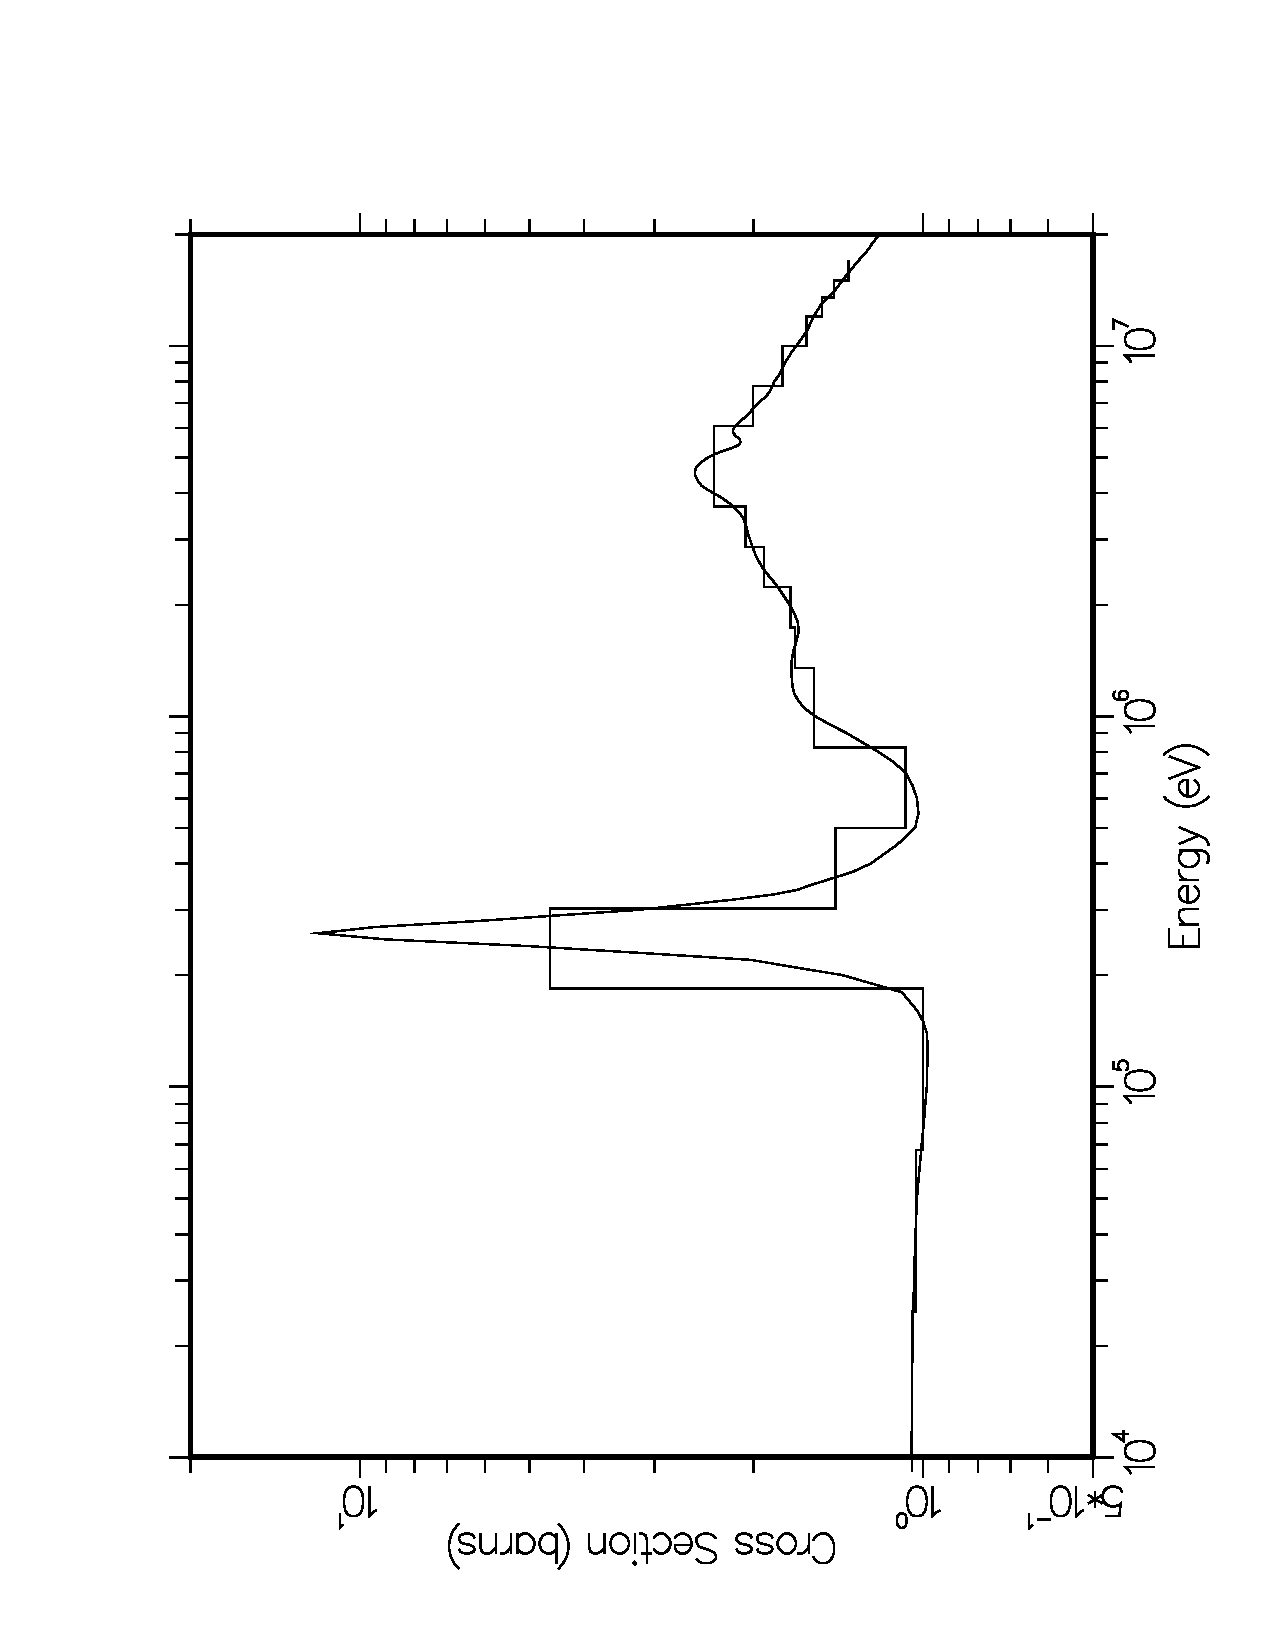
\includegraphics[keepaspectratio, height=3.5in, angle=270]{figs/groupr1ack}
\caption[Pointwise and multigroup cross section comparison]{A comparison
 of the pointwise and multigroup representations for the total cross section of
 $^{7}$Li.  The Los Alamos 30-group structure is shown.}
\label{gr1}
\end{figure}

\subsection{Weighting Flux}
\label{ssGROUPR_WtFlux}

In general, the weighting flux\index{weighting flux} $\phi$ is not
known; it is, after all, the particle distribution being sought
in the transport calculation.  However, it is often possible
to obtain fairly accurate group constants for a particular
application if the shape of the flux is reasonably well known
over the broad energy ranges of a particular few-group structure
(for example, a fission spectrum, thermal Maxwellian, or $1/E$
slowing-down spectrum). Alternatively, one can use many small groups
so that mistakes in guessing the shape inside the group are not very
important.  The key to using the multigroup method effectively is
balancing the tradeoffs between the choice of weight function and
the number of groups used for each different class of problem being solved.

In many cases of practical interest, the flux $\phi$ will contain dips
corresponding to the absorption resonances of the various materials.
In the reaction rate $\sigma(E)\times\phi(E)$, these dips clearly reduce
(self-shield) the effect of the corresponding resonance.  GROUPR provides
two methods to estimate the effect of this self-shielding: the Bondarenko
model and the flux calculator.
\index{self-shielding}
\index{Bondarenko method}
\index{flux calculator}

In the Bondarenko model\cite{Bondarenko}, the narrow resonance (NR)
approximation\index{narrow resonance approximation}, and the
B$_{\rm N}$ approximation for large systems\cite{ref5} are invoked
to obtain

  \begin{equation}
    \phi_{\ell}(E)={{W_{\ell}(E)}\over{[\sigma_t(E)]^{\ell+1}}}\,\,,
  \end{equation}

\noindent
where $\phi_{\ell}$ is the $\ell$-th Legendre component of the angular
flux, the $W_\ell(E)$ are smooth functions of energy (such as $1/E$+fission),
and $\sigma_t(E)$ is the total macroscopic cross section for the material.
GROUPR takes all of the $W_{\ell}$ to be equal to the single function $C(E)$,
where $C(E)$ can be read in or set to one of several internally defined
functions.  It is further assumed that the important self-shielding effect
of the flux can be obtained for isotope $i$ by representing all the other
isotopes with a constant ``background cross section'', $\sigma_0$.  Therefore,
\index{background cross section}
\index{$\sigma_0$}

   \begin{equation}
    \phi_{\ell}^i(E)={{C(E)}\over
    {[\sigma_t^i(E)+\sigma_0^i]^{\ell+1}}} \,\,,
  \label{Eq14}
  \end{equation}

\noindent
where $\sigma_t^i$ is the microscopic total cross section for isotope $i$.
The qualitative behavior of Eq.~\ref{Eq14} is easy to understand.
If $\sigma_0$ is larger than the tallest peaks in $\sigma_t$, the weighting
flux $\phi$ is approximately proportional to the smooth weighting function
$C(E)$.  This is called infinite dilution\index{infinite dilution};
 the cross section in the material of interest has little or no effect
on the flux.  On the other hand, if $\sigma_0$ is small with respect
to $\sigma_t$, the weighting flux will have large dips at the locations
of the peaks in $\sigma_t$, and a large self-shielding effect will
be expected.

Each component material of a mixture has a different weight function.
The macroscopic total cross sections are given by

  \begin{equation}
    \sigma_{t\ell g}=\sum_i \rho_i \,\sigma_{t\ell g}^i(\sigma_0^i,T)\,\,,
  \end{equation}

\noindent
where

  \begin{equation}
    \sigma_{t\ell g}^i(\sigma_0,T)=
    {{\displaystyle\int_g {{\sigma_t^i(E,T)}\over
    {[\sigma_0+\sigma_t^i]^{\ell+1}}}
    C(E)\,dE}\over
    {\displaystyle\int_g{{1}\over
    {[\sigma_0+\sigma_t^i]^{\ell+1}}} C(E)\,dE}}\,\,.
  \end{equation}

\noindent
Similar equations are used for $\sigma_R$ and $\sigma_{X\ell g\rightarrow g'}$.
On the GROUPR level, $\sigma_0$ and $T$ are simply parameters.  Subsequent
codes, such as 1DX\cite{1DX}\index{1DX} or TRANSX\cite{TRANSX,TRANSX2},
\index{TRANSX} can compute an appropriate value for $\sigma_0$, and then
interpolate in tables of cross section versus $\sigma_0$ and $T$ to get
the desired self-shielded group constants.

The appropriate value for $\sigma_0^i$\index{$\sigma_0$} is obvious
when a single resonance material is mixed with a moderator material
(for example, $^{238}$UO$_2$), because the admixed materials typically
have a constant cross section in the energy range where the heavy isotopes
have resonances.  For a mixture of resonance materials, the normal procedure
is to preserve the average of Eq.~\ref{Eq14} in each group by using

  \begin{equation}
    \sigma_{0g}^i={{1}\over{\rho_i}}
    \sum_{j\ne i}\rho_j \,\sigma_{t0g}^j(\sigma_{0g}^j,T)\,\,,
  \label{Eq17}
  \end{equation}

\noindent
where the $\rho_i$ are atomic densities or atomic fractions.
Eq.~\ref{Eq17} is solved by iteration.  Interference between resonances
in different materials is handled in an average sense only.

In the unresolved energy range\index{unresolved resonance range}
(see \hyperlink{sUNRESRhy}{UNRESR}\index{UNRESR} and
\hyperlink{sPURRhy}{PURR}\index{PURR}), the explicit dependence
of cross section on energy is not known.  The integrands are replaced
by their expected values

  \begin{equation}
    \sigma_{x\ell g}(\sigma_0)=
    {\displaystyle{\int_g\biggl<{{\sigma_x}\over{[\sigma_0+\sigma_t]^{\ell+1}}}
    \,\biggr>W_{\ell}\,dE}
    \over\displaystyle{\int_g\biggl<{1\over{[\sigma_0+\sigma_t]^{\ell+1}}}
    \,\biggr>W_{\ell}\,dE}}\,\,,
  \label{Eq18}
  \end{equation}

\noindent
where the expected values are averages over the distributions of
resonance position and width expected in the vicinity of energy $E$.
The \hyperlink{sUNRESRhy}{UNRESR} and \hyperlink{sPURRhy}{PURR}
modules produce effective self-shielded point
cross sections defined by

  \begin{equation}
    \bigl<\sigma_x\bigr>_{\ell}=
    {{\displaystyle{\biggl<{{\sigma_x}\over{[\sigma_0
    +\sigma_t]^{\ell+1}}}}\biggr>}
    \over\displaystyle{\biggl<
    {1\over{[\sigma_0+\sigma_t]^{\ell+1}}}\biggr>}}\,\,.
  \label{Eq19}
  \end{equation}

\noindent
Substituting Eq.~\ref{Eq19} into Eq.~\ref{Eq18} gives an equation of
the form of Eqs.~\ref{Eq10} and \ref{Eq11}, except that $\sigma$ is
replaced by $\bigl<\sigma\bigr>$, and the flux is replaced by an average
effective flux.  This effective flux can be obtained by manipulating the
effective total cross section as follows:

  \begin{equation}
    \bigl<\sigma_t\bigr>_{\ell}=
    {\displaystyle{\biggl<{{\sigma_0+\sigma_t-\sigma_0}
    \over{[\sigma_0+\sigma_t]^{\ell+1}}}\biggr>}
    \over\displaystyle{\biggl<{{1}\over
    {[\sigma_0+\sigma_t]^{\ell+1}}}\biggr>}}
    ={\displaystyle{\biggl<{1
    \over{[\sigma_0+\sigma_t]^{\ell}}}\biggr>}
    \over\displaystyle{\biggl<{{1}\over
    {[\sigma_0+\sigma_t]^{\ell+1}}}\biggr>}}-\sigma_0\,\,,
  \end{equation}

\noindent
from which

  \begin{equation}
    \biggl<{{1}\over{[\sigma_0+\sigma_t]^{\ell+1}}}\biggr>
    = {\displaystyle{\biggl<{{1}\over{[\sigma_0+\sigma_t]^{\ell}}}\biggr>}
    \over{\sigma_0+\bigl<\sigma_t\bigr>_k}}\,\,.
  \label{Eq21}
  \end{equation}

\noindent
Eq.~\ref{Eq21} defines a recursion relation which can be used to compute
the effective flux to any order

  \begin{equation}
    \biggl<{{1}\over{[\sigma_0+\sigma_t]^{\ell+1}}}\biggr>
    = \prod_{k=0}^{\ell}{1\over{\sigma_0+\bigl<\sigma_t\bigr>_k}}\,\,,
  \label{Eq22}
  \end{equation}
\vspace{0.5 pt}

\noindent
This equation reduces to Eq.~\ref{Eq14} in the resolved range.  It is
the formula used in \cword{genflx} to compute $\phi_{\ell}(E)$ for the
Bondarenko option.

When heterogeneity\index{heterogeneity} effects are important, the
background cross section method can be extended as follows.  In an
infinite system of two regions (fuel and moderator), the neutron
balance equations are

  \begin{equation}
    V_f\sigma_f\phi_f=(1-P_f)V_f S_f+P_m V_m S_m\,\,,
  \end{equation}

\noindent
and

  \begin{equation}
    V_m\sigma_m\phi_m=P_f V_f S_f+(1-P_m)V_m S_m\,\,,
  \end{equation}

\noindent
where $V_f$ and $V_m$ are the region volumes, $\sigma_f$ and $\sigma_m$
are the corresponding total macroscopic cross sections, $S_f$ and $S_m$
are the sources per unit volume in each region, $P_f$ is the probability
that a neutron born in the fuel will suffer its next collision in the
moderator, and $P_m$ is the probability that a neutron born in the
moderator will suffer its next collision in the fuel.  As usual, use
is made of the reciprocity theorem,
\index{reciprocity theorem}

  \begin{equation}
    V_f\sigma_f P_f=V_m\sigma_m P_m \,\,,
  \end{equation}

\noindent
and the Wigner rational approximation\index{Wigner rational approximation}
to the fuel escape probability,

  \begin{equation}
    P_f={{\sigma_e}\over{\sigma_e+\sigma_f}}\,\,,
  \end{equation}

\noindent
where $\sigma_e$ is a slowly varying function of energy called the escape
cross section\index{escape cross section}, to obtain an equation for the
fuel flux in the form

  \begin{equation}
    (\sigma_f+\sigma_e)\phi_f={{\sigma_e S_m}\over \sigma_m} +S_f \,\,.
  \label{Eq27}
  \end{equation}

\noindent
In the limit where the resonances are narrow with respect to both fuel
and moderator scattering, the source terms $S_f$ and $S_m$ take on their
asymptotic forms of $\sigma_p/E$ and $\sigma_m/E$ respectively, and this
equation becomes equivalent to the Bondarenko model quoted above with

  \begin{equation}
    \sigma_0^f={\sigma_e \over \rho_f}\,\,,
  \label{Eq28}
  \end{equation}

\noindent
and

  \begin{equation}
    C(E)={{\sigma_e+\sigma_p}\over{\rho_f E}}\,\,.
  \end{equation}

\noindent
Note that a large escape cross section (a sample that is small relative
to the average distance to collision), corresponds to infinite dilution
as discussed above.  To illustrate the general case, consider a neutron
traveling through a lump of uranium oxide with an energy close to a
resonance energy.  If the neutron scatters from an oxygen nucleus, it
will lose enough energy so that it can no longer react with the uranium
resonance.  Similarly, if the neutron escapes from the lump, it can no
longer react with the uranium resonance.  The processes of moderator
scattering and escape are equivalent in some way.  Comparing
Eq.~\ref{Eq28} with Eq.~\ref{Eq17} gives an
\index{equivalence principle} ``equivalence principle''
that says that a lump of particular dimensions and a mixture of
particular composition will have the same self-shielded cross sections
when the narrow resonance approximation is valid.  The effects of
material mixing and escape can simply be added to obtain the effective
$\sigma_0$ for a lump containing admixed moderator material.  Therefore,
Eq.~\ref{Eq17} is extended to read

  \begin{equation}
    \sigma_{0g}^i ={{1} \over {\rho_i}}
    \biggl\lbrace \sigma_e +
    \sum_{j\ne i} \rho_j \,\sigma_{t0g}^j
    (\sigma_{0g}^j ,T) \biggr\rbrace \,\,,
  \end{equation}

\noindent
where the escape cross section for simple convex objects (such as plates,
spheres, or cylinders) is given by $(4V{/}S)^{-1}$, where $V$ and $S$
are the volume and surface area of the object, respectively.  Many codes
that use the background cross section method modify the escape cross section
as defined above to correct for errors in the Wigner rational
approximation (``Bell factor''\index{Bell factors},
``Levine factor'' \index{Levine factors}), or to correct for
the interaction between different lumps in the moderating region
(``Dancoff corrections'')\index{Dancoff corrections}.  These
enhancements will not be discussed here.

As an example of self-shielded cross sections and how they vary
with the background cross section, Fig.~\ref{u238ng} shows the
first three capture resonances of $^{238}$U (which are very important
for thermal power reactors) at room temperature for $\sigma_0$
values ranging from infinity down to 10 barns.  Background cross
sections that range between 20 and 50 barns are typical for
uranium-oxide pin cells.

\begin{figure}[tp]\centering
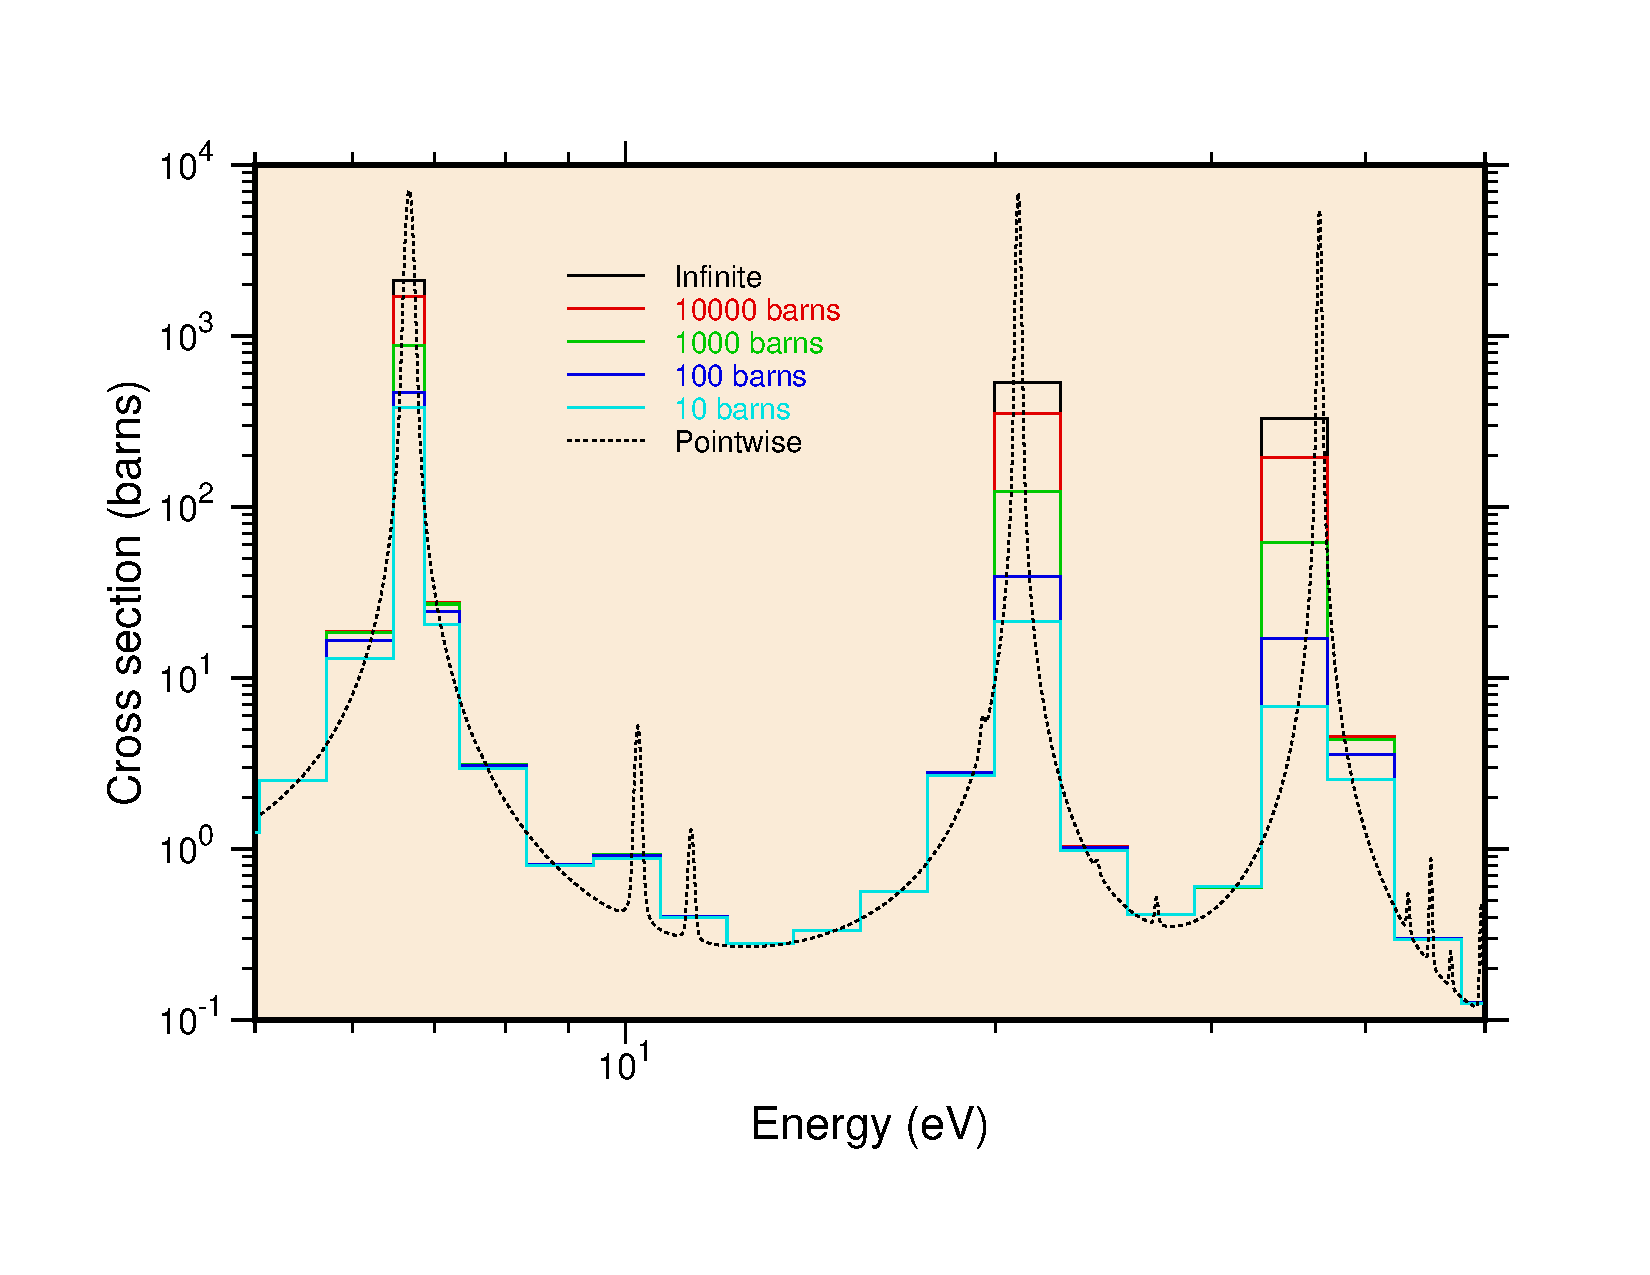
\includegraphics[keepaspectratio, height=3.2in, angle=0]{figs/u238ngack}
\caption[The self-shielding effect on the first three $^{238}$U capture
 resonances.]{The self-shielding effect on the first three $^{238}$U
 capture resonances at room temperature in the 5 to 50 eV range.  The
 multigroup boundaries are from the Los Alamos 187-group structure.}
\label{u238ng}
\end{figure}

\begin{figure}[bp]\centering
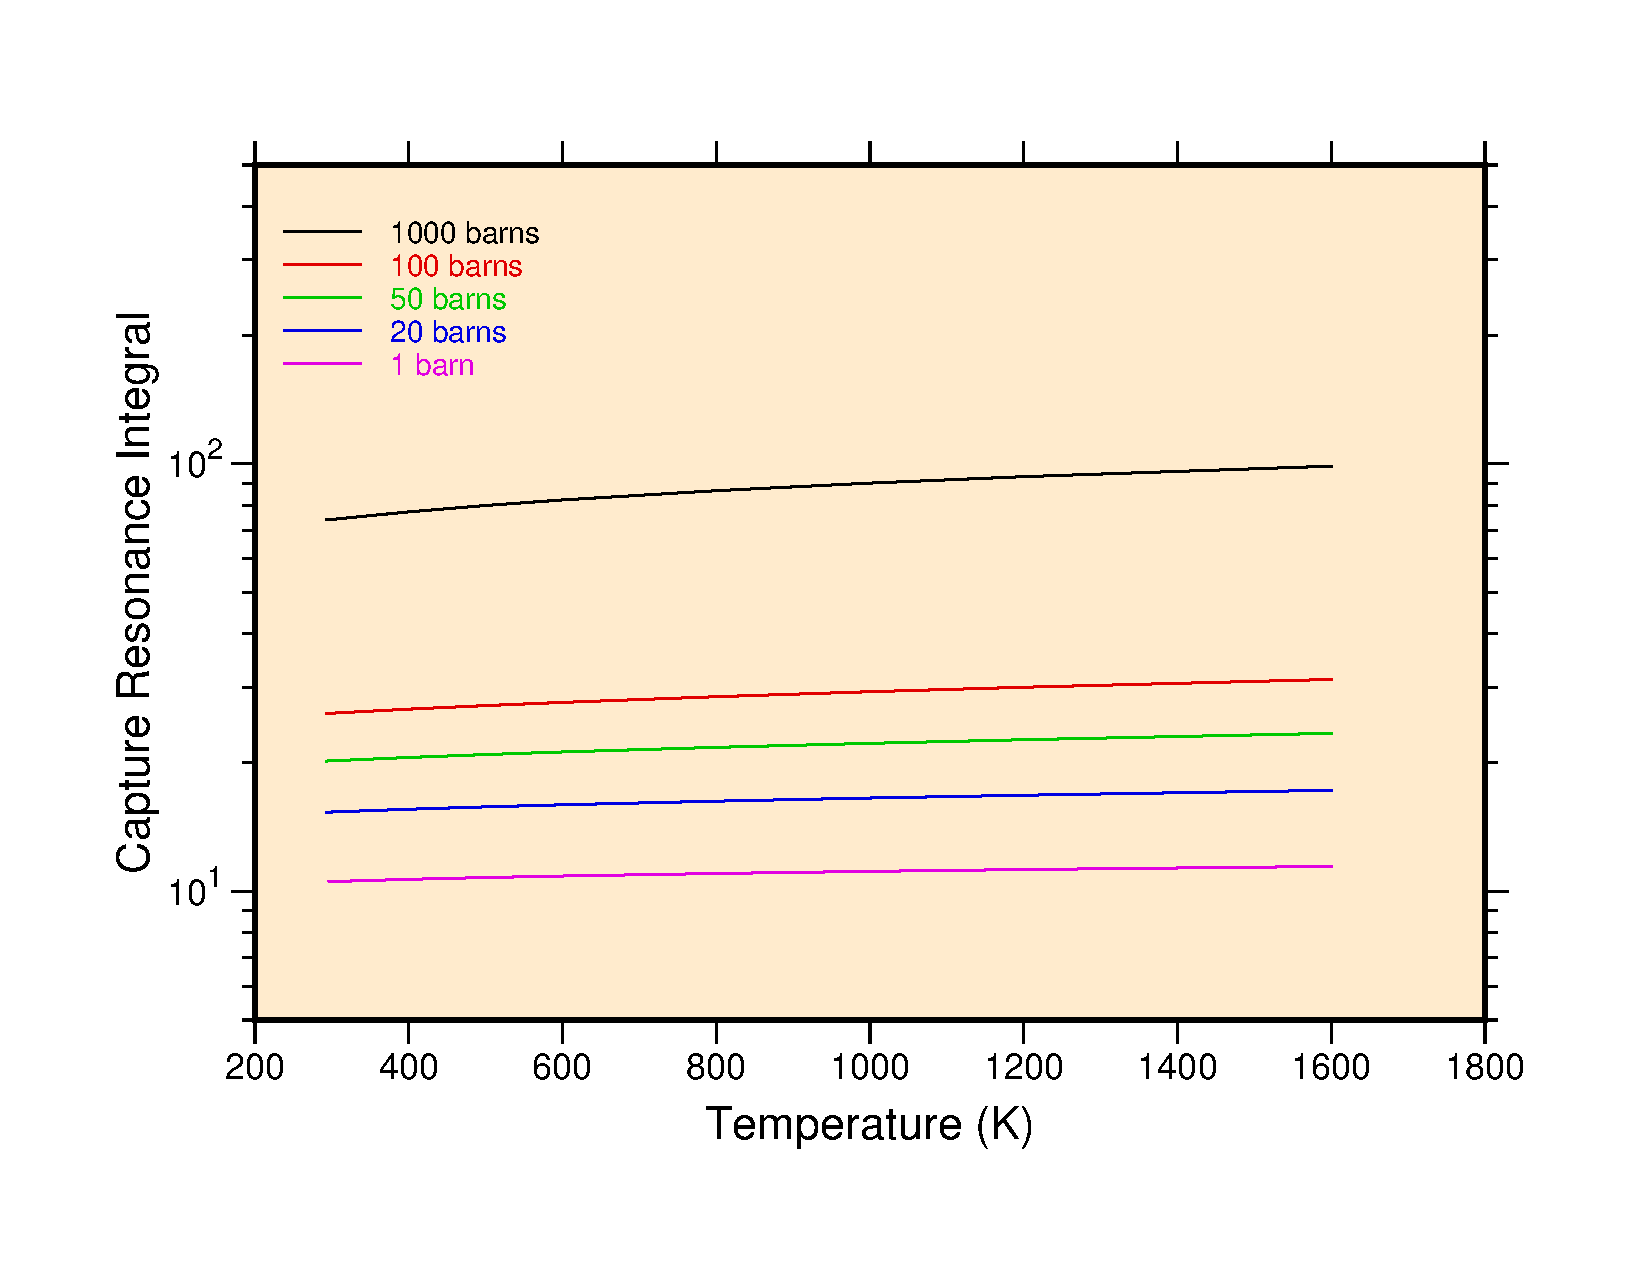
\includegraphics[keepaspectratio, height=3.2in, angle=0]{figs/u238riack}
\caption[$^{238}$U capture resonance integral versus temperature and
 background cross section]{The capture resonance integral for $^{238}$U
 showing its variation with temperature and background cross section
 $\sigma_0$.  The resonance integral at infinite dilution is 275.58 barns.  Note
 the slope with temperature, which helps to produce a negative temperature
 coefficient for uranium systems.}
\label{u238ri}
\end{figure}

The \hyperlink{sBROADRhy}{BROADR} chapter of this report
showed its capability to
compute standard resonance integrals.  However, when self shielding
and material temperature come into play, the effective resonance
integral changes.  GROUPR can calculate these quantities by doing
one-group calculations with $1/E$ weighting over a standard energy
range. Using the range 0.5 eV to the upper limit of the evaluation
will match what \hyperlink{sBROADRhy}{BROADR} does.  Fig.~\ref{u238ri}
shows the temperature
dependence of the capture resonance integral for $^{238}$U from
ENDF/B-VII at several different background cross sections.  The range between
20 and 50 barns is typical for reactor pin cells.


\subsection{Flux Calculator}
\label{ssGROUPR_FluxCalc}

This narrow-resonance approach is quite useful for practical fast
reactor problems.  However, for nuclear systems sensitive to energies
from 1 to 500 eV, there are many broad- and intermediate-width resonances
which cannot be self-shielded with sufficient accuracy using the
Bondarenko approach.  The GROUPR flux calculator\index{flux calculator}
is designed for just such problems.

Consider an infinite homogeneous mixture of two materials and assume
isotropic scattering in the center-of-mass system.  The integral
slowing-down equation becomes

  \begin{eqnarray}
    \sigma(E)\,\phi(E)&=&\int_E^{E/\alpha_1}{{\sigma_{s1}(E')}\over
    {(1-\alpha_1)E'}}\,\phi(E')\,dE'\nonumber\\
    &+&\int_E^{E/\alpha_2}{{\sigma_{s2}(E')}\over
    {(1-\alpha_2)E'}}\,\phi(E')\,dE'\,\,.
  \end{eqnarray}

\noindent
Furthermore, assume that material 1 is a pure scatterer with constant
cross section and transform to the $\sigma_0$ representation.  The
integral equation becomes

  \begin{eqnarray}
    [\sigma_0+\sigma_{t2}(E)]\,\phi(E)&=&
    \int_E^{E/\alpha_1}{{\sigma_0}\over
    {(1-\alpha_1)E'}}\,\phi(E')\,dE'\nonumber\\
    &+&\int_E^{E/\alpha_2}{{\sigma_{s2}(E')}\over
    {(1-\alpha_2)E'}}\,\phi(E')\,dE'\,\,.
  \end{eqnarray}

\noindent
Finally, assume that the moderator (material 1) is light enough so that
all the resonances of material 2 are narrow with respect to scattering
from material 1.  This allows the first integral to be approximated by
its asymptotic form, $1/E$.  More generally, the integral is assumed to
be a smooth function of $E$ given by $C(E)$.  In this way, material 1
can represent a mixture of other materials just as in the Bondarenko
method.  Fission source and thermal upscatter effects can also be lumped
in $C(E)$.  The integral equation has now been reduced to

  \begin{equation}
    [\sigma_0+\sigma_t(E)]\,\phi(E)={C(E)\,\sigma_0}
    +\int_E^{E/\alpha}{{\sigma_s(E')}\over
    {(1-\alpha)E'}}\,\phi(E')\,dE'\,\,.
  \label{Eq33}
  \end{equation}

\noindent
This is the simplest problem that can be solved using the flux calculator.
The results still depend on the single parameter $\sigma_0$, and they
can be used easily by codes that accept Bondarenko cross sections.

For heterogeneous problems, when the narrow-resonance approximation
fails, both $S_f$ and $S_m$ in Eq.~\ref{Eq27} will show resonance features.
To proceed further with the solution of this equation, it is necessary
to eliminate the moderator flux that is implicit in $S_m$.  As
a sample case, consider a fuel pin immersed in a large region of
water.  The fission neutrons appear at high energies, escape from the
pin, slow down in the moderator (giving a $1/E$ flux), and are absorbed
by the resonances in the pin.  In this limit, any dips in the moderator
flux caused by resonances in the fuel are small.  On the other hand, in
a closely packed lattice, the flux in the moderator is very similar to
the flux in the fuel, and resonance dips in the moderator flux become
very evident.  Intermediate cases can be approximated\cite{ref9} by assuming

  \begin{equation}
    \phi_m=(1-\beta)\,{C(E)}+\beta\phi_f\,\,,
  \end{equation}

\noindent
where $\beta$ is a heterogeneity parameter given by

  \begin{equation}
    \beta={{V_f\sigma_e}\over{V_m\sigma_m}}\,\,.
  \end{equation}

\noindent
Note that $\beta\rightarrow 0$ gives the isolated rod limit and
$\beta\rightarrow 1$ gives the close-packed lattice limit.  This
substitution reduces the calculation of the fuel flux to

  \begin{equation}
    (\sigma_f+\sigma_e)\,\phi_f=(1-\beta)\,
    {C(E)\,\sigma_e }+S_\beta\,\,,
  \end{equation}

\noindent
where $S_\beta$ is the source term corresponding to a homogeneous mixture
of the fuel isotopes with the isotopes from the moderator region changed
by the factor $\beta\sigma_e/\sigma_m$.  If the fuel and moderator each
consisted of a single isotope and for isotropic scattering in the
center-of-mass system, the integral equation would become

  \begin{eqnarray}
    [\sigma_0+\sigma_t(E)]\,\phi_f(E)&=&
    (1-\beta)\,{C(E)\,\sigma_0}\nonumber\\
    &+&\int_E^{E/\alpha_m}{{\beta\sigma_0}\over
    {(1-\alpha_m)E'}}\,\phi_f(E')\,dE'\nonumber\\
    &+&\int_E^{E/\alpha_f}{{\sigma_{sf}(E')} \over
    {(1-\alpha_f)E'}}\,\phi_f(E')\,dE'\,\,,
  \label{Eq37}
  \end{eqnarray}

\noindent
where $\sigma_0$ is $\sigma_e$ divided by the fuel density (units are
barns/atom), $\alpha_m$ and $\alpha_f$ are the maximum fractional
energy change in scattering for the two isotopes, and $\sigma_{sf}(E')$
is the fuel scattering cross section.

This result has a form parallel to that of Eq.~\ref{Eq33}, but the
solution depends on the two parameters $\beta$ and $\sigma_0$.  For any
given data set, $\beta$ must be chosen in advance.  This might not be
difficult if the data are to be used for one particular system, such as
pressurized water reactors.  The routine also has the capability to
include one more moderator integral with a different $\alpha$ value and
a constant cross section.  The full equation is

  \begin{eqnarray}
    [\sigma_0+\sigma_t(E)]\,\phi_f(E)&=&
    (1-\beta)\,{C(E)\,\sigma_0}\nonumber\\
    &+&\int_E^{E/\alpha_3}{{\beta(1-\gamma)(\sigma_0-\sigma_{am}}\over
    {(1-\alpha_3)E'}}\,\phi_f(E')\,dE'\nonumber\\
    &+&\int_E^{E/\alpha_2}{{\sigma_{am}+\beta\gamma(\sigma_0-\sigma_{am}}\over
    {(1-\alpha_2)E'}}\,\phi_f(E')\,dE'\nonumber\\
    &+&\int_E^{E/\alpha_f}{{\sigma_{sf}(E')} \over
    {(1-\alpha_f)E'}}\,\phi_f(E')\,dE'\,\,,
  \label{Eq37a}
  \end{eqnarray}

\noindent
where $\sigma_{am}$ is the cross section of the admixed moderator
(with energy loss $\alpha_2$), and $\gamma$ is the fraction of the
admixed moderator that is mixed with the external moderator (which has
energy loss $\alpha_3$).  This allows calculations with H$_2$O as the
moderator and an oxide as the fuel.  The flux calculator can thus obtain
quite realistic flux shapes for a variety of fuel, admixed moderator and
external moderator combinations.  An example comparing the Bondarenko
flux with a more realistic computed flux is given in Fig.~\ref{gr2}.

\begin{figure}[thb]\centering
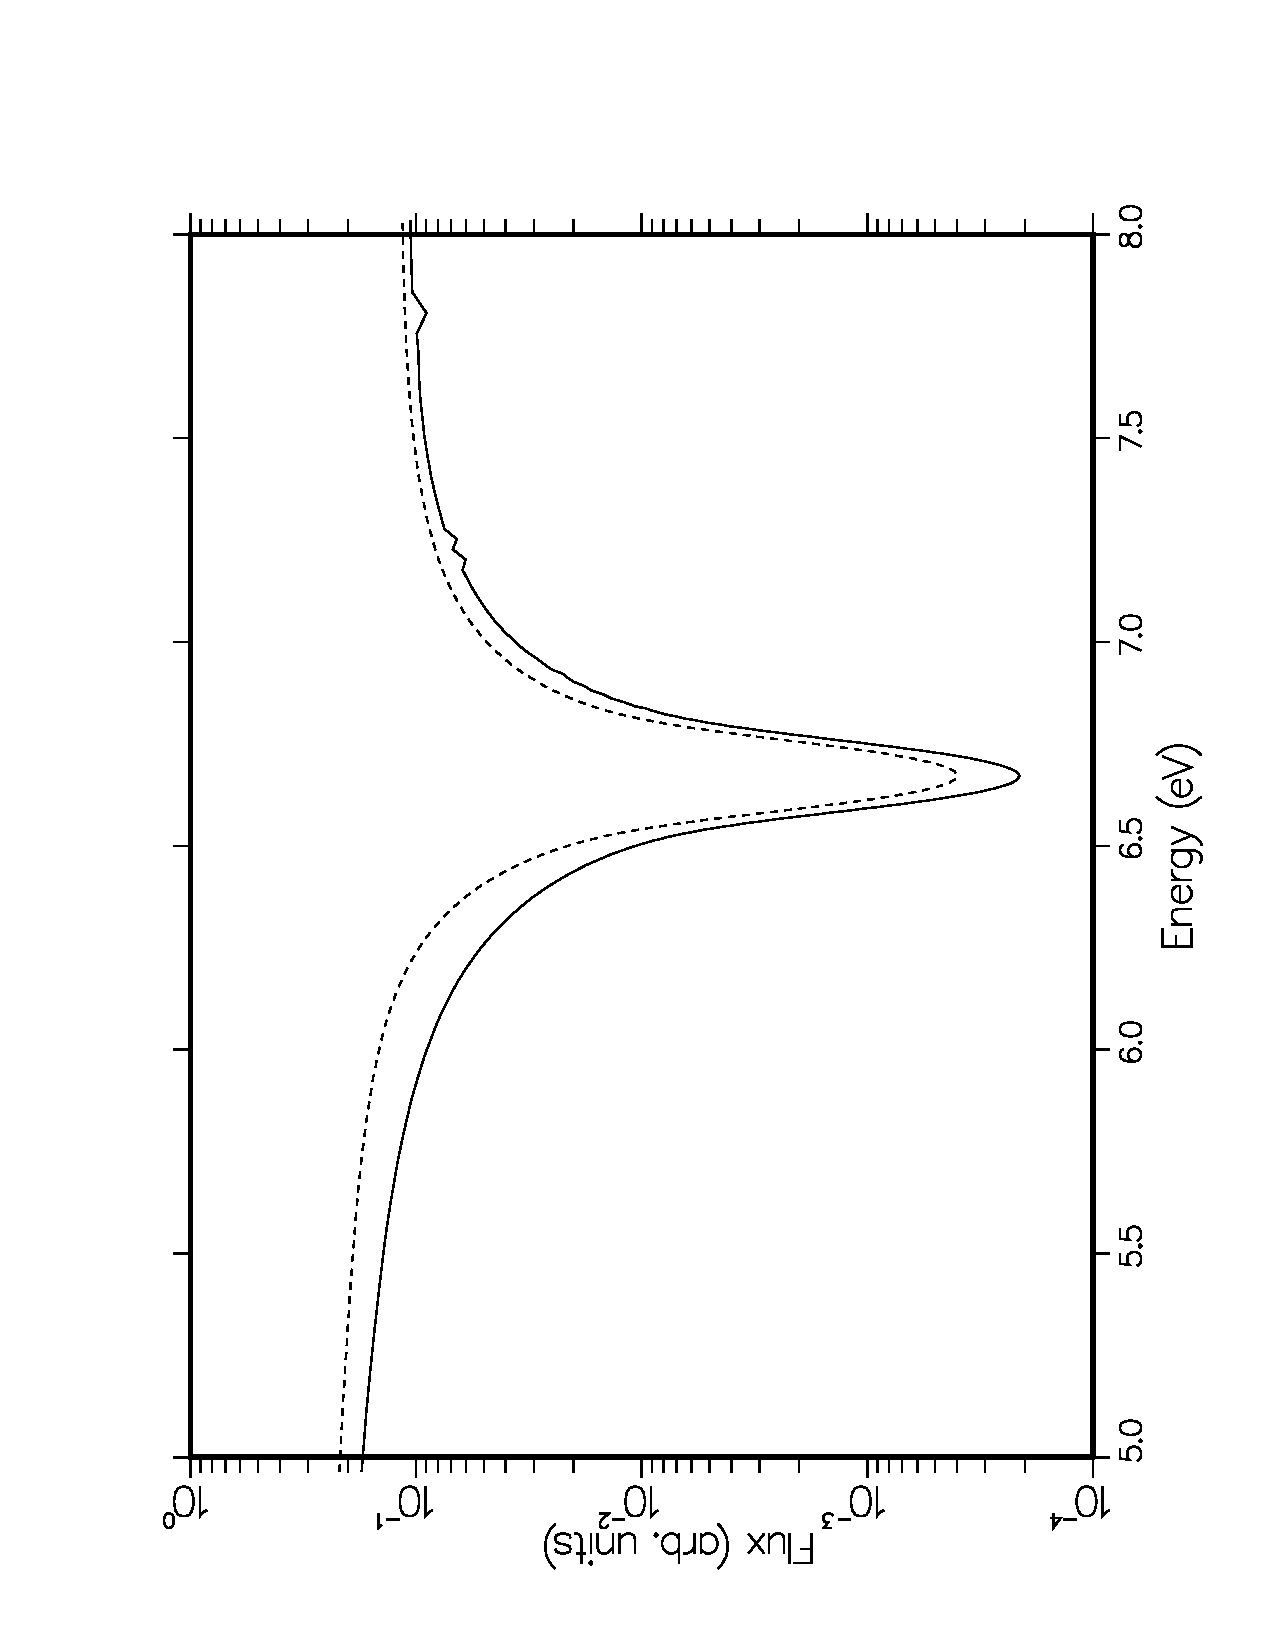
\includegraphics[keepaspectratio, height=3.5in, angle=270]{figs/groupr2ack}
\caption[Flux model predictions for $^{238}$UO$_2$ in water in the region
 near the 6.7 eV $^{238}$U resonance]{A comparison of the Bondarenko flux
 model (dashed) with a realistic computed flux (solid) for a $^{238}$U oxide
 pin in water in the region of the 6.7 eV resonance.}
\label{gr2}
\end{figure}

In practice, a fuel rod rarely contains only one resonance isotope.
\index{resonance interference}
As an example, consider a mixture of a few percent of $^{239}$Pu
with $^{238}$U as the major component.  There will be a strong dip in the
flux associated with the 6.7 eV $^{238}$U resonance that will affect the
flux in the region of the 7.8 eV $^{239}$Pu resonance (the interference
effect), and there will also be a dip in the flux corresponding to the
7.8 eV resonance (the self-shielding effect).  This additional
complication in the flux shape would be expected to change the group
constants for $^{239}$Pu since both features lie in the same group for
typical group structures.  However, the effect of the $^{239}$Pu on the
$^{238}$U group constants should be minimal.  This argument suggests that
the full flux calculation be used for $^{238}$U as a single resonance
material.  The resulting flux would then be used to estimate the flux
to be used in averaging the $^{239}$Pu cross sections as follows:

  \begin{equation}
    \phi_{239}(E,\sigma_0)={\displaystyle{\phi_{238}(E,50)}\over
    \displaystyle \sigma_0+{\displaystyle{\sigma_{239}(E)}\over\displaystyle
    {1+{\displaystyle{\sigma_{238}(E)\over\displaystyle 50}}}}}\,\,,
  \label{Eq38}
  \end{equation}
\vspace{0.5 pt}

\noindent
where the $^{238}$U flux is characteristic of a background of 50
barns/atom, which is representative of many thermal reactor systems.
This formula assumes that the effect of $^{239}$Pu on the scattering source
for the mixture is small, but it retains the absorption effects.  The
self-shielding of $^{239}$Pu is treated in the narrow resonance
approximation only.  The GROUPR flux calculator includes an option to
write out a file containing the calculated flux and cross section
needed for this formula ({\it e.g.}, for $^{238}$U) and another option
to skip the flux calculation and use the formula above to obtain the
weighting flux ({\it e.g.}, for $^{239}$Pu).

The slowing-down integral equation of Eq.~\ref{Eq33} or \ref{Eq37}
is solved point by point (see subroutine \cword{genflx}) using the
total and elastic cross sections on the PENDF tape produced by
\hyperlink{sRECONRhy}{RECONR}.
In order to keep this task within bounds, the flux is computed from the
lower limit of the first group to a specified energy \cword{fehi} or
until \cword{nfmax} values have been computed.  The flux at higher
energies is continued using the Bondarenko model described above.
\index{Bondarenko method}

\subsection{Fission Source}
\label{ssGROUPR_FissSource}

The fission source\index{fission source} was included in the
transfer cross section $\sigma_X$ in the development above.  It is
usually convenient to separate fission from scattering.  Assuming
isotropy, the source of fission neutrons into group $g$ is given by

  \begin{equation}
    S_g=\sum_{g'}\sigma_{fg'\rightarrow g}\,\phi_{0g'}\,\,,
  \end{equation}

\noindent
where the group-to-group matrix\index{fission matrix}
for fission is defined as in Eq.~\ref{Eq12}, but with $\ell$ equal
to zero.  Most existing transport codes do not use this matrix
form directly because the upscatter is expensive to handle and
a reasonably accurate alternative exists.  Except for relatively
high neutron energies, the spectrum of fission neutrons is only
weakly dependent on initial energy.  Therefore, the fission source
can be written

  \begin{equation}
    S_g=\chi_g\sum_{g'}\,\overline\nu_{g'}\,\sigma_{fg'}\,\phi_{0g'}\,\,,
  \end{equation}

\noindent
where $\overline\nu_g$ is the fission neutron yield, $\sigma_{fg}$ is the
fission cross section, and $\chi_g$ is the average fission spectrum
(the familiar ``chi'' vector\index{fission chi}), which can be defined by

  \begin{equation}
    \chi_g={\displaystyle{\sum_{g'}\sigma_{fg'\rightarrow g}\,\phi_{0g'}}
    \over\displaystyle{\sum_{g}\sum_{g'}\sigma_{fg'\rightarrow g}
    \,\phi_{0g'}}}\,\,.
  \label{Eq41}
  \end{equation}

\noindent
The fission neutron yield is given by
\index{fission neutron yield}

  \begin{equation}
    \overline\nu_{g}
    = \sum_{g'}\sigma_{fg\rightarrow g'}\,/\,\sigma_{fg}\,\,.
  \end{equation}

\noindent
Clearly, $\chi_g$ as given by Eq.~\ref{Eq41} depends on the flux in the
system of interest.  The dependence is weak except for high incident
energies, and a rough guess for $\phi_{0g}$ usually gives an accurate
spectrum.  When this is not the case, the problem can be iterated, or
the full matrix representation can be used.

It is possible to take advantage of the weak energy dependence of the
shape of the fission spectrum at low energies to reduce the time required
to process fission data, and to reduce the size of the fission data on the
output file.  GROUPR determines a break energy from File 5 such that
the fission spectrum is constant below this energy.  It only has to make
a single calculation of this spectrum $\chi^{LE}_g$.  Then it computes
a fission neutron production cross section $\sigma^{HE}_{fPg}$ for
groups below the break energy using the normal cross section processing
methods.  A full matrix $\sigma^{HE}_{fg'{\rightarrow}g}$ is computed
for groups above the break point.  As an example, consider using the
GROUPR 187-group structure and finding that there are 130 constant groups.
The 187${\times}$187 matrix is reduced to a 57${\times}$187 matrix,
a 187-element spectrum vector, and a 130-group production vector, for
a total reduction in size of 68\%.  The effective fission matrix is
given by

\begin{equation}
   \sigma_{fg'{\rightarrow}g}=\sigma^{HE}_{fg'{\rightarrow}g}
      + \chi^{LE}_g\sigma^{LE}_{fPg'} \,\,.
\end{equation}
\vspace{0.5 pt}

The fission matrix computed by GROUPR represents the prompt part
of fission only\index{prompt fission}.  The delayed component of
fission is represented\index{delayed fission} by a delayed-neutron
yield $\overline\nu_{g}^D$, decay constants for six (or sometimes 8)
time groups, $\lambda_i^D$, and emission probability spectra for
six (or 8) time groups, $\chi_{ig}^D$.  Steady-state fission
\index{fission, steady-state} can be obtained using

  \begin{equation}
    \overline\nu_g^{SS}=\overline\nu_g
    +\overline\nu_g^D\,\,,
  \end{equation}

\noindent
and

  \begin{equation}
    \chi_g^{SS}={\displaystyle{\sum_{g'}\sigma_{fg'\rightarrow g}\,\phi_{0g'}
    +\chi_g^D\sum_{g'}\overline\nu_{g'}^D\,\sigma_{fg'}\,\phi_{0g'}}
    \over\displaystyle{\sum_g\sum_{g'}\sigma_{fg'\rightarrow g}\,\phi_{0g'}
    +\sum_{g'}\overline\nu_{g'}^D\,\sigma_{fg'}\,\phi_{0g'}}}\,\,,
  \end{equation}

\noindent
where

  \begin{equation}
    \chi_g^D=\sum_i\chi_{ig}^D\,\,.
  \end{equation}

\noindent
Note that $\chi_g^D$ sums to unity, but the $\chi$ for each time group
sums to the fraction of the delayed neutron yield that appears
in that time group.
\index{delayed chi}
\index{delayed-neutron yield}

In ENDF-format files, the total fission reaction is represented
by MT=18.  Important isotopes also give the partial fission reactions
\index{partial fission} (n,f), (n,n$'$f), (n,2nf), and sometimes (n,3nf)
using MT=19, 20, 21, and 38 respectively.  The MT=18 representation is
adequate for most fission reactor applications, but the partial reactions
should be processed for applications with significant flux above 6 MeV.
Caution:  although the cross section for MT=18 equals the sum of its
parts, the group-to-group fission matrix $\sigma_{fg\rightarrow g'}$
computed from MT=18 will not, in general, equal the sum of the
partial matrices for MT=19, 20, 21, and 38 above the 6-MeV threshold
for second-chance fission.  The breakup into partial fission matrices
has not been used in recent ENDF/B-VII evaluations.  The
delayed neutron data are given in MT=455.  Sample input instructions
for processing the various combinations of fission reactions used
in ENDF/B will be found in Section~\ref{ssGROUPR_Continuum}.  GROUPR outputs all
the components of fission separately in order to give succeeding
modules or codes complete flexibility.

\subsection{Diffusion Cross Sections}
\label{ssGROUPR_Diffusion}

The diffusion equation is often used in reactor physics
calculations.\index{diffusion constant}  Starting with
Eq.~\ref{Eq7}, use the Legendre expansion
for $\phi_g$ in the derivative term, and make use of the recursion
relation for $\mu P_{\ell}(\mu)$ and the orthogonality relation for
the Legendre polynomials to obtain the transport equation in
spherical-harmonic form

  \begin{eqnarray}
    {{n+1}\over{2n+1}}{{\partial\phi_{n+1,g}}\over{\partial x}}
    &+&{{n}\over{2n+1}}{{\partial\phi_{n-1,g}}\over{\partial x}}
    \,\sigma_{tng}\,\phi_{ng}\nonumber\\
    \mbox{ }\nonumber\\
    &=& \sum_{g'}\sigma_{sng'\rightarrow g}\,\phi_{ng'}+S_{fg}+Q_{ng}\,\,,
  \end{eqnarray}

\noindent
where the transfer term has been separated into a scattering term with
cross section $\sigma_s$, and a fission source term $S_f$.  When this set
of equations is truncated at $n={\rm N} $, the results are usually called
the ``P$_{\rm N}$ equations''.  For now, all terms with $n>1$ are dropped,
and $Q$ is assumed to be isotropic.  Thus,

  \begin{equation}
    {{\partial\phi_{1g}}\over{\partial x}}
    +\sigma_{t0g}\,\phi_{0g}
    =\sum_{g'}\sigma_{s0g'\rightarrow g}\,\phi_{0g'}
    +S_{fg}+Q_{0g}\,\,,
  \label{Eq47}
  \end{equation}

\noindent
and

  \begin{equation}
    {1\over 3}{{\partial\phi_{0g}}\over{\partial x}}
    +\sigma_{t1g}\,\phi_{1g}
    =\sum_{g'}\sigma_{s1g'\rightarrow g}\,\phi_{1g'}\,\,.
  \end{equation}

\noindent
The second equation can be written in the form of Fick's Law as follows:

  \begin{equation}
    \phi_{1g}=-D_g{{\partial\phi_{0g}}\over{\partial x}}\,\,,
  \end{equation}

  \begin{equation}
    D_g={1\over 3}\,{1\over\displaystyle{
    \sigma_{t1g}-{\displaystyle{\sum_{g'}\sigma_{s1g'\rightarrow g}
    \,\phi_{1g'}}\, / \,\displaystyle{\phi_{1g}}}}}\,\,,
  \label{Eq50}
  \end{equation}

\noindent
where $D_g$ is the diffusion constant.  The term in the denominator of
the second factor is the transport cross section for diffusion,
$\sigma_{trD}$.  Unfortunately, it depends on a fairly complete knowledge
of the neutron current in the system, perhaps from a previous calculation.
However, for many problems, $\sigma_{trD}$ can be simplified by assuming that

  \begin{equation}
    \sum_{g'}\sigma_{s1g'\rightarrow g}\,\phi_{1g'}\approx
    \sum_{g'}\sigma_{s1g\rightarrow g'}\,\phi_{1g}\,\,,
  \end{equation}

\noindent
with the result that

  \begin{equation}
    \sigma_{trD,g}=\sigma_{t1g}-\sum_{g'}\sigma_{s1g\rightarrow g'}\,\,,
  \label{Eq52}
  \end{equation}

\noindent
or

  \begin{equation}
    \sigma_{trD,g}=\sigma_{t1g}-\overline\mu_g\,\sigma_{s0g}\,\,,
  \end{equation}

\noindent
where $\overline\mu_g$ is the average scattering cosine for neutrons
in group $g$.  These forms depend only on the shape of the weighting
flux within the group, as usual.  Substituting for $\phi_{1g}$ in
Eq.~\ref{Eq47} gives

  \begin{equation}
    {{\partial}\over{\partial x}}\bigl(-D_g
    {{\partial\phi_{0g}}\over{\partial x}}\bigr)
    +\sigma_{0tg}\,\phi_{0g}
    =\sum_{g'}\sigma_{s0g'\rightarrow g}\,\phi_{0g'}
    +S_{fg}+Q_{0g}\,\,,
  \end{equation}

\noindent
which is the standard diffusion equation in slab geometry.  Neither the
diffusion coefficient nor the transport cross section for diffusion is
produced directly by GROUPR.  However, the components such a
$\sigma_{t\ell}$ and $\sigma_{s0g'\rightarrow g}$ are made available
to subsequent modules.

\subsection{Cross Sections for Transport Theory}
\label{ssGROUPR_Transport}

The S$_{\rm N}$ (discrete ordinates) transport codes solve the equation
\index{discrete-ordinates transport}
\index{S$_{\rm N}$ transport}

  \begin{eqnarray}
    \mu{{\partial}\over{\partial x}}\phi_g(\mu,x)
    &+&\sigma_g^{SN}\phi_g(\mu,x)\nonumber\\
    &=&\sum_{\ell=0}^N{{2\ell+1}\over{2}}P_{\ell}(\mu)
    \sum_{g'}\sigma_{s\ell g'\rightarrow g}^{SN}(x)\,\phi_{\ell g'}
    \nonumber\\
    &+&S_{fg}+Q_g(\mu,x)\,\,,
  \label{Eq55}
  \end{eqnarray}

\noindent
where once again one-dimensional slab geometry has been used for
simplicity.\footnote{The following development is based on the work of
Bell, Hansen, and Sandmeier\cite{ref10}.} By comparing Eq.~\ref{Eq55}
with Eq.~\ref{Eq7}, it is seen that the S$_{\rm N}$ equations require
the following cross sections:

  \begin{equation}
    \sigma_{s\ell g'\rightarrow g}^{SN}=\sigma_{s\ell g'\rightarrow g}
    ,\qquad g'\ne g\,\,,
  \end{equation}

\noindent
and

  \begin{equation}
    \sigma_{s\ell g\rightarrow g}^{SN}=\sigma_{s\ell g\rightarrow g}
    -\sigma_{t\ell g}+\sigma_g^{SN}\,\,,
  \end{equation}

\noindent
where $\sigma_g^{SN}$ is not determined and can be chosen to improve
the convergence of the S$_N$ calculation.  A particular choice of
$\sigma_g^{SN}$ gives rise to a ``transport approximation'',
\index{transport approximations}
and various recipes are in use, such as:

Consistent-P approximation:

  \begin{equation}
    \sigma_g^{SN}=\sigma_{t0g}\,\,.
  \end{equation}

Inconsistent-P approximation:

  \begin{equation}
    \sigma_g^{SN}=\sigma_{t,N+1,g}\,\,.
  \end{equation}

Diagonal transport approximation:

  \begin{equation}
    \sigma_g^{SN}=\sigma_{t,N+1,g}-\sigma_{s,N+1,g\rightarrow g}\,\,.
  \end{equation}

Bell-Hansen-Sandmeier (BHS) or extended transport approximation:

  \begin{equation}
    \sigma_g^{SN}=\sigma_{t,N+1,g}-\sum_{g'}\sigma_{s,N+1,g\rightarrow g'}\,\,.
  \end{equation}

Inflow transport approximation:

  \begin{equation}
    \sigma_g^{SN}=\sigma_{t,N+1,g}-{\displaystyle
    {\sum_{g'}\sigma_{s,N+1,g'\rightarrow g}\,\phi_{N+1,g'}}
    \over\displaystyle{\phi_{N+1,g}}}\,\,.
  \end{equation}

\noindent
The first two approximations are most appropriate when the scattering orders
above N are small.  The inconsistent option removes most of the delta
function of forward scattering introduced by the correction for the
anisotropy of the total scattering rate, and should normally be more
convergent than the consistent option.  The diagonal and BHS recipes
make an attempt to correct for anisotropy in the scattering matrix and
are especially effective for forward-peaked scattering.  The BHS form
is more often used, but the diagonal option can be substituted when BHS
produces negative values.  The inflow recipe makes the $N{+}1$ term of
the P$_{\rm N}$ expansion vanish, but it requires a good knowledge of
the $N{+}1$ flux moment from some previous calculation.  Inflow reduces
to BHS for systems in equilibrium by detail balance ({\it i.e.}, the
thermal region).  In the absence of self-shielding (that is,
$\sigma_0{\rightarrow}\infty$), the distinction between $\sigma_{t1}$
and $\sigma_{t0}$ disappears, and so does the distinction between the
inconsistent-P and consistent-P options.  Also note that the inflow
and BHS versions of $\sigma_g$ are equivalent to the definitions of
$\sigma_{trD,g}$ given in Eqs.~\ref{Eq50} and \ref{Eq52}, respectively,
when $N{=}0$.

The transport-corrected cross sections are not computed directly
by GROUPR, but the components needed are written to the GROUPR output
file for use by subsequent modules.

\subsection{Photon Production and Coupled Sets}
\label{ssGROUPR_CoupledPhoton}

Photon transport\index{photon transport}
is treated with an equation similar to Eq.~\ref{Eq7},
except that the flux, cross sections, and groups are all referred to
photon interactions and photon energies instead of to the corresponding
neutron quantities.  Methods of producing the photon interaction cross
sections are described in
\hyperlink{sGAMINRhy}{GAMINR}.
\index{photon interaction cross sections}  The
external photon source $Q_g$ depends on the neutron flux and the
photon production cross sections through

  \begin{equation}
    Q_g(x,\mu)=\sum_{\ell=0}^{\infty}{{2\ell+1}\over{2}}
    P_{\ell}(\mu)\sum_{g'}\sigma_{\gamma\ell g'\rightarrow g}(x)
    \,\phi_{\ell g'}(x)\,\,,
  \end{equation}
\vspace{1 pt}

\noindent
where $\sigma_{\gamma\ell g'\rightarrow g}$ is defined by
Eq.~\ref{Eq12} with X replaced by $\gamma$.  The ENDF files define
$\sigma_{\gamma}$ using a combination of photon production cross sections
(MF=13), photon yields (MF=12) with respect to neutron cross sections
(MF=3), discrete lines (MF=12 and 13), and continuous $\gamma$
distributions (MF=15).  Methods for working with these representations
will be discussed in more detail below.

The low-energy groups for fission and capture normally have photon
emission spectra whose shapes do not change with energy.  The same
method used for reducing the size of the fission matrix (see
Section~\ref{ssGROUPR_FissSource}) can be used for these photon production
matrices.  In mathematical form,

\begin{equation}
   \sigma_{\gamma g'{\rightarrow}g}=\sigma^{HE}_{\gamma g'{\rightarrow}g}
      + s^{LE}_\gamma g\sigma^{LE}_{\gamma Pg'} \,\,,
\end{equation}
\vspace{1 pt}

\noindent
where $s^{LE}_\gamma g$ is the normalized emission spectrum, and
$\sigma^{LE}_{\gamma Pg}$ is the associated production cross section.

For many practical problems, it is convenient to combine the neutron
and photon transport calculations into a single application of
Eq.~\ref{Eq7} where the photons are treated as additional groups of
low-energy neutrons.  Since ($\gamma$,n) events are not usually very
important, the downscattering structure
(see Section~\ref{ssGROUPR_Group_Order}) of the
transport calculation is preserved for both n${\rightarrow}\gamma$ and
n$\rightarrow$n events.  Cross sections for this application are called
``coupled sets''.  Coupled sets\index{coupled sets} are not produced
directly by GROUPR, but the n$\rightarrow$n and n${\rightarrow}\gamma$
components are made available to the other modules where they can be
combined with $\gamma{\rightarrow}\gamma$ cross sections from
\hyperlink{sGAMINRhy}{GAMINR}\index{GAMINR}.  As an example, the
\hyperlink{sMATXSRhy}{MATXSR}\index{MATXSR} module
can format data for the TRANSX code,\index{TRANSX} which can, in turn,
prepare coupled sets for use by standard transport codes such as
ONEDANT\cite{ONEDANT} or PARTISN\cite{PARTISN}.  The normal
arrangement of data in a coupled set is shown schematically
in Fig.~\ref{gr3}.

\begin{figure}[b]\centering
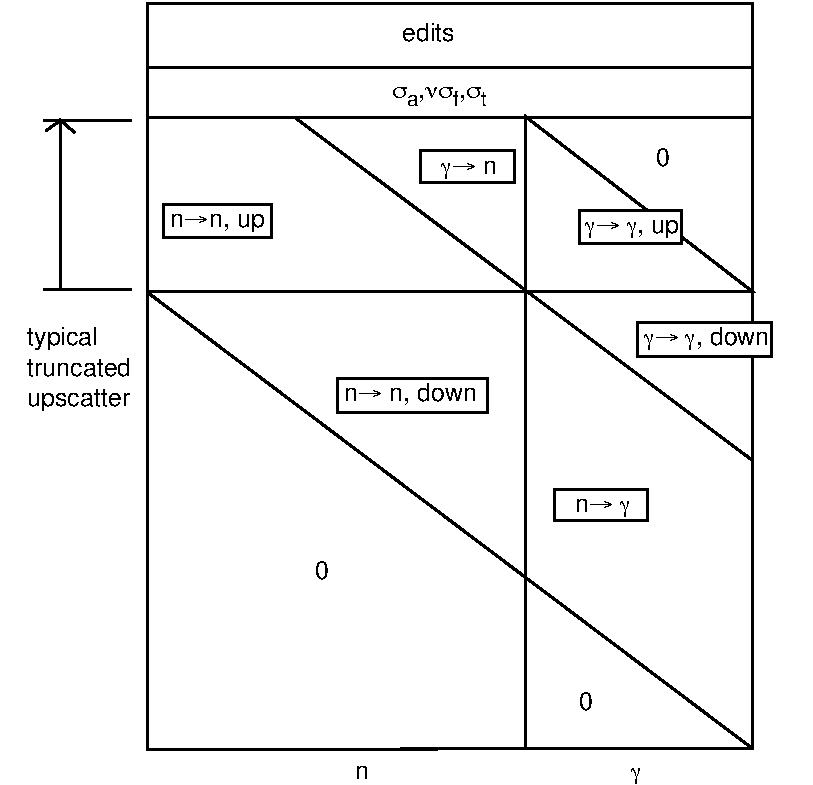
\includegraphics[keepaspectratio, height=4.6in, angle=0]{figs/groupr3}
\caption[Coupled Neutron/Photon Tables]{Arrangement of neutron (n) and
 photon ($\gamma$) cross sections in a coupled transport table.  The group
 index increases from left to right, and the position index increases from top
 to bottom.  The $\gamma{\rightarrow}$n and $\gamma{\rightarrow}\gamma$
 upscatter blocks are normally empty.}
\label{gr3}
\end{figure}

\subsection{Thermal Data}
\label{ssGROUPR_Thermal}

GROUPR uses the thermal data written onto the PENDF tape
by the \hyperlink{sTHERMRhy}{THERMR} module\index{THERMR}.  It
does not process ENDF File-7\index{File 7}
data directly.  Three different representations of thermal scattering
are used in ENDF.

For crystalline materials like graphite, coherent elastic (with zero
energy change)\index{coherent elastic} scattering can take place.  The
cross section for this process shows well-defined Bragg
edges\index{Bragg edges} at energies that correspond to the
various lattice-plane spacings in the crystalline powder.  As shown
in \hyperlink{sTHERMRhy}{THERMR},\index{THERMR} the angular dependence of the
coherent elastic cross section can be written as

  \begin{equation}
    \sigma^{coh}(E,\mu)=\sum_i {{b_i} \over {E}}
    \,\delta(\mu-\mu_i)\,\,,
  \label{Eq64}
  \end{equation}

\noindent
where

  \begin{equation}
    \mu_i=1-2{{E_i} \over {E}}\,\,,
  \end{equation}

\noindent
and where the $E_i$ are the energies of the Bragg
edges.  \hyperlink{sTHERMRhy}{THERMR}
integrates Eq.~\ref{Eq64} over all angles, and writes the result
to the PENDF tape.  Clearly, the $b_i$ can be recovered from

  \begin{equation}
    E\,\sigma^{coh}(E)=\mathop{{\sum}'}_i b_i\,\,,
  \label{Eq66}
  \end{equation}
\vspace{1 pt}

\noindent
where the primed sum is over all $i$ such that $E_i <E$.  It is only
necessary to locate the steps in $E\,\sigma^{coh}(E)$.  The size of the
step gives $b_i$, and the $E$ for the step gives $E_i$.  The Legendre
cross sections become

  \begin{equation}
    \sigma^{coh}_\ell (E)=\mathop{{\sum}'}_i {{b_i} \over {E}}
     P_\ell (\mu_i)\,\,,
  \label{Eq67}
  \end{equation}

\noindent
where any terms with $\mu_i{<}-1$ are omitted from the primed sum.
An example of a pointwise cross section for coherent elastic scattering
is given in Fig.~\ref{gr4}.

\begin{figure}[thb]\centering
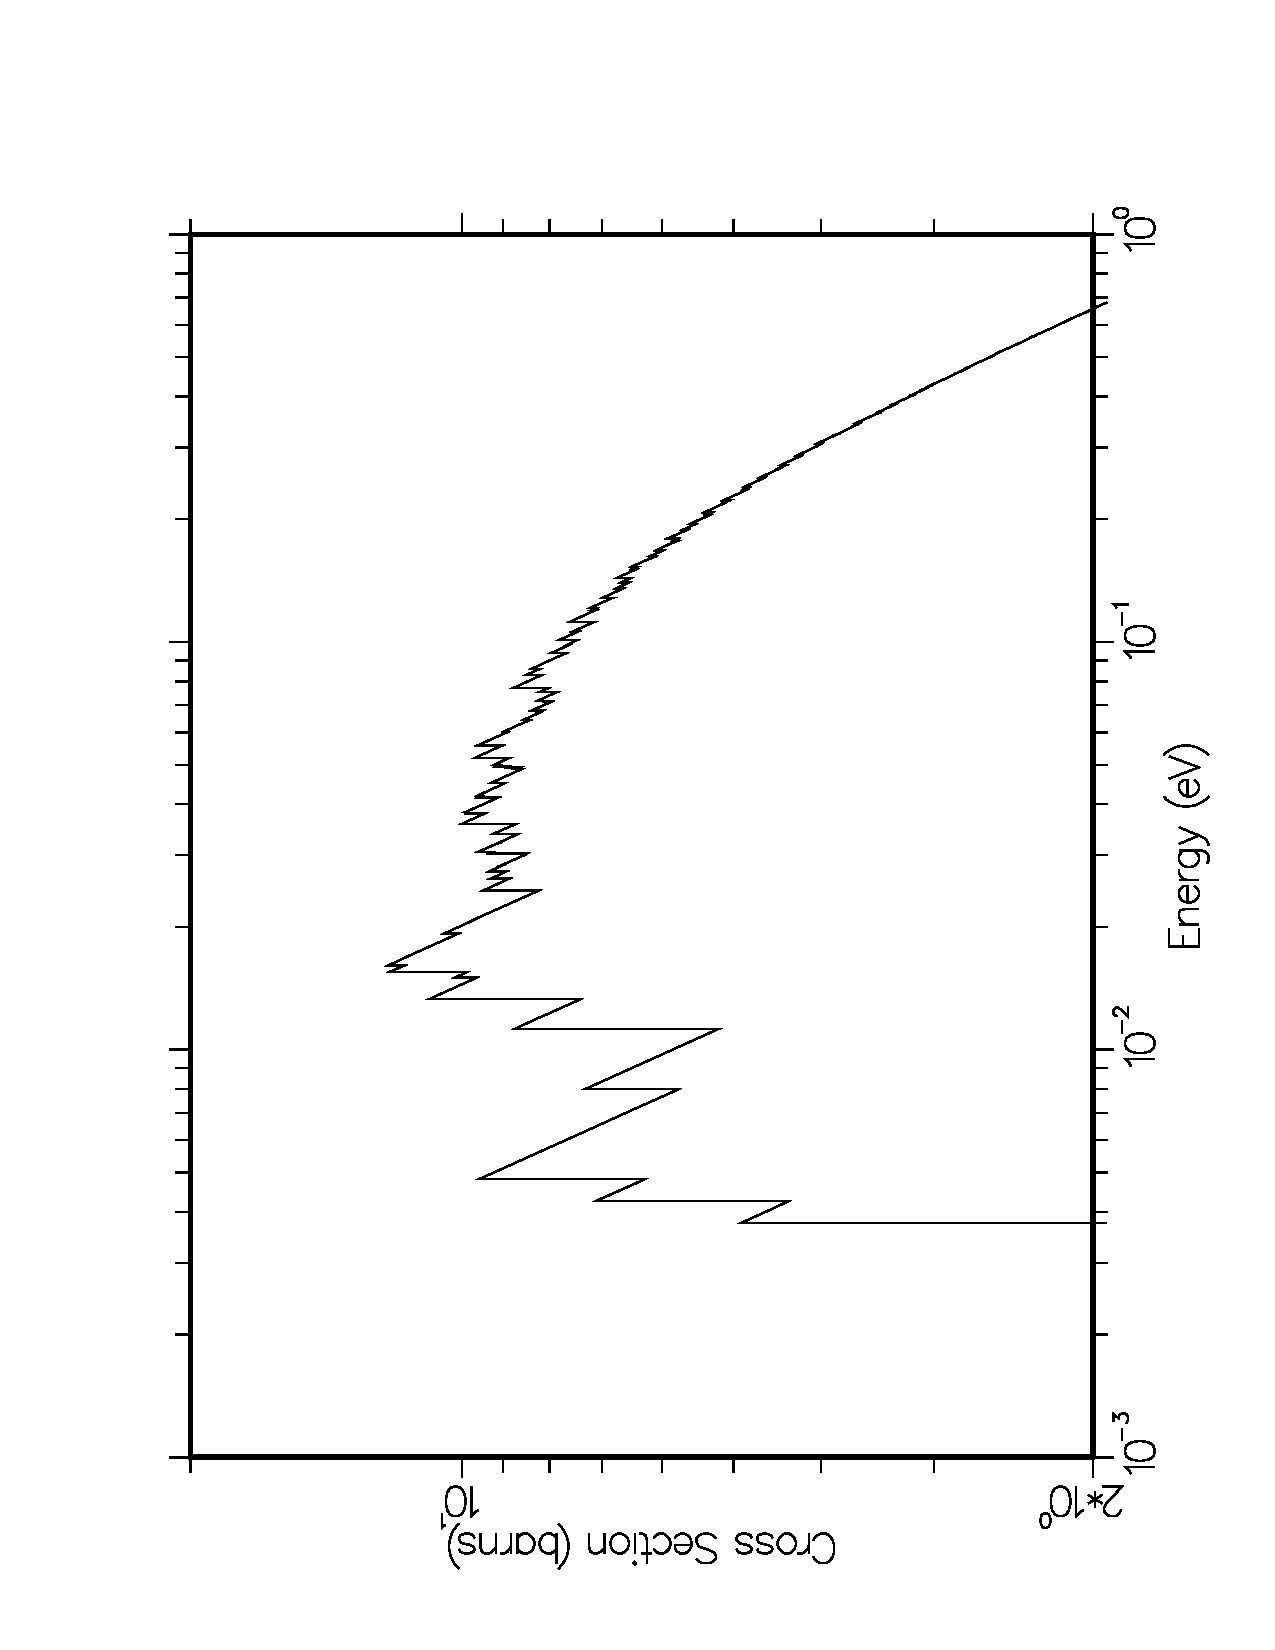
\includegraphics[keepaspectratio, height=3.5in, angle=270]{figs/groupr4ack}
\caption[Bragg edges seen in the BeO coherent elastic scattering cross section]
{The coherent elastic scattering cross section for BeO showing the Bragg edges.
 The shape of $\sigma(E)$ between edges is $1/E$.  Therefore, the function
 $E\sigma(E)$ is a stair-step function, where the height of each step depends
 on the structure factor for
 scattering from that set of lattice planes (see Eq.~\ref{Eq66}).}
\label{gr4}
\end{figure}

For hydrogenous solids like polyethylene and zirconium hydride, the
process of incoherent elastic scattering\index{incoherent elastic}
is important.  Here the angular cross section is given by

  \begin{equation}
    \sigma^{iel}(E,\mu)={{\sigma_b}\over 2}
    \exp \biggl[ -{{2EW}\over A} (1-\mu) \biggr]\,\,.
  \end{equation}
\vspace{0.5 pt}

\noindent
\hyperlink{sTHERMRhy}{THERMR} converts this into
an integrated cross section, $\sigma^{iel}(E)$, and a set of $N$
equally probable emission cosines, $\overline{\mu}_i$.  These angles
are present in File 6 on the PENDF tape.  GROUPR can easily determine
the Legendre components of the scattering cross section using

  \begin{equation}
    \sigma^{iel}_{\ell} (E)=\sigma^{iel}(E)
    {{1}\over {N}} \sum_{i=1}^N P_{\ell} (\mu_i )\,\,.
  \label{Eq69}
  \end{equation}

The third thermal process is incoherent inelastic scattering.
\index{incoherent inelastic} Here the neutron energy can either
increase or decrease.  The data from
\hyperlink{sTHERMRhy}{THERMR} are given as a
cross section in File 3 and an energy-angle distribution
using a special form of File 6.  The distribution is
represented by sets of secondary-energy values $E'$ for particular
incident energies $E$.  For each $E{\rightarrow}E'$, a scattering
probability $f^{inc} (E{\rightarrow}E')$ and a set of equally probable
cosines $\mu_i (E{\rightarrow}E')$ are given.  The scattering probabilities
for each value of $E$ integrate to unity.  Although the thermal
scattering cross section is a smooth function of incident neutron energy,
this is not true for the scattering from $E$ to one particular final
energy group $g'$, since the differential cross section tends to peak
along the line $E'{=}E$ and at energy-transfer values corresponding
to well-defined excitations in the molecule or lattice.  If interpolation
between adjacent values of $E$ were to be performed along lines of
constant $E'$, the excitation peaks and the $E{=}E'$ feature would
produce double features in the intermediate spectrum, as shown in
Fig.~\ref{gr5}.  To avoid this problem, while still using a
relatively sparse incident energy grid, GROUPR interpolates between
$E$ and $E'$ along lines of constant energy transfer.  Of course, this
breaks down at low values of $E'$, because one of the spectra will go
to zero before the other one does.  In this range, GROUPR transforms
the low-energy parts of the two spectra onto a ``unit base,'' combines
them in fractions that depend on $E$, and scales the result back out
to the interpolated value of $E'$ corresponding to $E$.

\begin{figure}[tp]\centering
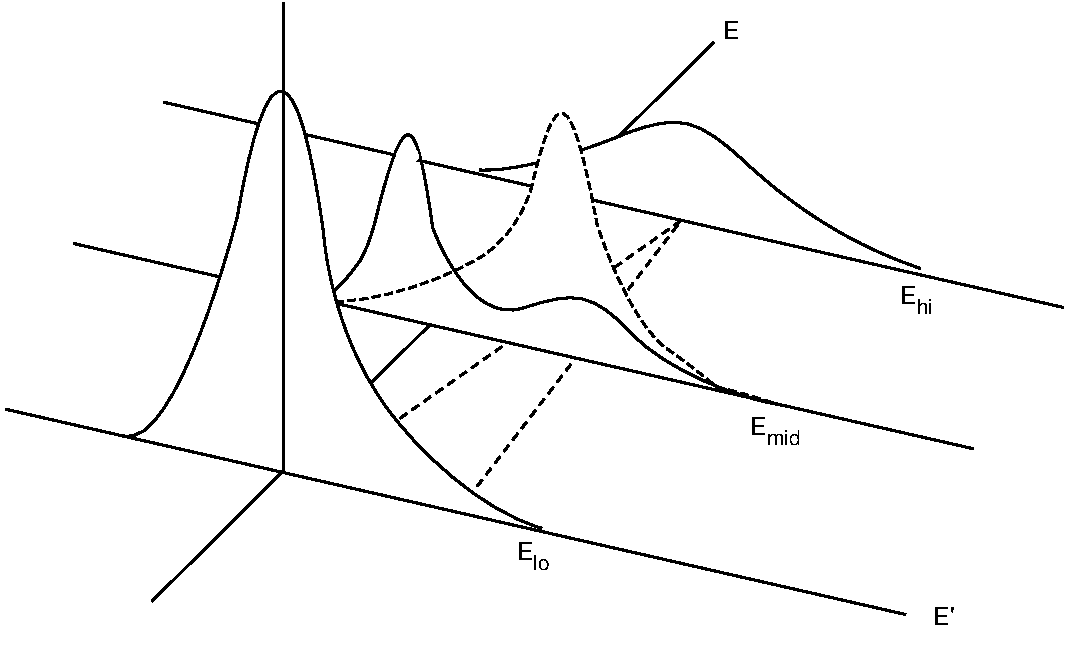
\includegraphics[keepaspectratio, height=3.25in, angle=0]{figs/groupr5}
\caption[Interpolation along lines of constant energy transfer]{Illustration of
 thermal interpolation showing the double-humped curve resulting from simple
 Cartesian interpolation for a discrete excitation (solid) and the more
 realistic curve obtained by interpolating along lines of constant energy
 transfer (dashed).}
\label{gr5}
\end{figure}

\subsection{Generalized Group Integrals}
\label{ssGROUPR_GrpInt}

In order to unify many formerly different processing tasks, GROUPR uses
the concept of a generalized group integral
  \begin{equation}
    \sigma_g={\displaystyle{\int_g {\cal F}(E)\,\sigma(E)\,\phi(E)\,dE}
    \over\displaystyle{\int_g\phi(E)\,dE}}\,\,,
  \label{Eq70}
  \end{equation}
where the integrals are over all initial neutron energies in group $g$,
$\sigma(E)$ is a cross section at $E$, and $\phi(E)$ is an estimate of
the flux at $E$.  The function ${\cal F}(E)$ is called the ``feed function''.
\index{feed function}
It alone changes for different data types.  To average a neutron cross
section, ${\cal F}$ is set to 1.  To average a ratio quantity like
$\overline \mu$ with respect to elastic scattering, ${\cal F}$ is set
to $\overline \mu$.  For photon production, ${\cal F}$ is the photon yield.
For matrices, ${\cal F}$ is the  $\ell$-th Legendre component of
the normalized probability of scattering into secondary energy group
$g'$ from initial energy $E$.  This definition is clearly independent of
whether the secondary particle is a neutron or a photon.

The question of integration grid or quadrature scheme is important for
the evaluation of Eq.~\ref{Eq70}.  Each factor in the integrands has its
own characteristic features, and it is important to account for them all.
First, a grid must be established for each factor.  As an example, the
grid of $\sigma(E)$ is generated in
\hyperlink{sRECONRhy}{RECONR}\index{RECONR} such
that sigma can be obtained to within a given tolerance by
linear interpolation.  GROUPR contains a subroutine
\cword{getsig}\index{getsig@{\ty getsig}} which carries out this
interpolation at $E$ and also returns the next grid energy in
\cword{enext}.  Subroutines \cword{getflx}\index{getflx@{\ty getflx}}
and \cword{getff}\index{getff@{\ty getff}} perform similar functions
for the flux and feed function.  It is now easy to generate a
union grid for the three-factor integrand using the following Fortran:

\small
\begin{ccode}
       ...
      call getsig(e,enext,...)
      call getflx(e,en,...)
      if (en.lt.enext) enext=en
      call getff(e,en,...)
      if (en.lt.enext) enext=en
       ...
\end{ccode}
\normalsize

\noindent
On occasion, there will be a discontinuity at \cword{enext} for one of the
factors.  In order to flag such a case, each ``\cword{get}'' routine
also sets a discontinuity flag \cword{idisc}.  The grid logic actually
used throughout NJOY is as follows:

\small
\begin{ccode}
     ...
      call getsig(e,enext,idisc,...)
      call getflx(e,en,idis,...)
      if (en.eq.enext.and.idis.gt.idisc) idisc=idis
      if (en.lt.enext) idisc=idis
      if (en.lt.enext) enext=en
      call getff(e,en,idis,...)
      if (en.eq.enext.and.idis.gt.idisc) idisc=idis
      if (en.lt.enext) idisc=idis
      if (en.lt.enext) enext=en
      ...
\end{ccode}
\normalsize

\noindent
This union grid for the integrand in the numerator is used to subdivide
the generalized group integral of Eq.~\ref{Eq70} into ``panels''.  The
main program of GROUPR carries out the integrals with the following logic:

\small
\begin{ccode}
      ...
      elo=egn(ig)
      ehi=egn(ig+1)
      enext=ehi
  230 call panel(elo,enext,...)
      if (enext.eq.ehi) go to 240
      elo=enext
      enext=ehi
      go to 230
  240 continue
      ...
\end{ccode}
\normalsize

\noindent
A panel is first defined by the energy bounds of group $g$.  Subroutine
\cword{panel} is called to sum in the contributions from this panel.
However, \cword{panel} discovers that the integrand has a grid point at
\cword{enext} less than \cword{ehi}.  It adds in the contributions for
the smaller panel \cword{elo} to \cword{enext} and returns.  GROUPR now
sees that \cword{enext} is less than \cword{ehi}, so it tries a new panel
from the top of the last panel (\cword{elo}=\cword{enext}) to \cword{ehi}.
This loop continues until a panel with \cword{ehi} as its upper bound
is summed in.  The integral for this group is then complete.

In this simple way, the algorithm accounts for the user's group
structure and for all structure in the integrand.  The method used for
establishing the \hyperlink{sRECONRhy}{RECONR} grid
makes this integration algorithm
equivalent to adaptive integration as used in MINX\cite{MINX}.
It has the great advantage that no ``stack'' of intermediate results
is carried along.  This single-pass feature of the quadrature scheme
allows many different integrals to be accumulated simultaneously
within reasonable storage limits.  In this way, GROUPR accumulates
cross sections for all values of $\sigma_0$ simultaneously.  Similarly,
group-to-group cross sections are computed for all secondary energy
groups and all Legendre orders simultaneously.

Any degree of complexity can be used for the integral over each subpanel.
Because $\sigma(E)$ has been linearized, \cword{panel} is based on
trapezoidal integration.  Both $\phi(E)$ and
$R(E)=\sigma(E){\times}\phi(E)$ are assumed to vary linearly across each
panel.  In some cases, the feed function is oscillatory over a certain
energy range (see Two-Body Scattering, Section~\ref{ssGROUPR_TwoBody}).
It is then convenient to integrate inside the panel using Lobatto
quadrature\cite{ref13}\index{Lobatto quadrature} (note the variable
\cword{nq} in \cword{panel}\index{panel@{\ty panel}}).  As discussed
in more detail later, this method can obtain accurate results
for an oscillatory function whose integral is small with respect to its
magnitude.  This behavior is characteristic of the higher Legendre
components of two-body scattering cross sections.

The generalized integration scheme discussed here is also used by
the \hyperlink{sGAMINRhy}{GAMINR}\index{GAMINR}
and \hyperlink{sERRORRhy}{ERRORR}\index{ERRORR} modules.

\subsection{Two-Body Scattering}
\label{ssGROUPR_TwoBody}

Elastic scattering (ENDF/B MT=2) and discrete inelastic neutron
scattering (with MT=51 -- 90) are both examples of two-body kinematics
\index{two-body kinematics} and are treated together by GROUPR.  Some
other cases that occur for charged particles or in
File 6\index{File 6} will be discussed later.  The
feed function required for the group-to-group matrix calculation
may be written

  \begin{equation}
    {\cal F}_{\ell g'}(E)=\int_{g'}dE'\,\int_{-1}^{+1}d\omega\,
    f(E{\rightarrow}E',\omega)\,P_{\ell}(\mu[\omega])\,\,,
  \label{Eq71}
  \end{equation}

\noindent
where $f(E{\rightarrow}E',\omega)$ is the probability of scattering
from $E$ to $E'$ through a center-of-mass cosine $\omega$ and $P_{\ell}$
is a Legendre polynomial for laboratory cosine $\mu$.  The laboratory
cosine corresponding to $\omega$ is given by

  \begin{equation}
    \mu={{1+R\omega}\over
    {\sqrt{1+R^2+2R\omega }}}\,\,,
  \label{Eq72}
  \end{equation}

\noindent
and the cosine $\omega$ is related to secondary energy $E'$ by

  \begin{equation}
    \omega={{E'(1+A)^2/A'-E(1+R^2)}
    \over{2RE}}\,\,,
  \label{Eq73}
  \end{equation}

\noindent
where $A'$ is the ratio of the emitted particle mass to the incident
particle mass ($A'{=}1$ for neutron scattering).  In Eqs.~\ref{Eq72}
and \ref{Eq73}, $R$ is the effective mass ratio

  \begin{equation}
    R=\sqrt{\frac{A(A+1-A')}{A'}}\sqrt{1-{{(A+1)(-Q)}\over{AE}} }\,\,,
  \label{Eq74}
  \end{equation}

\noindent
where $A$ is the ratio of target mass to neutron mass, and $-Q$ is the
energy level of the excited nucleus ($Q{=}0$ for elastic scattering).
Integrating Eq.~\ref{Eq71} over secondary energy gives

  \begin{equation}
    {\cal F}_{\ell g'}(E)=\int_{\omega_1}^{\omega_2}
    f(E,\omega)\,P_{\ell}(\mu[\omega])\,d\omega\,\,,
  \label{Eq75}
  \end{equation}

\noindent
where $\omega_1$ and $\omega_2$ are evaluated using Eq.~\ref{Eq73}
for $E'$ equal to the upper and lower bounds of $g'$, respectively.
The scattering probability is given by

  \begin{equation}
    f(E,\omega)=\sum_{\ell=0}^L f_{\ell}(E)\,P_{\ell}(\omega)\,\,,
  \label{Eq76}
  \end{equation}

\noindent
where the Legendre coefficients are either retrieved directly from the
ENDF File 4 or computed from File 4 tabulated angular distributions
(see subroutines \cword{getfle}\index{getfle@{\ty getfle}} and
\cword{getco}\index{getco@{\ty getco}}).

The integration in Eq.~\ref{Eq75} is performed (see subroutine
\cword{getdis}\index{getdis@{\ty getdis}}) simultaneously for all
Legendre components using Gaussian quadrature\cite{ref13}.
\index{Gaussian quadrature}  The quadrature order is selected
based on the estimated polynomial order of the integrand.  A
reasonable estimate is given by

  \begin{equation}
    {\rm ND} + {\rm NL} +\log(300/A)\,\,,
  \label{Eq77}
  \end{equation}

\noindent
where ND is the number of Legendre components desired for the feed
function, and NL is the number of components required to represent
$f(E,\omega)$.  The log term approximates the number of additional
components required to represent the center-of-mass to lab transformation.

The two-body feed function for higher Legendre orders is a strongly
oscillatory function in some energy ranges.  An example is shown in
Fig.~\ref{gr6}.  Furthermore, the integral of the oscillatory part
is often small with respect to the magnitude of the function.  Such
functions are very difficult to integrate with adaptive techniques,
which converge to some fraction of the integral of the absolute value.
This is the reason that MINX\cite{MINX}\index{MINX} gave poor answers
for small Legendre components of the scattering matrix.  Gaussian methods,
on the other hand, are capable of integrating such oscillatory functions
exactly if they are polynomials.  Since a polynomial representation
of the feed function is fairly accurate, a Gaussian quadrature scheme
was chosen.  The scheme used is also well adapted to performing many
integrals in parallel.  In GROUPR, all Legendre components and all
final groups are accumulated simultaneously (see
\cword{panel}\index{panel@{\ty panel}}).

\begin{figure}[t]\centering
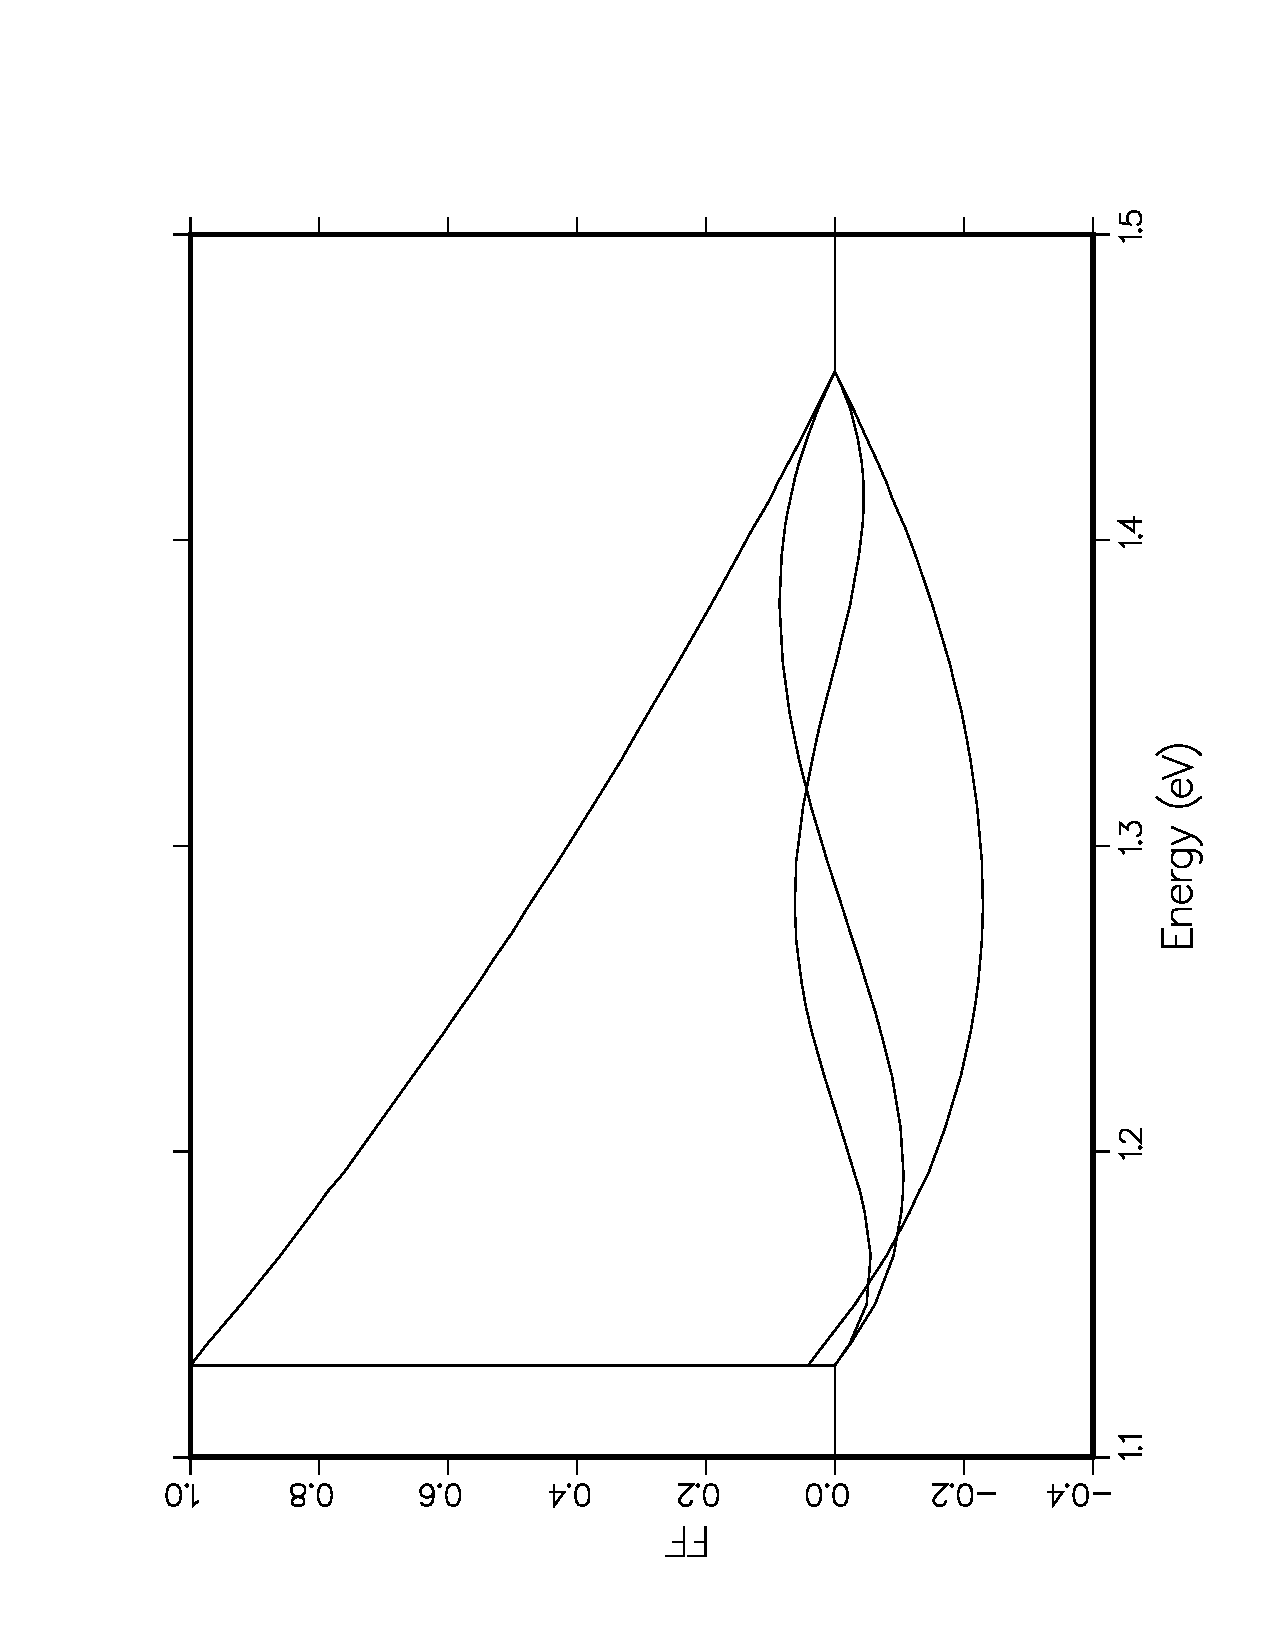
\includegraphics[keepaspectratio, height=3.5in, angle=-90]{figs/groupr6ack}
\caption[Sample two-body scattering feed function]{A typical feed
function for two-body scattering showing the oscillations that must
be treated correctly by the integration over incident energy.}
\label{gr6}
\end{figure}

The boundaries of the various regions of the feed function are
called ``critical points.''\index{critical points}  Between critical
points, the feed function is a smooth analytic function of
approximately known polynomial order.  It is only necessary
to add these critical points to the incident energy grid of
the feed function (the \cword{enext} variable) and to tell
\cword{panel}\index{panel@{\ty panel}} what quadrature order
(\cword{nq}) to use.  The critical points are determined in
\cword{getff}\index{getff@{\ty getff}} by solving Eq.~\ref{Eq73} for
the values of $E$ for which $\omega=+1$ and $\omega=-1$ when $E'$ is
equal to the various group boundaries.  This can be done by writing

  \begin{equation}
    {{E_g}\over{E}}=
    {{1}\over{(1+A)^2}}\bigl[ R^2\pm 2R+1\bigr]\,\,,
  \end{equation}
\vspace{0.5 pt}

\noindent
substituting for $E$ using Eq.~\ref{Eq74}, and then solving
for $R$.  The result is

  \begin{equation}
    E_{crit}={\displaystyle{ {{(A+1)(-Q)}\over{A}} }\over
    \displaystyle{1- {\displaystyle{A'F^2}\over{A(A+1-A')}} }}\,\,,
  \label{Eq79}
  \end{equation}
\vspace{0.5 pt}

\noindent
where
  \begin{equation}
    F={{1\pm\sqrt{D}}\over{1+ \displaystyle{{E_F}\over{(-Q)}} }}\,\,,
  \end{equation}
\vspace{0.5 pt}

  \begin{equation}
    D=\biggl[ \frac{A(A+1-A')}{A'}
       \biggl( 1+{{E_F}\over{(-Q)}} \biggr) -1 \biggr]
    {{E_F}\over{(-Q)}}\,\,,
  \end{equation}
\vspace{0.5 pt}

\noindent
and
  \begin{equation}
    E_F={{1+A}\over {A+1-A'}} E_g\,\,.
  \label{Eq82}
  \end{equation}

File 4 can also contain angular distributions for charged-particle
emission through discrete levels (for ENDF/B-VI and later see
MT=600 -- 648 for protons,
MT=650 -- 698 for deuterons, and so on; the elastic case, MT=2, is
discussed in the next section).  Moreover, File 6 can contain angular
distributions for discrete two-body scattering (see Law 3).  It can
also declare that a particular particle is the recoil particle
from a two-body reaction (Law 4), in which case the appropriate
angular distribution is obtained from the corresponding Law 3
subsection by complementing the angle.  The representation of the
angular distribution for these laws is almost identical to that
in File 4, and the calculation is done in
\cword{getdis}\index{getdis@{\ty getdis}} using much
of the File 4 coding.  The effects on the kinematics of the difference
in the mass of the emitted and incident particles are handled by the
variable $A'$ in the above equations.

\subsection{Charged-Particle Elastic Scattering}
\label{ssGROUPR_CPEl}

Coulomb scattering\index{Coulomb scattering} only occurs in the
elastic channel, and this calculation also uses the
\cword{getdis} subroutine.  The problem with Coulomb scattering
is that the basic Rutherford formula\index{Rutherford formula}
becomes singular at small angles.  In practice, this singularity
is removed by the screening effects of the atomic electrons.
\index{atomic screening}  The forward transport of charged
particles in this screening regime is usually handled by
continuous-slowing-down theory by using a ``stopping power''.
\index{stopping power}
The new ENDF-6 format allows for three different ways to handle the
large-angle scattering regime.  First and most general is the nuclear
amplitude expansion:\index{nuclear amplitude expansion}

\begin{eqnarray}
   \sigma&=&|{\rm nucl} + {\rm coul}|^2\nonumber\\
         &=& \sigma_{\rm nucl}+\sigma_{\rm coul}+{\rm interference}
\end{eqnarray}

\noindent
The Coulomb term is given by the Rutherford formula, a Legendre
expansion is defined for the nuclear term, and a complex Legendre
expansion is defined for the interference term.  This representation
cannot be generated directly from experimental data; an R-matrix
or phase-shift analysis is necessary.

A method very closely related to experiment ($\sigma_{\rm exp}$) is the
nuclear plus interference (NI) formula:
\index{nuclear plus interference}

\begin{equation}
   \sigma_{\rm NI}(\mu,E)=\sigma_{\rm exp}(\mu,E)
      -\sigma_{\rm coul}(\mu,E),
\end{equation}

\noindent
where the function is only defined for angles with cosines
$\mu{<}\mu_{\rm max}$.  The minimum angle is usually taken to be
somewhere around 20 degrees (GROUPR uses $\mu_{\rm max}{=}0.96$).
This function is still ill-behaved near the cutoff, and it must be
tabulated.  The third option is the residual cross section expansion:
\index{residual cross section expansion}

\begin{equation}
   \sigma_R(\mu,E)=(1-\mu)\bigl[\sigma_{\rm exp}(\mu,E)
      -\sigma_{\rm coul}(\mu,E)\bigr].
\end{equation}

\noindent
The $(1-\mu)$ term removes the pole at the origin.  The residual is
uncertain, but it is usually small enough that the entire curve can be
fitted with Legendre polynomials without worrying about what happens at
small angles.   In practice, both the nuclear amplitude expansion and
the nuclear plus interference representation are converted to the
residual cross section representation in subroutine
\cword{conver}\index{conver@{\ty conver}}.  As a result,
\cword{getdis}\index{getdis@{\ty getdis}} only has to cope with
the one representation.


\subsection{Continuum Scattering and Fission}
\label{ssGROUPR_Continuum}

In ENDF evaluations, scattering from many closely-spaced levels or
multibody scattering such as (n,2n), (n,n$'\alpha$) or fission is often
represented using a separable function of scattering cosine and
secondary neutron energy

  \begin{equation}
    f(E{\rightarrow}E',\mu)=F(E,\mu)\,g(E{\rightarrow}E')\,\,,
  \label{Eq83}
  \end{equation}

\noindent
where $F$ is the probability that a neutron will scatter through a
laboratory angle with cosine $\mu$ irrespective of final energy $E'$.  It is
obtained from MF=4.  Similarly, $g$ is the probability that a neutron's
energy will change from $E$ to $E'$ irrespective of the scattering angle,
and it is given in MF=5.  Continuum reactions are mostly identified by
MT numbers of 6 -- 49 and 91.  Recently, previously unused MT numbers,
152 through 200, were assigned to additional continuum reactions
that are beginning to appear in specialized evaluated files that extend
beyond 20 MeV ({\it e.g.}, the International Reactor Dosimetry and Fusion
File).  Secondary-energy distributions, whether found in MF=5 or MF=6
are represented by ``Laws" as follows:

\begin{center}
\begin{tabular}{cl}
Law & Description \\ \hline
1  & Arbitrary tabulated function \\
5  & General evaporation spectrum \\
   & (Used for delayed neutrons only.) \\
7  & Simple Maxwellian fission spectrum \\
9  & Evaporation spectrum \\
11 & Energy-dependent Watt fission spectrum \\
12 & Energy-dependent spectrum of Madland and Nix \\ \hline
\end{tabular}
\end{center}
\vspace{3 pt}

The feed functions for continuum scattering are simply

  \begin{equation}
    {\cal F}_{\ell g'}(E') = \int_{-1}^{+1} P_{\ell}(\mu) \,f(E,\mu)\,d\mu
    \int_{g'} g(E,E')\,dE'\,\,.
  \end{equation}
\vspace{0.5 pt}

\noindent
The first integral is returned by \cword{getfle} [``fle'' for $f_\ell (E)$]
as described above, and the second integral is returned by \cword{getsed}
(``sed'' for secondary-energy distribution).

For Law 1, $g$ is given as a tabulated function of $E'$ for various
values of E.  When $E_1\leq E<E_2$, the term $\int_{g'} g(E,E')\,dE'$ is
obtained by interpolating between precomputed values of
$\int_{g'} g(E_1,E')\,dE'$ and $\int_{g'} g(E_2,E')\,dE'$ in subroutine
\cword{getsed}.  Except in the case of fission, any apparent upscatter
produced by the ``stairstep'' treatment near $E{=}E'$ is added to the
in-group scattering term ($g'{=}g$).

For Law 5, $g(x)$ is given versus $x=E'/\theta(E)$ and $\theta(E)$
is given vs. E in File 5.  This secondary neutron distribution leads to
the following group integral:

  \begin{equation}
    \int_{g'}g(E,E')\,dE'=\theta(E)
    \int_{E_1/\theta}^{E_2/\theta}g(x)\,dx\,\,,
  \end{equation}
\vspace{0.5 pt}

\noindent
with $E_1$ and $E_2$ being the lower and upper boundary energies
for group $g'$.

For Law 7, the secondary-energy distribution is given by

  \begin{equation}
    g(E,E')={{\sqrt{E'}}\over I} \exp \biggl( {-{{E'}
    \over{\theta(E)}}} \biggr) \,\,,
  \label{Eq86}
  \end{equation}
\vspace{0.5 pt}

\noindent
where the effective temperature $\theta(E)$ is tabulated in File 5
and the normalization factor is given by

  \begin{equation}
    I=\theta^{3/2} \bigl[ {\sqrt{\pi \over 4}}
    {\,\rm erf}(x) - x e^{-x} \bigr]\,\,,
  \end{equation}
\vspace{0.5 pt}

\noindent
where

  \begin{equation}
    x={{E-U}\over \theta}\,\,.
  \label{Eq88}
  \end{equation}
\vspace{0.5 pt}

\noindent
Here $U$ is a constant used to define the upper limit of secondary
neutron energy $\theta \le E' \le E{-}U$.  The desired group integral
is given by

  \begin{eqnarray}
    \int_{g'}g(E,E')\,dE'&=&
    \int_{E_1}^{E_2}g(E,E')\,dE'\nonumber\\
    &=& {{X_1-X_2-Y_1+Y_2}\over{\sqrt{\pi/4}-Y-X}}\,\,,
  \label{Eq89}
  \end{eqnarray}

\noindent
where

  \begin{equation}
    X=\sqrt{x}\,e^{-x}\,\,,
  \end{equation}

  \begin{equation}
    Y=\sqrt{\pi \over 4}\,{\rm rerfc}(\sqrt{x})\,\,,
  \end{equation}

\noindent
and where $X_1$, $Y_1$, $X_2$, and $Y_2$ refer to $X$ and $Y$
evaluated at $E_1/\theta$ and $E_2/\theta$.  The integral of
Eq.~\ref{Eq89} is computed in \cword{anased}\index{anased@{\ty anased}}
(``\cword{ana}'' for analytic).  The function ``rerfc'' is the reduced
complementary error function\cite{ref13}.

For Law 9, the secondary-energy distribution is given by

  \begin{equation}
    g(E,E')={{E'}\over{I}}\exp \biggl(-{{E'}\over{\theta(E)}} \biggr)\,\,,
  \end{equation}

\noindent
where

  \begin{equation}
    I=\theta^2 \bigl[ 1-e^{-x}(1+x) \bigr]\,\,.
  \end{equation}

\noindent
Here $x$ has the same meaning as above -- see Eq.~\ref{Eq88}.  The
group integral is

  \begin{equation}
    \int_{g'}g(E,E')\,dE'={{(1+x_1)e^{-x_1}-(1+x_2)e^{-x_2}}
    \over{1-(1+x)e^{-x}}}\,\,,
  \end{equation}

\noindent
where $x_1$ and $x_2$ refer to $E_1/\theta$ and $E_2/\theta$, respectively.
This result is also computed in \cword{anased}.

For Law 11, the secondary-energy distribution is given by

  \begin{equation}
    g(E,E')={{e^{-E'/a}}\over I}\sinh\bigl(\sqrt{bE'}\bigr)\,\,,
  \end{equation}

\noindent
where

  \begin{equation}
    I={1\over 2} \sqrt{{{\pi a^3 b}\over 4}}
    \,e^{x_0} \bigl[ {\rm erf}(\sqrt{x}-\sqrt{x_0})
    +{\rm erf}(\sqrt{x}+\sqrt{x_0}) \bigr]
    -a e^{-x\sinh(abx)}\,\,.
  \end{equation}

\noindent
In this case, $a(E)$ and $b(E)$ are given in File 5,

  \begin{equation}
    x={{E-U}\over a}\,\,,
  \end{equation}
\vspace{0.5 pt}

\noindent
and

  \begin{equation}
    x_0={{ab}\over 4}\,\,.
  \end{equation}
\vspace{0.5 pt}

\noindent
The group integrals are given by

  \begin{equation}
    \int_{g'}g(E,E')={{H(x_1,x_2,x_0)}\over{H(0,x,x_0)}}\,\,,
  \label{Eq99}
  \end{equation}
\vspace{0.5 pt}

\noindent
where

  \begin{eqnarray}
    H(x_1,x_2,x_0)&=&H_2(\sqrt{x_1}-\sqrt{x_0},\sqrt{x_2}-\sqrt{x_0})\nonumber\\
    &+&\sqrt{x_0}H_1(\sqrt{x_1}-\sqrt{x_0},\sqrt{x_2}-\sqrt{x_0})\nonumber\\
    &-&H_2(\sqrt{x_1}+\sqrt{x_0},\sqrt{x_2}+\sqrt{x_0})\nonumber\\
    &+&\sqrt{x_0}H_1(\sqrt{x_1}+\sqrt{x_0},\sqrt{x_2}+\sqrt{x_0})\,\,,
  \end{eqnarray}

\noindent
and where

  \begin{equation}
    H_n(a,b)={1\over\pi}\int_a^b z^n e^{-z^2}\,dz\,\,.
  \end{equation}
\vspace{0.5 pt}

\noindent
The methods for computing $H_n$ are described in
\hyperlink{sBROADRhy}{BROADR}.  When $\sqrt{x_2}<.01$, a
short-cut calculation can be used
for the numerator of Eq.~\ref{Eq99}

  \begin{equation}
    {{4\sqrt{x_0}e^{-x_0}}\over{3\sqrt{\pi /4}}}
    \bigl[ x_2^{3/2}-x_1^{3/2} \bigr]\,\,.
  \end{equation}
\vspace{0.5 pt}

For Law 12, the Madland-Nix option, the secondary-energy
\index{Madland-Nix law}
distribution is given by

  \begin{equation}
    g(E,E')={1 \over 2} \bigl[ G(E',E_{fl})+G(E',E_{fh}) \bigr]\,\,,
  \end{equation}

\noindent
where

  \begin{eqnarray}
    \lefteqn{G(E',E_f)}\nonumber\\
    & & ={{1}\over {3\sqrt{E_fT_m}}}
    \biggl[ u_2^{3/2}E_1(u_2)-u_1^{3/2}E_1(u_1)
    +\gamma (3/2,u_2)-\gamma (3/2,u_1) \biggr]\,\,,\nonumber\\
    \mbox{ }
  \end{eqnarray}

  \begin{equation}
    u_1=(\sqrt{E'}-\sqrt{E_f})^2 / T_m\,\,,\;\hbox{and}
  \end{equation}

  \begin{equation}
    u_2=(\sqrt{E'}+\sqrt{E_f})^2 / T_m\,\,,
  \end{equation}

\noindent
and where $E_{fl}$, $E_{fh}$, and $T_m(E)$ are given in File 5.
The special functions used are the first-order exponential integral,
$E_1(x)$, and the incomplete gamma function, $\gamma (n,x)$.
The group integrals of this function are very complex\cite{ref14}.  Let

  \begin{eqnarray}
    \alpha &=& \sqrt{T_m}\,\,,\\
    \beta &=& \sqrt{E_f}\,\,,\\
    A&=& {{(\sqrt{E_1}+\beta )^2} \over {\alpha^2}}\,\,,\\
    B&=& {{(\sqrt{E_2}+\beta )^2} \over {\alpha^2}}\,\,,\\
    A'&=& {{(\sqrt{E_1}-\beta )^2} \over {\alpha^2}}\,\,,\;\hbox{and}\\
    B'&=& {{(\sqrt{E_2}-\beta )^2} \over {\alpha^2}}\,\,.
  \end{eqnarray}

\noindent
Then the integral over the range ($E_1,E_2)$ of $G$ is given by one of the
following three expression, depending on the region of integration
in which $E_1$ and $E_2$ lie.

\footnotesize
\noindent\underbar {Region I}  ($E_1 \ge E_f, E_2 > E_f$)
\begin{eqnarray}
  \lefteqn{3\sqrt{E_fT_m} \int_{E_1}^{E_2} G(E',E_f)\,dE'}\nonumber\\
  & & =\bigl[\, ({2\over 5}\alpha^2 B^{5/2}-{1\over 2}\alpha \beta B^2)
      E_1(B)-({2\over 5}\alpha^2 A^{5/2}-{1\over 2}\alpha \beta A^2)
      E_1(A) \,\bigr]\nonumber\\
  & & -\,\bigl[\,({2\over 5}\alpha^2 {B'}^{5/2}+{1\over 2}\alpha\beta {B'}^2 )
      E_1(B')-({2\over 5}\alpha^2 {A'}^{5/2}+{1\over 2}\alpha \beta {A'}^2 )
      E_1(A') \,\bigr]\nonumber\\
  & & +\,\bigl[\, (\alpha^2 B-2\alpha \beta B^{1/2})\,\gamma(3/2,B)
      -(\alpha^2 A-2 \alpha \beta A^{1/2})\,\gamma (3/2,A) \,\bigr]
      \nonumber\\
  & & -\,\bigl[\, (\alpha^2 B'+2\alpha\beta {B'}^{1/2}\,\gamma(3/2,B')
      -(\alpha^2 A'+2\alpha\beta {A'}^{1/2})\,\gamma(3/2,A')\, \bigr]
      \nonumber\\
  & & -\,{3\over 5} \alpha^2 \bigl[\, \gamma(5/2,B)-\gamma(5/2,A)
      -\gamma(5/2,B')+\gamma(5/2,A') \,\bigr]\nonumber\\
  & & -\,{3\over 2}\alpha\beta\, \bigl[\, {\rm e}^{-B}(1+B)
      -{\rm e}^{-A}(1+A)+{\rm e}^{-B'}(1+B')-{\rm e}^{-A'}(1+A')
      \,\bigr] \,\,.\nonumber\\
  \mbox{ }
\end{eqnarray}

\noindent\underbar {Region II}  ($E_1 < E_f, E_2 \le E_f$)
  \begin{eqnarray}
  \lefteqn{3 \sqrt(E_fT_m) \int_{E_1}^{E_2} G(E',E_f)\,dE'}\nonumber\\
  & & =\bigl[\, ({2\over 5}\alpha^2 B^{5/2}-{1\over 2}\alpha\beta B^2)E_1(B)
      -({2\over 5}\alpha^2 A^{5/2}-{1\over 2}\alpha\beta A^2)E_1(A)
      \,\bigr]\nonumber\\
  & & -\,\bigl[\, ({2\over 5}\alpha^2 {B'}^2)E_1(B')-({2\over 5}\alpha^2
      {A'}^{5/2}-{1\over 2}\alpha\beta {A'}^2)E_1(A') \,\bigr]
      \nonumber\\
  & &+\,\bigl[\, (\alpha^2 B-2\alpha\beta B^{1/2})\,\gamma(3/2,B)
      -(\alpha^2 A-2\alpha\beta A^{1/2})\,\gamma(3/2,A) \,\bigr]
      \nonumber\\
  & & -\,\bigl[ (\alpha^2 B'-2\alpha\beta {B'}^{1/2}\,\gamma(3,2,B')
      -(\alpha^2 A'-2\alpha\beta {A'}^{1/2})\,\gamma(3/2,A') \,\bigr]
      \nonumber\\
  & & -\,{3\over 5}\alpha\beta\bigl[\, \gamma(5/2,B)-\gamma(5/2,A)
      -\gamma(5/2,B')+\gamma(5/2,A') \,\bigr]\nonumber\\
  & & -\,{3\over 2}\alpha\beta\,\bigl[\, {\rm e}^{-B}(1+B)
      -{\rm e}^{-A}(1+A)-{\rm e}^{-B'}(1+B')+{\rm e}^{-A'}(1+A')\,\bigr]\,\,.
      \nonumber\\
  & &\mbox{ }
\end{eqnarray}

\noindent\underbar {Region III}  ($E_1 < E_f, E_2 > E_f$)
\begin{eqnarray}
  \lefteqn{3\sqrt{E_fT_m} \int_{E_1}^{E_2} G(E',E_f)\,dE'}\nonumber\\
  & & =\bigl[\, ({2\over 5}\alpha^2 B^{5/2}-{1\over 2}\alpha\beta B^2)E_1(B)
      -({2\over 5}\alpha^2 A^{5/2}-{1\over 2}\alpha\beta A^2)E_1(A)
      \,\bigr]\nonumber\\
  & & -\,\bigl[\,({2\over 5}\alpha^2 {B'}^{5/2}+{1\over 2}\alpha\beta {B'}^2)
      E_1(B') -({2\over 5}\alpha^2 {A'}^{5/2}-{1\over 2}\alpha\beta
      {A'}^2)E_1(A')\,\bigr]\nonumber\\
  & & +\,\bigl[\, (\alpha^2 B-2\alpha\beta B^{1/2})\,\gamma(3/2,B)
      -(\alpha^2 A-2\alpha\beta A^{1/2})\,\gamma(3,2,A)\,\bigr]
      \nonumber\\
  & & -\,\bigl[\, (\alpha^2 B'+2\alpha\beta {B'}^{1/2})\,\gamma(3/2,B')
      -(\alpha^2 A'-2\alpha\beta {A'}^{1/2})\,\gamma(3/2,A'_)\,\bigr]
      \nonumber\\
  & & -\,{3\over 5}\alpha^2\bigl[\,\gamma(5/2,B)-\gamma(5/2,A)
      -\gamma(5/2,B')+\gamma(5/2,A')\,\bigr]
      \nonumber\\
  & & -\,{3\over 2}\alpha\beta\,\bigl[\,{\rm e}^{-B}(1+B)-{\rm e}^{-A}(1+A)
      +{\rm e}^{-B'}(1+B')+{\rm e}^{-A'}(1+A')-2 \,\bigr]\,\,.
      \nonumber\\
  & & \mbox{ }
  \label{Eq115}
\end{eqnarray}
\normalsize

\subsection{File 6 Energy-Angle Distributions}
\label{ssGROUPR_F6_EA}

If the File 6 data are expressed as a continuous energy-angle distribution
(Law~1) in the laboratory system, it is fairly easy to generate the
multigroup transfer matrix.  As usual for GROUPR, the task is to calculate
the ``feed function'' (the Legendre moments for transferring to
all possible secondary-energy groups starting with incident energy $E$).
The $E'$ integration is controlled by the
\cword{getmf6}\index{getmf6@{\ty getmf6}} subroutine, which calls
\cword{f6lab}\index{f6lab@{\ty f6lab}} to generate the integrands.
This routine expects data in Law-1 format, where the looping order
is $E$, $E'$, $\mu$.  The only problems here are handling the new
ENDF-6 interpolation laws for two-dimensional tabulations (for
example, unit base) and converting tabulated angle functions for
$E{\rightarrow}E'$ into Legendre coefficients (which is done with
a Gauss-Legendre quadrature\index{Gauss-Legendre quadrature} of order $\sim8$).

If the File 6 data are given in the energy-angle form of Law 7 (where
the looping order is $E$, $\mu$, $E'$), GROUPR converts it to the Law 1
form using subroutine \cword{ll2lab}\index{ll2lab@{\ty ll2lab}}.  It
does this by stepping through an $E'$ grid that is the union of
the $E'$ grids for all the different angles given.  At each of
these union $E'$ values, it calculates the Legendre coefficients
using a Gauss-Legendre quadrature of order 8, and it checks back
to see if the preceding point is still needed to represent the
distribution to the desired degree of accuracy.  Now
\cword{getmf6}\index{getmf6@{\ty getmf6}} and
\cword{f6lab}\index{f6lab@{\ty f6lab}} can be used to complete
the calculation as above.

If the File 6 data are expressed in the CM system, or if the phase-space
option is used, more processing is necessary to convert to the LAB system.
This conversion is done for each incident energy $E$ given in the file.
The grid for laboratory secondary energy $E'_L$ is obtained by doing an
adaptive reconstruction of the emission probability $p_{L\ell}(E,E'_L)$
such that each Legendre order can be expressed as a linear-linear function
of $E'_L$.  This part is done in subroutine \cword{cm2lab}.  The values for
$p_{L\ell}(E,E'_L)$ are obtained in subroutine \cword{f6cm} by doing
an adaptive integration along the contour $E'_L{=}\hbox{\rm const}\,$ in
the $E'_C,\mu_C$ plane using $\mu_L$ as the variable of integration:

\begin{equation}
   p_{L\ell}(E,E'_L) = \int_{\mu_{\rm min}}^{+1}
      p_C(E,E'_C,\mu_C)\,P_\ell(\mu_L)\,J\,d\mu_L\,\,,
\label{yy1}
\end{equation}

\noindent
where $\mu$ is a scattering cosine and $L$ and $C$ denote the laboratory
and center-of-mass (CM) systems, respectively.  The Jacobian is given by

\begin{equation}
   J=\sqrt{\frac{E'_L}{E'_C}}=\frac{1}{\sqrt{1+c^2-2c\mu_L}}\,\,,
\label{yy2}
\end{equation}

\noindent
and the cosine transformation is given by

\begin{equation}
   \mu_C=J(\mu_L-c)\,\,.
\label{yy3}
\end{equation}

\noindent
The constant $c$ is given by

\begin{equation}
   c=\sqrt{\frac{A'}{(A+1)^2}}\sqrt{\frac{E}{E'_L}}\,\,,
\label{yy4}
\end{equation}
\vspace{0.5 pt}

\noindent
where $A$ is the ratio of the atomic weight of the target to the atomic
weight of the projectile, and $A'$ is the ratio of the atomic weight of
the emitted particle to the atomic weight of the projectile.  The
lower limit of the integral depends on the maximum possible value for
the center-of-mass (CM) secondary energy as follows:

\begin{equation}
   \mu_{\rm min}=\frac{1}{2c}\Bigl(1+c^2-\frac{E'_{C{\rm max}}}{E'_L}\Bigr),
\label{yy5}
\end{equation}

\noindent
where

\begin{equation}
   E'_{L{\rm max}}=E\Bigl(\sqrt{\frac{E'_{C{\rm max}}}{E}}+
      \sqrt{\frac{A'}{(A+1)^2}}\Bigr)^2.
\label{yy6}
\end{equation}
\vspace{0.5 pt}

\noindent
An example of the integration contours for this coordinate transformation
is given in Fig.~\ref{transform}.

\begin{figure}[thb]\centering
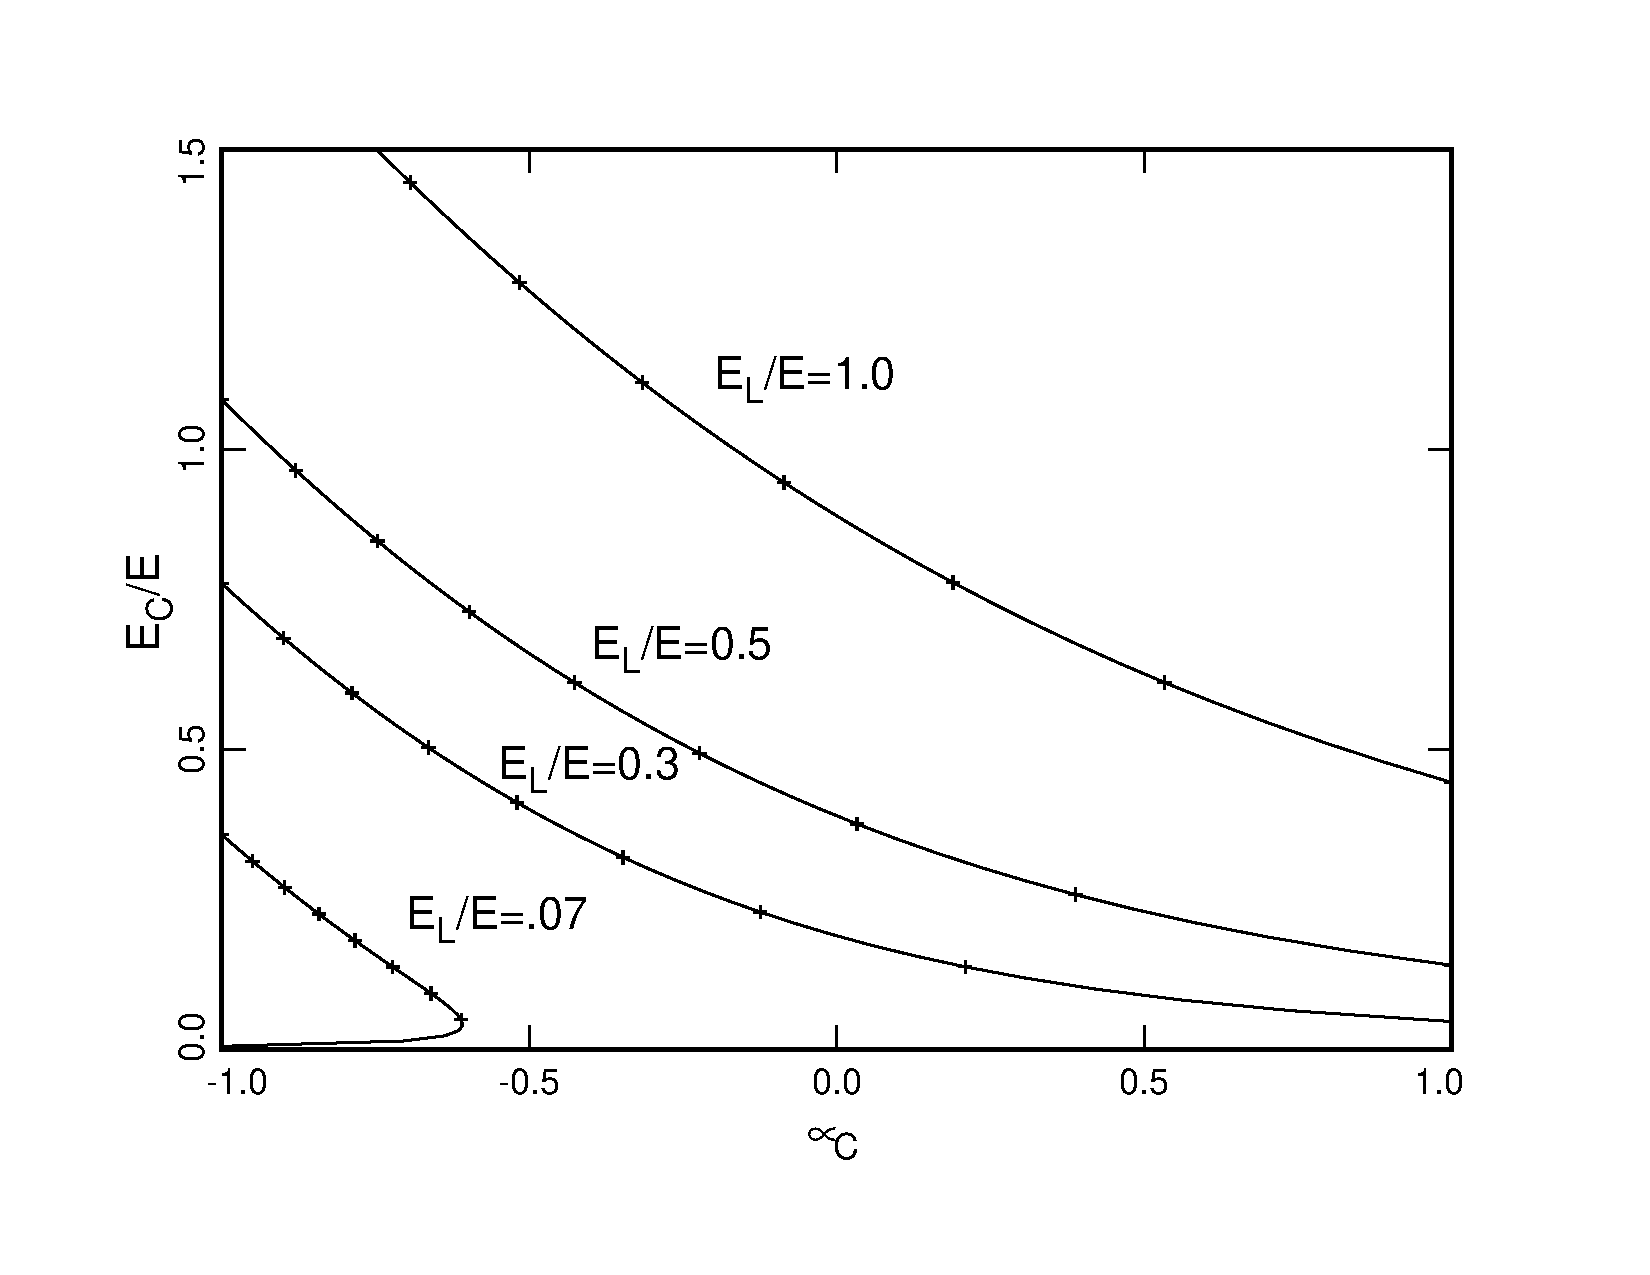
\includegraphics[keepaspectratio, height=3.5in, angle=0]{figs/groupr7ack}
\caption[Coordinate mapping between CM and LAB reference frames
 for A=2]{Coordinate mapping between CM and laboratory reference frames
 for A=2.  The parameters $E_L$ and $E_C$ are the secondary energies in the
 Lab and CM frames.  The crosses on the curves are at $\mu_L$ values of -1.0,
 -.75, -.50, \ldots, .75, and 1.0.  This figure also illustrates the advantage
 of integrating over $\mu_L$ for the contour in the lower-left corner.  The
 values of $E_C$ and $\mu_C$ are single-values functions of $\mu_L$.}
\label{transform}
\end{figure}

The CM energy-angle distribution can be given as a set of Legendre
coefficients or a tabulated angular distribution for each
possible energy transfer $E{\rightarrow}E'$, as a ``precompound fraction''
$r(E,E')$ for use with the
Kalbach-Mann\cite{km}\index{Kalbach-Mann systematics}
or Kalbach\cite{k86}\index{Kalbach systematics} angular
distributions, or as parameters for a phase-space\index{phase-space
distributions} distribution.  The first three options are processed using
\cword{f6ddx}\index{f6ddx@{\ty f6ddx}}, and the last using
\cword{f6psp}\index{f6psp@{\ty f6psp}}.  The Kalbach  option
leads to a very compact representation.  Kalbach and Mann examined
large number of experimental angular distributions for neutrons
and charged particles.  They noticed that each distribution could
be divided into two parts: an equilibrium part symmetric in $\mu$,
and a forward-peaked preequilibrium part.  The relative amount of
the two parts depended on a parameter $r$, the preequilibrium fraction,
\index{preequilibrium fraction} that varies from zero for low $E'$ to 1.0
for large $E'$.  The shapes of the two parts of the distributions
depended most directly on $E'$.  This representation is very useful
for preequilibrium statistical-model codes like
GNASH\cite{GNASH}\index{GNASH}, because they can compute the
parameter $r$, and all the rest of the angular information comes
from simple universal functions.   More specifically,
Kalbach's latest work says that

\begin{equation}
   f(\mu)=\frac{a}{2\sinh(a)}\Bigl[\cosh(a\mu)+r\sinh(a\mu)\Bigr],
\end{equation}

\noindent
where $a$ is a simple function of $E$, $E'$, and $B_b$, the separation
energy of the emitted particle from the liquid-drop model without
pairing and shell terms.  The separation energies\index{separation energy}
are computed by formulas in \cword{bach}\index{bach@{\ty bach}}.  There
is a problem for elemental evaluations, because the calculations needs
an A value for the element, and it is difficult to guess which A value
is most characteristic of the element.  A short table is included in
the routine, and an ``\cword{error in bach}'' will result if the
function is called for an element that doesn't appear
in the table.  Similar routines appear in
\hyperlink{sHEATRhy}{HEATR}\index{HEATR} and
\hyperlink{sACERhy}{ACER}\index{ACER}.  A better
long-range solution would be desirable.
Fortunately, elemental evaluations are rare in modern
evaluated libraries.

The File 6 processing methods in GROUPR apply equally well to
neutrons, photonuclear photons, and charged particles.  The effects
on the kinematics due to the difference in mass between the incident
particle and the emitted particle are handled by the variable $A'$ in
the above equations.

\subsection{Smoothing}
\label{ssGROUPR_Smooth}

For continuum CM distributions in File 6, the low-energy shape
should go like $\sqrt{E'_C}$\index{sqrt(E) shape}.  From Eq.~\ref{yy2},
we see that the low-energy shape for the Lab distribution would then go
like $\sqrt{E'_L}$.  However, ENDF/B-VII evaluations for File 6
were normally prepared using advanced nuclear model codes, such as
GNASH\index{GNASH} from LANL\index{Los Alamos National Laboratory!LANL}.  These
codes naturally produce spectra represented
with histogram bins, and these bins normally give a constant
probability from zero energy to the next bin boundary.  This
is certainly not a $\sqrt{E}$ shape!  The histogram shape can
cause trouble with the CM-Lab transformation if some care is not
taken.  Clearly, the histogram grossly overestimates the probability
of scattering to very low energies.  This apparent problem is somewhat
alleviated by the fact that the total probability of that lowest
histogram bin is usually quite small.  However, in order to get
better looking shapes, GROUPR has coding that replaces the
coarse histogram with a finer histogram chosen to represent a
$\sqrt{E}$ shape more closely.  This smoothing\index{smoothing}
coding scans up through the histogram distribution from the evaluation
to find the region that behaves like $\sqrt{E}$.  It then uses a
recursive procedure to subdivide the region using a given factor
until it reaches a fairly low energy (currently 40 eV).

A similar procedure is used to provide a $\sqrt{E}$ shape
at low energies for delayed neutron spectra.

For a few of the ENDF/B-VII\index{ENDF!ENDF/B-VII} actinides, the
energy grid used to represent the fission spectrum becomes too
coarse above 10 MeV.  If that situtation is found, GROUPR changes
the interpolation law from the given lin-lin option to
lin-log --- that is, an exponential tail is assumed for the
high energies.  This assumption is consistent with the orginal
evaluations.  This modification can be important for reaction
rates of high-threshold reactions.

These smoothing options are controlled by the global parameter
\cword{ismooth}\index{ismooth@{\ty ismooth}}, which is turned on
by default (in constrast to NJOY99 where it is turned off by default).


\subsection{GENDF Output}
\label{ssGROUPR_GENDF}

The group constants produced by GROUPR are normally written to
an output file in GENDF\index{GENDF} (groupwise ENDF) format
for use by other modules of NJOY.  For example,
\hyperlink{sDTFRhy}{DTFR}\index{DTFR}
can be used to convert a GENDF material to DTF (or ``transport'')
format; \hyperlink{sCCCCRhy}{CCCCR}\index{CCCCR} produces
the standard interface
files\cite{CCCC4} ISOTXS\index{ISOTXS}, BRKOXS\index{BRKOXS}, and
DLAYXS\index{DLAYXS}; \hyperlink{sMATXSRhy}{MATXSR}\index{MATXSR}
produces a file in MATXS\index{MATXS} format\cite{TRANSX};
and \hyperlink{sPOWRhy}{POWR}\index{POWR}
produces libraries for the Electric Power Research Institute
(EPRI)\index{EPRI} codes EPRI-CELL\index{EPRI!EPRI-CELL} and
EPRI-CPM\index{EPRI!EPRI-CPM}.  Other formats can easily be
produced by new modules, and some functions such as group collapse,
are conveniently performed directly in GENDF format.  The GENDF
format is also used for \hyperlink{sGAMINRhy}{GAMINR}\index{GAMINR}
output, and both \hyperlink{sACERhy}{ACER}\index{ACER} and
\hyperlink{sERRORRhy}{ERRORR}\index{ERRORR} use GENDF input for
some purposes.

Depending on the sign of \cword{ngout2} (see below), the GENDF file will
be written in either coded mode ({\it e.g.}, ASCII) or in the special
NJOY blocked-binary mode.  Conversion between these modes can be
performed subsequently by the
\hyperlink{sMODERhy}{MODER} module.\index{MODER}

The GENDF material begins with a header record (MF=1, MT=451), but the
format of this first section is different from MT=451 on an ENDF or
PENDF tape.  The section consists of a ``CONT'' record, containing

\begin{quote}
\centering
\begin{tabular}{ll}
\cword{ZA} &  Standard 1000*Z+A value \\
\cword{AWR} &  Atomic weight ratio to neutron \\
\cword{0} &  Zero \\
\cword{NZ} &  Number of $\sigma_0$ values \\
\cword{-1} &  Identifies a GENDF-type data file \\
\cword{NTW} &  Number of words in title
\end{tabular}
\end{quote}

\noindent
and a single ``LIST'' record, containing

\begin{quote}
\centering
\begin{tabular}{ll}
\cword{TEMPIN} &  Material temperature (Kelvin) \\
\cword{0.} &  Zero \\
\cword{NGN} &  Number of neutron groups \\
\cword{NGG} &  Number of photon groups \\
\cword{NW} &  Number of words in LIST \\
\cword{0} &  Zero \\
\cword{TITLE} &  Title from GROUPR input (\cword{NTW} words) \\
\cword{SIGZ} &  Sigma-zero values (\cword{NZ} words) \\
\cword{EGN} &  Neutron group boundaries, low to high (\cword{NGN}+1 words) \\
\cword{EGG} &  Photon group boundaries, low to high (\cword{NGG}+1 words).
\end{tabular}
\end{quote}

\noindent
For photoatomic GENDF files produced by the
\hyperlink{sGAMINRhy}{GAMINR} module, the
photon group structure is stored in \cword{ngn} and \cword{egn},
and the number of photon groups is given as \cword{ngg}=0.
The word count is NW=NTW+NZ+NGN+1+NGG+1.  The LIST record
is followed by a standard ENDF file-end record (FEND).  The normal
ENDF section-end (SEND) is omitted.

This header is followed by a series of records for reactions.
The ENDF ordering requirements are relaxed, and MF and MT values can
occur in any order.  Each section starts with a ``CONT'' record.

\begin{quote}
\centering
\begin{tabular}{ll}
\cword{ZA} &  Standard 1000*Z+A value \\
\cword{AWR} &  Standard atomic weight ratio \\
\cword{NL} &  Number of Legendre components \\
\cword{NZ} &  Number of sigma-zero values \\
\cword{LRFLAG} &  Break-up identifier flag \\
\cword{NGN} &  Number of groups
\end{tabular}
\end{quote}

\noindent
It is followed by a series of LIST records, one for every
incident-energy group with nonzero result,

\begin{quote}
\centering
\begin{tabular}{ll}
\cword{TEMP} &  Material temperature (Kelvin) \\
\cword{0.} &  Zero \\
\cword{NG2} &  Number of secondary positions \\
\cword{IG2LO} &  Index to lowest nonzero group \\
\cword{NW} &  Number of words in LIST \\
\cword{IG} &  Group index for this record \\
\cword{A(NW)} &  Data for LIST (NW words),
\end{tabular}
\end{quote}

\noindent
where \cword{NW}=\cword{NL}*\cword{NZ}*\cword{NG2}.  The last LIST record in
the sequence is the one with \cword{IG}=\cword{NGN}.  It must be given even
if its contents are zero.  The last LIST record is followed by a SEND record.

The contents of \cword{A(NW)} change for various types of data.  For simple
cross section ``vectors'' (MF=3), NG2 is 2, and A contains the two
Fortran arrays

\indent \cword{FLUX(NL,NZ), SIGMA(NL,NZ)}

\noindent
in that order.  For ratio quantities like fission $\overline\nu$,
\cword{NG2} is 3, and \cword{A} contains

\indent \cword{FLUX(NL,NZ), RATIO(NL,NZ), SIGMA(NL,NZ)}.

\noindent
For transfer matrices (MF=6, 16, 21, {\it etc.}), \cword{A} contains

\indent \cword{FLUX(NL,NZ), MATRIX(NL,NZ,NG2-1)}.

\noindent
The actual secondary group indices for the last index
of \cword{MATRIX} are usually \cword{IG2LO}, \cword{IG2LO}+1, {\it etc.},
using the GROUPR convention of labeling groups in order of increasing
energy.  If the low-energy part of the fission matrix (or the fission or
capture photon production matrices) uses the special format described in
Section~\ref{ssGROUPR_FissSource}, the spectrum will be found in a LIST
record with \cword{IG}=0
and the production cross section will be found in a series of records
with \cword{IG2LO}=0.  The group range for the spectrum ranges from
\cword{IG2LO} to \cword{IG2LO}+\cword{NG2}-1.  For \cword{IG2LO}=0, \cword{NG2}
will be 2 as for a normal cross section, and the two values will be the
flux for group \cword{IG} and the corresponding production
cross section.

Finally, for delayed neutron spectra (MF=5), \cword{NL} is used to index
the time groups, \cword{NZ} is 1, and there is only one incident energy
record (\cword{IG}=\cword{IGN}).  The array \cword{A} contains

\indent \cword{LAMBDA(NL), CHID(NL,NG2-1),}

\noindent where \cword{LAMBDA} contains the delayed-neutron time constants
and \cword{CHID} contains the spectra.

The GENDF material ends with a material-end (MEND) record, and the GENDF
tape ends with a tape-end (TEND) record.

\subsection{Running GROUPR}
\label{ssGROUPR_RunningGROUPR}

GROUPR's input instructions follow.  They are reproduced from the comment
cards at the beginning of the
2016.0
version of the GROUPR module.
Because the code changes from time to time, it is a good idea to
check these comment cards in the current version to obtain
up-to-date input instructions.
\index{GROUPR!GROUPR input}
\index{input!GROUPR}

\small
\begin{ccode}

   !-------------------------------------------------------------------
   !
   ! compute self-shielded group-averaged cross sections
   !
   ! Produces self-shielded cross sections, neutron scattering
   ! matrices, and photon production matrices.  Scattering and
   ! photon matrices may be self-shielded if desired (see init).
   ! Bondarenko weighting is normally used.   Optionally, the flux
   ! can be computed for an infinite mixture of heavy absorber
   ! and light moderator.  Delayed neutron data and thermal
   ! scattering matrices are handled specially.
   !
   ! The integration over initial energy is handled in the same
   ! way for all reaction types by using the integrand
   !                   feed*xsec*flux                   .
   ! Feed is the source into final energy group gprime and
   ! Legendre order l from initial energy e (see getff).  For
   ! vectors, the feed is 1. or a yield (nubar, mubar).  For two
   ! body scattering, a center-of-mass Gaussian integration is used
   ! to obtain accurate results even for small Legendre components
   ! of the group-to-group scattering.  Additional initial energy
   ! quadrature points are added to integrate the known polynomial
   ! order of this feed function.  Feed for tabulated continuum
   ! reactions is computed exactly on the endf grid points and
   ! then interpolated at e.  A special projection interpolation
   ! scheme is used for thermal matrices (see getaed).  The feed
   ! for analytic continuum reactions is exact.
   !
   !---input specifications (free format)---------------------------
   !
   ! card1
   !    nendf   unit for endf tape
   !    npend   unit for pendf tape
   !    ngout1  unit for input gout tape (default=0)
   !    ngout2  unit for output gout tape (default=0)
   ! card2
   !    matb    material to be processed
   !             if ngout=0, matb<0 is an option to automatically
   !              process all the mats on the endf input tape.
   !             otherwise, matb<0 is a flag to add mts to and/or
   !              replace individual mts on gout1.
   !    ign     neutron group structure option
   !    igg     gamma group structure option
   !    iwt     weight function option
   !    lord    legendre order
   !    ntemp   number of temperatures (default=1)
   !    nsigz   number of sigma zeroes (default=1)
   !    iprint  long print option (0/1=minimum/maximum)
   !            (default=1)
   !    ismooth switch on/off smoothing operation (1/0, default=1=on)
   !            set ismooth to 1 to enable sqrt(e) smoothing for
   !            mf6 cm emission spectra at low energies and for
   !            histogram delayed neutron spectra at low energies.
   ! card3
   !    title   run label (up to 80 characters delimited by quotes,
   !            ended with /)  (default=blank)
   ! card4
   !    temp    temperatures in kelvin
   ! card5
   !    sigz    sigma zero values (including infinity)
   !
   !          if ign=1, read neutron group structure (6a and 6b)
   ! card6a
   !    ngn     number of groups
   ! card6b
   !    egn     ngn+1 group breaks (ev)
   !
   !          if igg=1, read gamma group structure (7a and 7b)
   ! card7a
   !    ngg     number of groups
   ! card7b
   !    egg     ngg+1 group breaks (ev)
   !
   !          weight function options (8a,8b,8c,8d)
   ! card8a     flux calculator parameters (iwt.lt.0 only)
   !    fehi    break between computed flux and bondarenko flux
   !            (must be in the resolved resonance range)
   !    sigpot  estimate of potential scattering cross section
   !    nflmax  maximum number of computed flux points
   !    ninwt   tape unit for new flux parameters (default=0)
   !            note: weighting flux file is always written binary
   !    jsigz   index of reference sigma zero in sigz array
   !            (default=0)
   !    alpha2   alpha for admixed moderator (def=o=none)
   !    sam      admixed moderator xsec in barns per absorber
   !             atom (def=0=none)
   !    beta     heterogeneity parameter (def=0=none)
   !    alpha3   alpha for external moderator (def=0=none)
   !    gamma    fraction of admixed moderator cross section in
   !              external moderator cross section (def=0)
   ! card8b     tabulated (iwt=1 or -1 only)
   !    wght    read weight function as tab1 record,
   !            this may span multiple lines and ends with a /.
   ! card8c     analytic flux parameters (iwt=4 or -4 only)
   !    eb      thermal break (ev)
   !    tb      thermal temperature (ev)
   !    ec      fission break (ev)
   !    tc      fission temperature (ev)
   ! card8d     input resonance flux (iwt=0 only)
   !    ninwt   tape unit for flux parameters (binary)
   !
   ! card9
   !    mfd     file to be processed
   !    mtd     section to be processed
   !    mtname  description of section to be processed
   !          repeat for all reactions desired
   !          mfd=0/ terminates this temperature/material.
   ! card10
   !    matd    next mat number to be processed
   !            matd=0/ terminates groupr run.
   !
   !---options for input variables----------------------------------
   !
   !     ign          meaning
   !     ---          -------
   !      1           arbitrary structure (read in)
   !      2           csewg 239-group structure
   !      3           lanl 30-group structure
   !      4           anl 27-group structure
   !      5           rrd 50-group structure
   !      6           gam-i 68-group structure
   !      7           gam-ii 100-group structure
   !      8           laser-thermos 35-group structure
   !      9           epri-cpm 69-group structure
   !     10           lanl 187-group structure
   !     11           lanl 70-group structure
   !     12           sand-ii 620-group structure
   !     13           lanl 80-group structure
   !     14           eurlib 100-group structure
   !     15           sand-iia 640-group structure
   !     16           vitamin-e 174-group structure
   !     17           vitamin-j 175-group structure
   !     18           xmas nea-lanl
   !     all new additional group structure with 7 significant
   !     decimal digits compatible with calendf
   !     19           ecco  33-group structure
   !     20           ecco 1968-group structure
   !     21           tripoli 315-group structure
   !     22           xmas lwpc 172-group structure
   !     23           vit-j lwpc 175-group structure
   !     24           shem cea 281-group structure
   !     25           shem epm 295-group structure
   !     26           shem cea/epm 361-group structure
   !     27           shem epm 315-group structure
   !     28           rahab aecl 89-group structure
   !     29           ccfe   660-group structure  (30 MeV)
   !     30           ukaea 1025-group structure  (30 MeV)
   !     31           ukaea 1067-group structure (200 MeV)
   !     32           ukaea 1102-group structure   (1 GeV)
   !     33           ukaea  142-group structure (200 MeV)
   !     34           lanl 618-group structure
   !
   !     igg          meaning
   !     ---          -------
   !      0           none
   !      1           arbitrary structure (read in)
   !      2           csewg 94-group structure
   !      3           lanl 12-group structure
   !      4           steiner 21-group gamma-ray structure
   !      5           straker 22-group structure
   !      6           lanl 48-group structure
   !      7           lanl 24-group structure
   !      8           vitamin-c 36-group structure
   !      9           vitamin-e 38-group structure
   !     10           vitamin-j 42-group structure
   !
   !     iwt          meaning
   !     ---          -------
   !      1           read in smooth weight function
   !      2           constant
   !      3           1/e
   !      4           1/e + fission spectrum + thermal maxwellian
   !      5           epri-cell lwr
   !      6           (thermal) -- (1/e) -- (fission + fusion)
   !      7           same with t-dep thermal part
   !      8           thermal--1/e--fast reactor--fission + fusion
   !      9           claw weight function
   !     10           claw with t-dependent thermal part
   !     11           vitamin-e weight function (ornl-5505)
   !     12           vit-e with t-dep thermal part
   !     -n           compute flux with weight n
   !      0           read in resonance flux from ninwt
   !
   !     mfd          meaning
   !     ---          -------
   !      3           cross section or yield vector
   !      5           fission chi by short-cut method
   !      6           neutron-neutron matrix (mf4/5)
   !      8           neutron-neutron matrix (mf6)
   !     12           photon prod. xsec (photon yields given, mf12)
   !     13           photon prod. xsec (photon xsecs given, mf13)
   !     16           neutron-gamma matrix (photon yields given)
   !     17           neutron-gamma matrix (photon xsecs given)
   !     18           neutron-gamma matrix (mf6)
   !         note: if necessary, mfd=13 will automatically change
   !         to 12 and mfd=16 will automatically change to 17 or 18.
   !     21           proton production matrix (mf6)
   !     22           deuteron production (mf6)
   !     23           triton production (mf6)
   !     24           he-3 production (mf6)
   !     25           alpha production (mf6)
   !     26           residual nucleus (a>4) production (mf6)
   !     31           proton production matrix (mf4)
   !     32           deuteron production (mf4)
   !     33           triton production (mf4)
   !     34           he-3 production (mf4)
   !     35           alpha production (mf4)
   !     36           residual nucleus (a>4) production (mf4)
   !          note: if necessary, mfd=21-26 will
   !          automatically change to 31-36.
   !    1zzzaaam       nuclide production for zzzaaam
   !                     subsection from file 3
   !    2zzzaaam       nuclide production for zzzaaam
   !                     subsection from file 6
   !    3zzzaaam       nuclide production for zzzaaam
   !                     subsection from file 9
   !    4zzzaaam       nuclide production for zzzaaam
   !                     subsection from file 10
   !    40000000       fission product production (mtd=18 only)
   !                     subsection from file 10
   !
   !     mtd          meaning
   !     ---          -------
   !     -n           process all mt numbers from the previous
   !                          entry to n inclusive
   !     221-250      reserved for thermal scattering
   !     257          average energy
   !     258          average lethargy
   !     259          average inverse velocity (m/sec)
   !
   !     automatic reaction processing options
   !     -------------------------------------
   !        3/        do all reactions in file3 on input pendf
   !        6/        do all matrix reactions in endf dictionary
   !       10/        do all isotope productions using mf8
   !       13/        do all photon production cross sections
   !       16/        do all photon production matrices
   !       21/        do all proton production matrices
   !       22/        do all deuteron production matrices
   !       23/        do all triton production matrices
   !       24/        do all he-3 production matrices
   !       25/        do all alpha production matrices
   !       26/        do all a>4 production matrices
   !
   !-------------------------------------------------------------------

\end{ccode}
\normalsize

In these instructions, \cword{card1} defines the input and output units
for GROUPR.  The module requires both ENDF and PENDF input tapes,
because the PENDF tapes produced by
\hyperlink{sRECONRhy}{RECONR}\index{RECONR},
\hyperlink{sBROADRhy}{BROADR}\index{BROADR} {\it etc.}, do not
contain angle (MF=4),
energy (MF=5), or photon (MF=12, 15) distributions.  For materials
that do not use resonance parameters to represent part of the
cross section, it is possible to use a copy of the ENDF tape in place
of the PENDF tape.  The normal mode for GROUPR is to use \cword{ngout1}=0;
however, sometimes it is convenient to add a new material or reaction to
an existing GENDF tape.  The old GENDF tape is then mounted on unit
\cword{ngout1}, and the revised GENDF tape will be written to \cword{ngout2}.

Card 2 selects the first material to be processed (\cword{matb}) and sets
up the group structures\index{group structures},
weighting option\index{weight functions}, Legendre order, and
self-shielding\index{self-shielding} parameters for all the materials
to be processed in this run.

The names of the available group structures are given in the input
instructions. Energy bounds or lethargy bounds can be found in the
source code.  Of course, it is always possible to read in an arbitrary
group structure (see \cword{card6a} through \cword{card7b}).  The energies
must be given in increasing order (note that this is opposite from the
usual convention).  Here is an example of the input cards for the
conventional 4-group structure historically used in some thermal
reactor codes:
\index{4-group structure}

\small
\begin{ccode}

   4/ card6a
   1e-5 .625 5530 .821e6 10e6 / card6b

\end{ccode}
\normalsize

\noindent
These cards are read by the standard Fortran READ* method.
Fields are delimited by space, and ``/'' terminates the processing
of input on a card.  Anything after the slash is a comment.

\begin{figure}[t]\centering
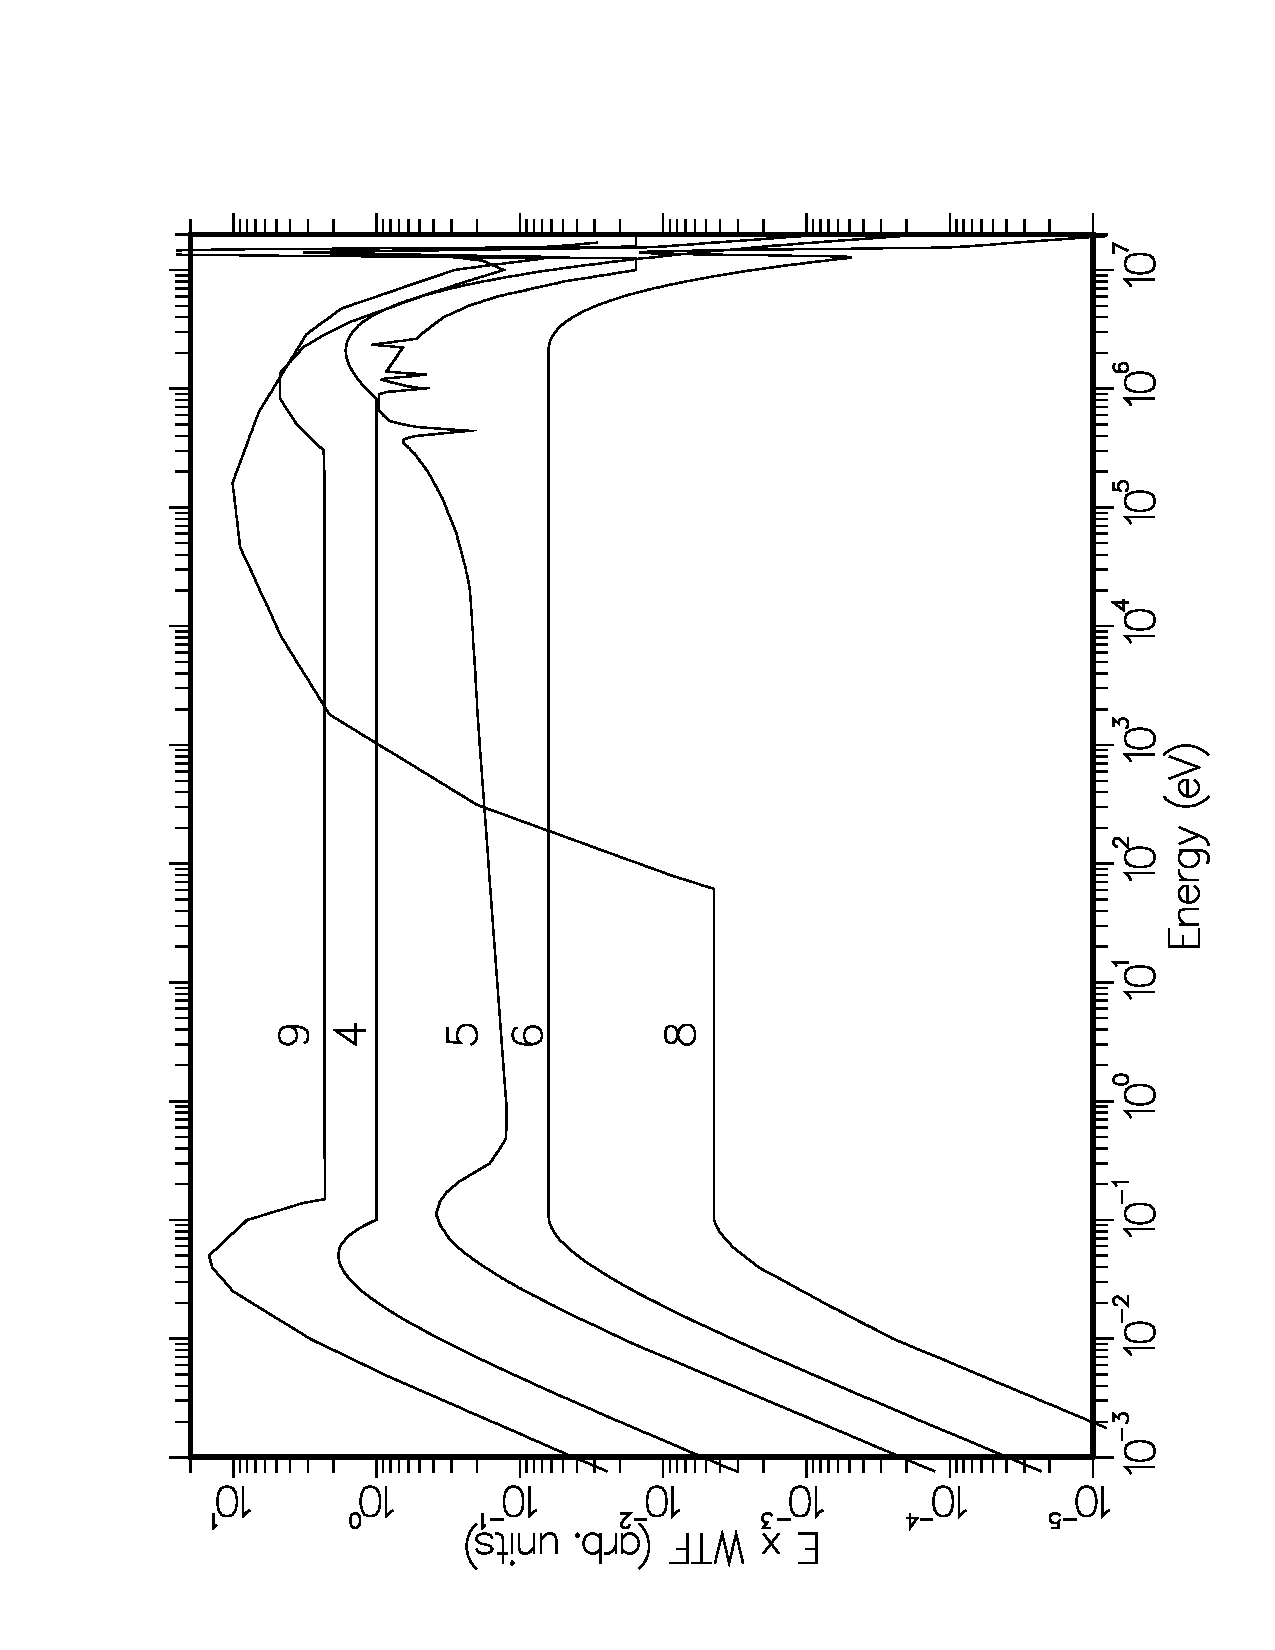
\includegraphics[keepaspectratio, height=3.9in, angle=270]{figs/appb1ack}
\caption[GROUPR weight functions on a logarithmic flux/unit lethargy
 scale]{Built-in neutron weight functions of GROUPR on a logarithmic
 flux-per-unit-lethargy plot that emphasizes the low energy range.}
\label{fig-leth}
\end{figure}

The available weight function options are listed in the input
instructions under \cword{iwt}.  See Fig.~\ref{fig-leth} and
Fig.~\ref{fig-lin}.  Here are brief descriptions of the options:

\begin{figure}[t]\centering
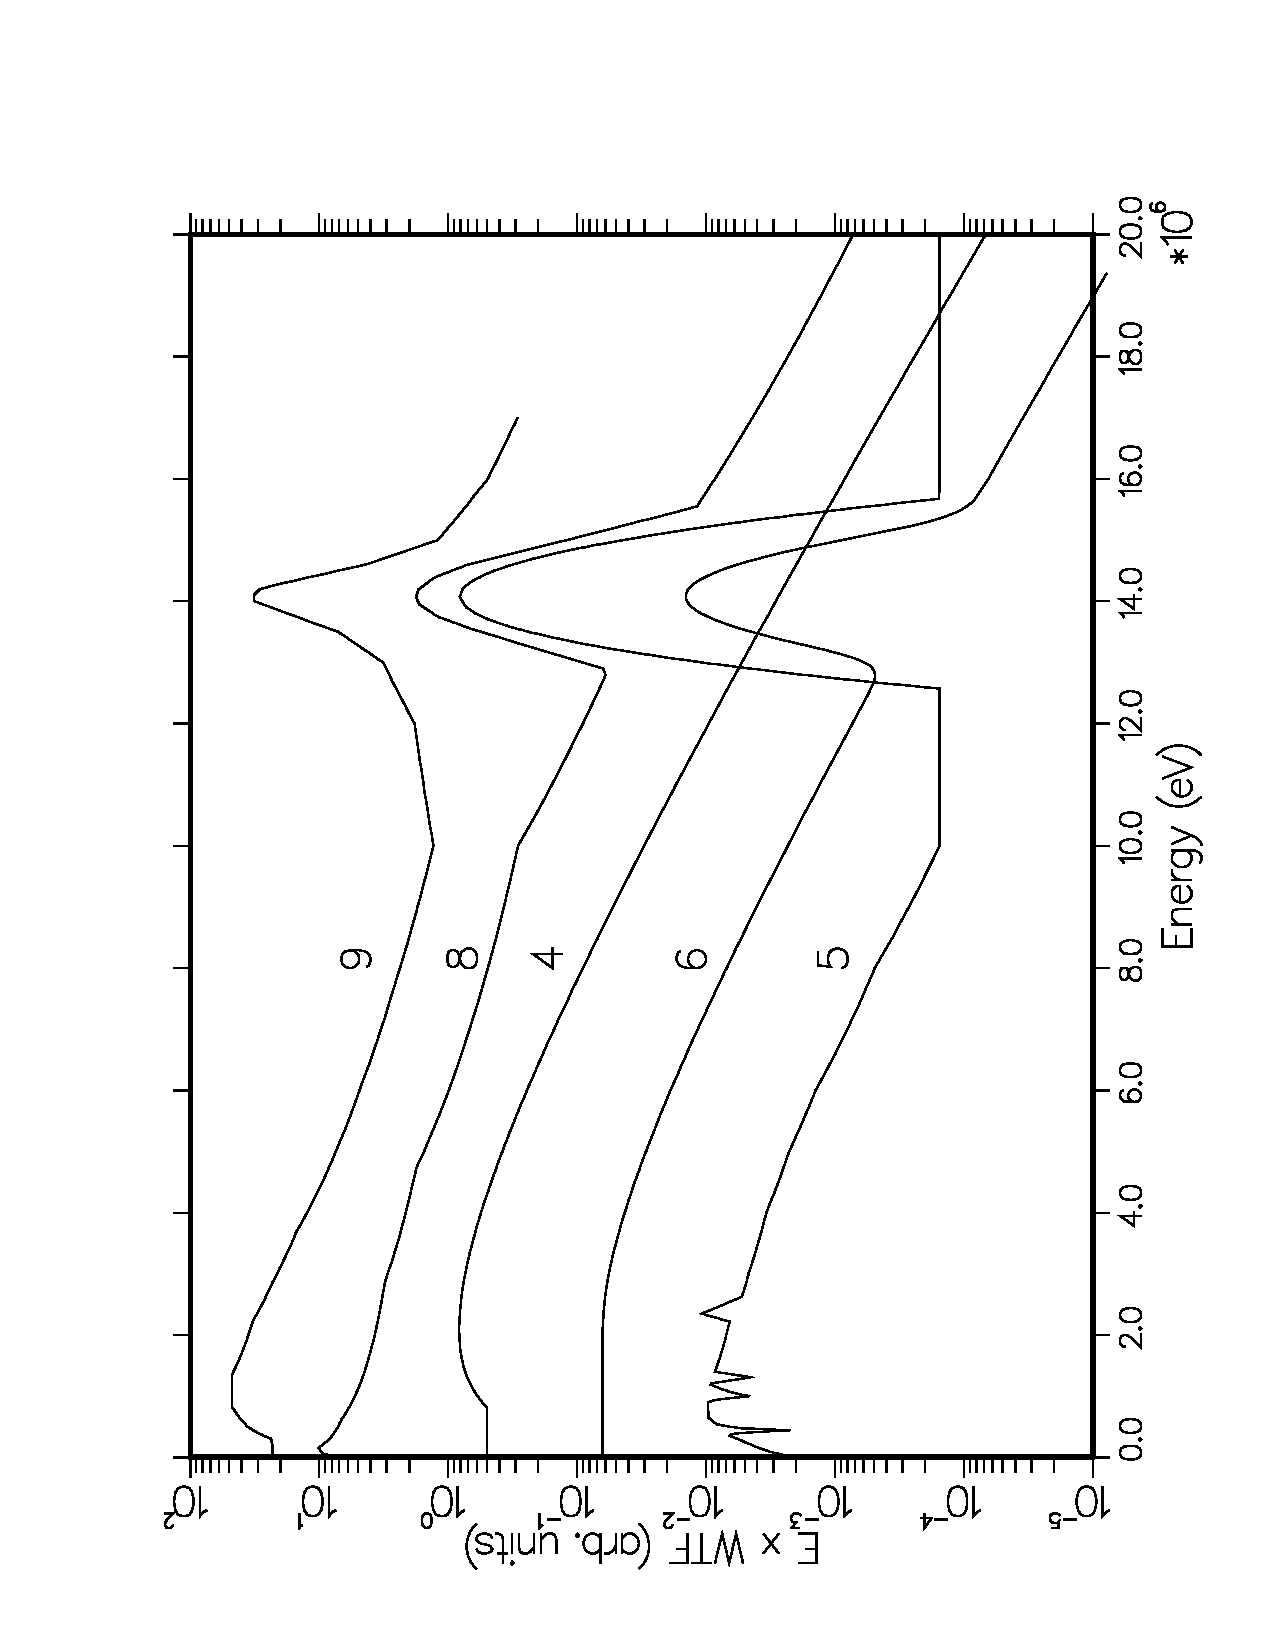
\includegraphics[keepaspectratio, height=3.9in, angle=270]{figs/appb2ack}
\caption[GROUPR weight functions on a linear energy scale]{Built-in neutron
 weight functions on a linear plot that emphasizes the high-energy range.}
\label{fig-lin}
\end{figure}

\begin{description}
\begin{singlespace}
\item{IWT=2\ } The weight function is constant (not shown in the Figures).
   This option is usually chosen for very fine group
   structures such as the 620-group or 640-group
   dosimetry structures.

\item{IWT=3\ } The weight function is proportional to $1/E$.
   The slowing-down of neutrons in water gives a $1/E$
   flux from about 1 eV up to 100 keV, or so.  This
   weight function is traditionally used for
   calculating resonance integrals, but it is not
   useful at the lower and higher energies needed for a
   full set of transport constants.  Although not shown, the graph
   of this function is a flat line on a flux-per-unit-lethargy
   plot, such as the one in Fig.~\ref{fig-leth}.

\item{IWT=4\ } This weight function combines a thermal Maxwellian at low
   energies, a $1/E$ function at intermediate energies, and a
   fission spectrum at high energies to obtain a function appropriate
   for several different applications.  The temperatures of the
   Maxwellian and fission parts and the energies where the components
   join can be chosen by the user.  Therefore, option 4 can be used
   to produce typical thermal reactor weight functions like those
   shown in Figures~\ref{fig-leth} and \ref{fig-lin}, a pure fission
   spectrum for calculating some kinds of dosimetry cross sections, or a
   pure thermal spectrum for getting effective thermal average cross
   sections.  The function  for IWT=4 shown in the figure was produced
   using a thermal temperature of 0.025 eV joined to $1/E$ at 0.1~eV,
   and a fission temperature of 1.40 MeV joined to $1/E$ at 820.3 keV.

\item{IWT=5\ } This is a mid-life PWR (pressurized water reactor) flux
   spectrum with a fusion peak added (see below for a discussion of the
   fusion peak used).  Note the peaks and dips resulting from oxygen
   resonances and windows at high energies, and the hardening apparent
   in the epithermal region.  The thermal part of the function is also
   hardened with respect to a simple Maxwellian shape.  The dips that
   should show up in the eV range due to resonances and $^{238}$U have been
   removed to allow the self-shielding method to work without risk of
   counting the shielding effects twice.  This weight function has
   been used for several libraries\cite{powr} prepared for the Electric
   Power Research Institute (EPRI)\index{EPRI}, and for the MATXS7 library
   used with the TRANSX code\index{TRANSX}.

\item{IWT=6\ } This function is similar to option 4, but the breakpoints
   were chosen to keep the curves continuous.  The thermal Maxwellian
   is calculated for 300K.  In this case, the fusion peak (see below)
   was added to the high-energy tail of the fission spectrum for
   smoothness.

\item{IWT=7\ }  This option is reserved for future use.

\item{IWT=8\ } This function is intended for cross sections libraries
   used for fast reactor analysis (typically, fast breeder
   designs), but is also useful for fusion-blanket problems.  It has
   a fusion peak at high energies, followed by a fission spectrum, a
   slowing-down spectrum typical of a fast reactor, and a thermal tail.
   The tail is provided to help give reasonable results in shields
   far from the core; its characteristic temperature is 300K.  Note
   the sharp drop in the flux as energy decreases from 19 keV.  This
   region is important for $^{238}$U absorption, and this drop-off helps
   to give good group constants for fast reactors.  Of course, it
   would be entirely wrong for a thermal reactor.

\item{IWT=9\ } This is another typical thermal+$1/E$+fission+fusion
   function that has been used for many libraries at LANL
   in the 30-group structure.  The CLAW-3 and
   CLAW-4 libraries are available from the Radiation Shielding
   Information Computational Center at ORNL.

\item{IWT=10\ } This is the same as the CLAW weight function
   (IWT=9), but the shape of the thermal part is automatically
   recalculated to follow a Maxwellian law for temperature $T$.

\item{IWT=11\ } This is the weight function used in the
   VITAMIN-E library.  It has the following segments:
   a .0253-eV thermal Maxwellian below 0.414 eV, a $1/E$ law from
   .414 eV to 2.12 MeV, a 1.415-MeV fission spectrum from 2.12 to
   10 MeV, another $1/E$ section from 10 to 12.52 MeV, a fusion
   peak (25 keV width) between 12.52 and 15.68 MeV, and a final
   $1/E$ section for all higher energies.  The shape of the fusion
   peak is almost identical to IWT=5 (see Fig.~\ref{fig-lin}).  The
   low-energy part of this weight function is not shown.
\end{singlespace}
\end{description}

\noindent
Just as in the case of group structures, an arbitrary weight
function can be read in (see \cword{card8b}).  This function is
presented to GROUPR as an ENDF/B ``TAB1'' record.  This means that a
count of $E,C(E)$ pairs and one or more interpolation schemes are given.

An ENDF/B ``TAB1'' record consists of three distinct parts:
\begin{itemize}
\item two double values and four integer values of which only the last
two integers (the number of interpolation ranges \cword{NR} and the number
of $E,C(E)$ pairs \cword{NP}) are needed to read the remainder of the record
\item the interpolation scheme data which is a sequence of \cword{NR} pairs
of \cword{NBT} (index of the $E,C(E)$ pair corresponding to the end of
interpolation range) and \cword{INT} (the interpolation type)
\item the tabulated data which is a sequence of \cword{NP} $E,C(E)$ pairs
\end{itemize}

\noindent
The interpolation type \cword{INT} specifies the interpolation law to be used in the
interpolation range. It can take the following values:

\begin{center}
\begin{tabular}{cl}
\cword{INT} & Meaning \\ \hline
1 & histogram\\
2 & linear-linear\\
3 & linear-log\\
4 & log-linear\\
5 & log-log \\ \hline
\end{tabular}
\end{center}

\noindent
For example, \cword{INT}=5 specifies that ln$C$ is a linear function of ln$E$.
Similarly, INT=4 specifies that ln$C$ is a linear function of $E$.

\noindent
In its most general form, these input cards would be

\small
\begin{ccode}

   0.      0.      0       0       NR      NP
   NBT(1)  INT(1)    ...   NBT(NR) INT(NR)
   E(1)    C(1)      ...   E(NP)   C(NP)        / card8b

\end{ccode}
\normalsize

\noindent
For example, a function using two interpolation ranges: the first one
between 1e-5 eV and 100 eV using a histogram and the second one between
100 eV and 20 MeV using lin-lin interpolation)

\small
\begin{ccode}

   0.      0.      0       0       2       6
   3       1       6       2
   1e-5    0.5     1.      0.75    100.    0.8
   1e+6    0.85    1.5e+6  0.9     2.0e+7  1.0  / card8b

\end{ccode}
\normalsize

\noindent
For the special case of a single interpolation scheme, the input cards
are simplified as follows

\small
\begin{ccode}

   0.      0.      0       0       1       NP
   NP      INT
   E(1)    C(1)      ...   E(NP)   C(NP)        / card8b

\end{ccode}
\normalsize

\noindent
As many physical lines as are needed can be used for ``\cword{card8b}'',
as long as the terminating slash is included.

One of the weighting options, IWT=4, is a generalized
``$1/E$+fission+thermal'' function where the thermal temperature,
fission temperature, and breakpoint energies (all in eV) are given
on \cword{card8c}.  The weight function for the Los Alamos LIB-IV
cross section library\cite{LIBIV} used
\index{LIB-IV}

\small
\begin{ccode}

   .10 .025 820.3e3 1.4e6 / card8c

\end{ccode}
\normalsize

\noindent
See Figures~\ref{fig-leth} and \ref{fig-lin} for a plot of this function.

Several of these weight functions include a fusion peak\index{fusion peak}.
Because of the finite width of the distribution of ion
energies in a D-T fusion plasma, the emitted 14-MeV
neutrons clearly will not have a delta-function energy
spectrum.  In fact, owing to the presence of a cross-product
term in the kinematic relations, the typical ion-energy
spread of a few tens of kilovolts is magnified into a
neutron-energy spread of around 1 MeV.
For an assumed isotropic Maxwellian plasma, the neutron peak
shape (for example, see the review article by Lehner\cite{one}) is

\begin{equation}
  S(E)=C\int_0^\infty \exp\{-b\bigl[v^2+v_0(g)^2\bigr]-cg^2\}
  \sinh(2bvv_0)\,{{g^3\sigma(g)}\over{v_0(g)}}\,dg \,\,.
\label{lehner}
\end{equation}

\noindent
Here $S(E)$ is the number of neutrons emitted with laboratory
energy between $E$ and $E+dE$, $C$ is a normalization
factor, $v$ is the laboratory velocity corresponding to
energy $E$, and $v_0$ is the velocity of the neutron in
the CM system.  Both $v_0$ and the fusion cross section
$\sigma$ are determined by the relative velocity $g$ of
the reacting ions, the integration variable in Eq.~\ref{lehner}.
The coefficient $b$ is equal to $M/2kT$, where $M$ is the
total mass of the reacting ions and $kT$ is the plasma
temperature.  Similarly, $c$ is $\mu /2kT$, where $\mu$
is the reduced mass of the ion system.
The only approximation involved in Lehner's derivation
of Eq.~\ref{lehner} is that all particles may be treated
nonrelativistically.  At 14 MeV, the relativistic factor

\begin{equation}
  \gamma={{1}\over{\sqrt{1-v^2/c^2}}}\,\,,
\end{equation}

\noindent
is very close to unity (1.015), and it varies negligibly over
the range of interest (say, 13 to 17 MeV).  It is sufficient
then to invoke relativistic mechanics in defining the location
of the 14-MeV peak but not in discussing the shape.  This
effect  moves the peak toward lower neutron energies, but
only by about 20 keV.  Although the expression for $S(E)$
in Eq.~\ref{lehner} is accurate, it has the disadvantage of
requiring a numerical integration at each point $E$ in the
energy spectrum.  For this reason, we consider what
simplifications can be made without serious loss
of accuracy.  In the energy range around the 14-MeV peak, the
product $2bvv_0$ in Eq.~\ref{lehner} has a numerical value of
about 6000.  Thus, the hyperbolic sine can obviously be replaced
by just the positive exponential term.  If we make this change in
Eq.~\ref{lehner}, we can write the following, still nearly exact,
expression for the neutron spectrum:

\begin{equation}
  S_1(E)=C_1 \int_0^\infty \exp[-b(v-v_0)^2]\,P(v_0)\,dv_0 \,\,.
\label{intexp}
\end{equation}

\noindent
Here we also have inverted the function $v_0(g)$ and changed the
integration variable.  The spectrum then is a linear superposition
of velocity exponentials with slightly different peak locations.
For normal plasma temperatures, the velocity distribution
$P(v_0)$ is very narrow, since the expression for $v_0$ is
dominated by the nuclear Q-value (17.586 MeV) rather than the
contribution from the ion kinetic energy (typically around
50 keV).  Thus, it seems reasonable to approximate $P(v_0)$ as
delta function

\begin{equation}
  P(v_0) \approx \delta(v_0-v_p) \,\,.
\end{equation}

\noindent
This gives a second approximate form,

\begin{equation}
  S_2(E)=C_2 \exp[-b(v-v_p)^2] \,\,,
\label{velexp}
\end{equation}

\noindent
where $v_p$ has the obvious meaning of the laboratory neutron
velocity at the center of the peak.  We shall refer to this as
the velocity exponential form of the neutron energy spectrum.
An expression essentially identical to Eq.~\ref{velexp} was
given in an early paper by Nagle and coworkers\cite{two}.
In order to examine the accuracy of the velocity exponential form,
we have calculated $S(E)$ from Eq.~\ref{lehner}
and $S_2(E)$ from Eq.~\ref{velexp}
at 20 keV, a typical plasma temperature in current fusion-reactor
concepts.  In performing the numerical integration over $g$ in
Eq.~\ref{lehner}, we used numerical values for the D-T fusion cross
section taken from the compilation by Jarmie and Seagrave\cite{three}.
In evaluating $S_2(E)$ using Eq.~\ref{velexp}, a value of $v_p$ was
chosen so as to force agreement between $S_2(E)$ and $S(E)$ at
17 MeV.  As discussed by Muir\cite{four}\index{Muir}, the overall
agreement is remarkably good, the maximum error
over the range from 13.5 to 17 MeV being about 2\%.  The value of
$v_p$ thus derived corresponds to a peak-center energy $E_p$
of 14.07 MeV.  This value includes the small ($\sim$ 20 keV)
relativistic correction mentioned above.  If we approximate the
mass of the D{+}T system as 5 times the neutron mass, then we
obtain the recommended peak shape

\begin{equation}
  S_{\rm rec}(E)=\exp \bigl[ -{5 \over{kT}}(\sqrt{E}
  -\sqrt{E_p})^2 \bigr] \,\,,
\label{muir}
\end{equation}

\noindent
where $E_p{=}14.07\,{\rm MeV}$.  The functional form in Eq.~\ref{muir}
was used to calculate the fusion peak shapes appearing in two
of the data statements in \cword{genwtf}\index{genwtf@{\ty genwtf}}
(namely, those utilized for IWT=5 and 8) and  is also  used explicitly
in \cword{getwtf}\index{getwtf@{\ty getwtf}} to calculate analytically
the weight function for IWT=6.  In all three cases, $kT$=25 keV is
used as an average or typical fusion-reactor plasma temperature.
See Fig.~\ref{fig-lin} for a graphical display of the resulting
weight functions in the 14-MeV region.

The GROUPR flux calculator\index{flux calculator} is selected by
a negative sign on \cword{iwt}.  The additional \cword{card8a} is
then read.  The calculator option used is determined by the number
of parameters given and their values.  The parameters \cword{fehi}
and \cword{nflmax} are used to select the energy range for the
flux calculation, and they also determine the cost in time
and storage.  The actual value for \cword{sigpot} is not very
critical -- a number near 10 barns is typical for fissionable materials.

Nonzero values for \cword{ninwt} and \cword{jsigz} will cause the
computed flux for a given fissionable isotope (such as $^{238}$U) to be
written out onto a file.  This saved flux can be used as input for a
subsequent run for a fissile material (such as $^{239}$Pu) with
\cword{iwt}=0 to get an approximate correction for resonance-resonance
interference.  See Eq.~\ref{Eq38}.

Nonzero values for some of the last five parameters on \cword{card8a}
select the extended flux calculation of Eq.~\ref{Eq37}.  The simplest
such calculation is for an isolated pin containing a heavy absorber
with an admixed moderator.  For $^{238}$UO$_2$, the card might be

\small
\begin{ccode}

   400 10.6 5000 0 0 .7768 7.5 / card8a

\end{ccode}
\normalsize

\noindent
where 7.5 barns is twice the oxygen cross section and $\alpha$ is computed
from $\bigl[ (A-1)/(A+1)\bigr] ^2$ with $A=15.858$.  A more general case
would be a PWR-like lattice of $^{238}$UO$_2$ fuel rods in water:

\small
\begin{ccode}

   400 10.6 5000 0 0 .7768 7.5 .40 1.7e-7 0.086 / card8a

\end{ccode}
\normalsize

\noindent
where 0.086 is computed using 3.75 barns for O and 40 barns for the
two H atoms bound in water; that is,

\begin{equation}
  \gamma = \frac{3.75}{2*20 + 3.75}  = 0.086\;.
\end{equation}
\vspace{0.5 pt}

\noindent
A third example would compute the flux for a homogeneous mixture of
$^{238}$U and hydrogen

\small
\begin{ccode}

   400 10.6 5000 0 0 0 0 1. 1.7e-7 / card8a

\end{ccode}
\normalsize

\noindent
As a final example, consider a homogeneous mixture of uranium and water.
This requires \cword{beta}=1 and \cword{sam}=0.  Thus,

\small
\begin{ccode}

   400 10.6 5000 0 0 .7768 0. 1. 1.7e-7 .086 / card8a

\end{ccode}
\normalsize

The maximum Legendre expansion order used for scattering matrices is set
by \cword{lord}.  The number of tables produced is \cword{lord}+1; that is,
$\ell=0$, 1, ... \cword{lord}.  When more than 1 value of $\sigma_0$
is requested, both the $\ell{=}0$ and $\ell{=}1$ components of the
total cross section are produced.

Card 3 contains a short descriptive title that is printed on the listing
and added to the output GENDF tape.  Card 4 gives the \cword{ntemp} values
of temperature for the run.  They must be in ascending order, and if
unresolved data are included on the PENDF tape, the temperatures in this
list must match the first \cword{ntemp} values in MF=2, MT=152 from
\hyperlink{sUNRESRhy}{UNRESR}\index{UNRESR} or
\hyperlink{sPURRhy}{PURR}\index{PURR} (see
\cword{stounr}\index{stounr@{\ty stounr}} and
\cword{getunr}\index{getunr@{\ty getunr}}).  Card 5 gives the
$\sigma_0$ values for the run in descending order, starting with
infinity (represented by $10^{10}$ barns).

This completes the description of the global input parameters for GROUPR.
The rest of the input cards request reactions to be processed for the
various temperatures and materials desired.  Because of the many types
of data that it can process, GROUPR does not have a completely
automatic mode for choosing reactions to be processed.  On the basic
level, it asks the user to request each separate cross section or
group-to-group matrix using the parameters \cword{mfd}, \cword{mtd},
and \cword{mtname}.  However, simplified input modes are also available.
For example, the one ``\cword{card9}'' containing

\small
\begin{ccode}

    3/

\end{ccode}
\normalsize

\noindent
will process the cross section ``vectors'' for all of the reaction MT
numbers found on the PENDF tape.

For completeness, the full input for \cword{matd}, \cword{mfd},
and \cword{mtname} will be described first.  Most readers can skip
to the description of automated processing below.  The value of
\cword{mfd} depends on the output desired (vector, matrix) and the
form of the data on the ENDF evaluation.  Simple cross section ``vectors''
$\sigma_{xg}$ are requested using \cword{mfd}=3 and the \cword{mtd}
numbers desired from the list of reactions available in the evaluation
(check the directory in MF=1,MT=451 of the ENDF and PENDF tapes for the
reactions available).  A typical example would be

\small
\begin{ccode}

   3   1 'total'/
   3   2 'elastic'/
   3  16 '(n,2n)'/
   3  51 '(n,nprime)first'/
   3 -66 '(n,nprime)next'/
   3  91 '(n,nprime)continuum'/
   3 102 'radiative capture'/

\end{ccode}
\normalsize

\noindent
The combinations of ``3 51'' followed by ``3 $-$66'' means process all
the reactions from 51 through 66; that is, (n,n$'_1$), (n,n$'_2$),
\ldots, (n,n$'_{16}$).  If self-shielding is requested, the following
reactions will be processed using \cword{nsigz} values of background
cross section: total (MT=1), elastic (MT=2), fission (MT=18 and 19),
radiative capture (MT=102), heat production (MT=301), kinematic KERMA
(MT=443), and damage energy production (MT=444).  The other File-3
reactions will be computed at $\sigma_0{=}\infty$ only.  This list of
reactions can be altered by small changes in \cword{init} if desired.

There are several special options for \cword{mtd} available when processing
cross section vectors:

\begin{list}{ }{\labelsep=.25in\leftmargin=1in\labelwidth=.75in}
\begin{singlespace}
\item[\underbar{\cword{mtd}}] \underbar{Option}
\item[259] Average inverse neutron velocity for group in s/m.
\item[258] Average lethargy for group.
\item[251] Average elastic scattering cosine $\overline\mu$
               computed from File 4.
\item[252] Continuous-slowing-down parameter $\overline\xi$
               (average logarithmic energy decrement for elastic
               scattering) computed from File 4.
\item[253] Continuous-slowing-down parameter $\overline\gamma$
               (the average of the square of the logarithmic energy
               decrement for elastic scattering, divided by twice the
               average logarithmic energy decrement for elastic
               scattering) computed from File 4.
\item[452] $\overline\nu$: the average total fission yield
               computed from MF=1 and MF=3.
\item[455] $\overline\nu^D$: the average delayed neutron yield
               computed from MF=1 and MF=3.
\item[456] $\overline\nu^P$: the average prompt fission neutron
               yield computed from MF=1 and MF=3.
\end{singlespace}
\end{list}

\noindent
There are also some special options for \cword{mfd} that can
be used when processing cross sections:

\begin{list}{ }{\labelsep=.25in\leftmargin=1in\labelwidth=.75in}
\begin{singlespace}

\item[\underbar{\cword{mfd}}] \underbar{Option}
\item[12] Photon production cross section computed from File 12 and File 3.
\item[13] Photon production cross section computed from File 13.
          Recent versions of GROUPR will automatically shift
          between 12 and 13, if necessary.
\item[1zzzaaam] nuclide production for zzzaaam from a subsection of MF=3
\item[2zzzaaam] nuclide production for zzzaaam from a subsection of MF=6
\item[3zzzaaam] nuclide production for zzzaaam from a subsection of MF=9
\item[4zzzaaam] nuclide production for zzzaaam from a subsection of MF=10
\item[40000000] fission product production from the MT=18 subsection of MF=10
\end{singlespace}
\end{list}

\noindent
An example of the isomer production capability would be the
radiative capture reaction of ENDF/B-V $^{109}$Ag(n,$\gamma$)
from Tape 532:

\small
\begin{ccode}

   30471090 102 '(n,g) TO g.s.'/
   30471091 102 '(n,n) to isomer'/

\end{ccode}
\normalsize

\noindent
Starting with ENDF/B-VIII.0, some non-fissile nuclides can have an MT=18 section (fission)
in MF=10 (radioactive isotope production) to represent breakup due to high energy
particles. In these cases, it is often not possible to designate a specific nuclide,
which is why the \cword{mfd} value is set to \cword{40000000}. In such a case, the
following input will make GROUPR process this part of the ENDF file:

\small
\begin{ccode}

   40000000  18 'HE breakup' /

\end{ccode}
\normalsize

The next class of reactions usually processed is the group-to-group
neutron scattering matrices.  The complete list of \cword{mtd} values is
most easily found under File 4 in the MF=1,MT=451 ``dictionary''
section of the evaluation.  An example follows:

\small
\begin{ccode}

   6   2 'elastic matrix'/
   6  16 '(n,2n) matrix'/
   6  51 '(n,nprime)first matrix'/
   6 -66 '(n,nprime)next matrix'/
   6  91 '(n,nprime)continuum matrix'/  .

\end{ccode}
\normalsize

\noindent
Using \cword{mfd}=6 implies that File 4, or File 4 and File 5, will
be used to generate the group-to-group matrix.  The elastic matrix will
be computed for \cword{nsigz} values of background cross section, but
the other reactions will be computed for $\sigma_0{=}\infty$ only.  The
list of matrices to be self-shielded can be altered by changing
\cword{init}.

Fission is more complex.  For the minor isotopes, only
the total fission reaction is used, and the following input is appropriate
for the prompt component:

\small
\begin{ccode}

   3 18 'fission xsec'/
   6 18 'prompt fission matrix'/

\end{ccode}
\normalsize

\noindent
For the important isotopes, partial fission reactions are given.  They
are really not needed for most fission reactor problems, and the input
above is adequate.  However, for problems where high-energy neutrons
are important, the following input should be used:

\small
\begin{ccode}

   3 18 'total fission'/
   3 19 '(n,f)'/
   3 20 '(n,nf)'/
   3 21 '(n,2nf)'/
   3 38 '(n,3nf)'/
   6 19 '(n,f)'/
   6 20 '(n,nf)'/
   6 21 '(n,2nf)'/
   6 38 '(n,3nf)'/

\end{ccode}
\normalsize

\noindent
Note that ``6 18'' is omitted because it will, in general, be different
from the sum of the partial matrices (see Section~\ref{ssGROUPR_FissSource}).
Some materials don't have data for (n,3nf); in these cases, omit the two
lines with \cword{mtd}=38 from the input.  The fission matrix is not
self-shielded.  Since resonance-to-resonance fission-spectrum variations
are not described in the ENDF format, it is sufficient to self-shield
the cross section and then to use the self-shielding factor for the
cross section to self-shield the fission neutron production.

Delayed fission data are available for the important actinide isotopes,
and the following input to GROUPR is used to process them:

\small
\begin{ccode}

   3 455 'delayed nubar'/
   5 455 'delayed spectra'/

\end{ccode}
\normalsize

\noindent
The line for \cword{mfd}=5 automatically requests spectra for all time groups
of delayed neutrons.  The time constants are also extracted from
the evaluation.  As discussed in Section~\ref{ssGROUPR_FissSource},
formatting modules such as \hyperlink{sDTFRhy}{DTFR} and
\hyperlink{sCCCCRhy}{CCCCR} must combine the prompt and delayed
fission data written onto the GENDF tape in order to obtain steady-state
fission parameters for use in transport codes.

Starting with the ENDF-6 format, neutron production data may also be
found in File 6, and \cword{mfd}=8 is used to tell the code
to use MF6 for this \cword{mtd}.  When using full input, the user
will have to check the File 1 directory and determine what subsections
occur in File 6.

Photon production reactions can be found in the ENDF dictionary under
MF=12 and 13.  To request a neutron-to-photon matrix, add 4 to this
number.\footnote{In recent versions of NJOY, GROUPR will automatically
shift between 16 and 17 using data read from the ENDF dictionary by
the \cword{conver} subroutine.  Thus, use of \cword{mfd}=17 is no longer
necessary.}  For example,

\small
\begin{ccode}

   17   3 'nonelastic photons'/
   16   4 'inelastic photons'/
   16  18 'fission photons'/
   16 102 'capture photons'/

\end{ccode}
\normalsize

\noindent
Yields (MF=12) are normally used with resonance reactions (MT=18 or MT=102),
or for low-lying inelastic levels (MT=51, 52, ....).  MT=3 is often used
by evaluators as a catch-all reaction at high energies where it is
difficult to separate the source reactions in total photon emission
measurements.  In these cases, photon production cross sections from
other reactions like MT=102 are normally set equal to zero at high
energies.  The general rule for photon emission is that the total
production is equal to the sum of all the partial production reactions
given in the evaluation.   Starting with the ENDF-6 format, photon
production may also appear in File 6.  Use \cword{mfd=18} to process
these contributions.  Since resonance-to-resonance variations in
photon spectra are not given in ENDF evaluations, GROUPR does not normally
self-shield the photon production matrices (although this can be done
if desired by making a small change in \cword{init}); instead, it is
assumed that only the corresponding cross section needs to be shielded.
Subsequent codes can use the cross section self-shielding factor with the
infinite-dilution photon production matrix to obtain self-shielded photon
production numbers.

This version of GROUPR can also generate group-to-group matrices for
charged-particle production from neutron reactions and for all kinds
of matrices for incident charged particles.  The incident particle is
determined by the input tape mounted.  The identity of the secondary
particle is chosen by using one of the following special \cword{mfd}
values:

\begin{center}
For distributions given in File 6 (energy-angle):
\vspace{6 pt}
\begin{tabular}{cl}
  \cword{  mfd  } & Meaning \\ \hline
           21     &  proton production \\
           22     &  deuteron production \\
           23     &  triton production \\
           24     &  $^{3}$He production \\
           25     &  alpha production \\
           26     &  residual nucleus (A$>$4) production \\ \hline
\end{tabular}
\end{center}

\vspace{4 pt}

\begin{center}
For distributions given in File 4 (angle only):
\vspace{6 pt}
\begin{tabular}{cl}
  \cword{  mfd  } & Meaning \\ \hline
           31     &  proton production \\
           32     &  deuteron production \\
           33     &  triton production \\
           34     &  $^{3}$He production \\
           35     &  alpha production \\
           36     &  residual nucleus (A$>$4) production \\ \hline
\end{tabular}
\end{center}
\vspace{4 pt}

\noindent
If necessary, \cword{mfd}=21-26 will automatically change to 31-36.

The user will normally process all reactions of interest at the first
temperature (for example, 300K).  At higher temperatures, the threshold
reactions should be omitted, because their cross sections do not change
significantly with temperature except at the most extreme conditions.
This means that only the following reactions should be included for
the higher temperatures (if present): total (MT=1), elastic (MT=2),
fission (MT=18), radiative capture (MT=102), heating (MT=301),
kinematic KERMA (MT=443)\index{KERMA}, damage (MT=444)\index{damage},
and any thermal cross sections (MT=221-250).  Only the elastic and
thermal matrices should be included at the higher temperatures.

\underbar{Warning}: when using the explicit-input option, it is a fatal
error to request a reaction that does not appear in the evaluation,
cannot be computed from the evaluation, or was not added to the
PENDF tape by a previous module.  Reactions with thresholds above
the upper boundary of the highest energy group will be skipped after
printing a message on the output file.

Automated processing of essentially all reactions included in an ENDF/B
evaluation is also available.  As mentioned previously, the single card

\small
\begin{ccode}

   3/

\end{ccode}
\normalsize

\noindent
will process all the reactions found in File 3 of the input PENDF tape.
However, this list excludes thermal data (MT=221-250) and special
options such as \cword{mtd}=251-253, 258-259, and 452-456.  If any of these
reactions are needed, they should be given explicitly (see example below).
Similarly, the single card

\small
\begin{ccode}

   6/

\end{ccode}
\normalsize


\noindent
will process the group-to-group matrices for all reactions appearing in
File 4 of the ENDF/B tape, except for MT=103-107 and thermal scattering
matrices (MT=221-250).  If MT=18 and 19 are both present, only MT=19
will be processed into a fission matrix.  For ENDF-6 evaluations, the
``\cword{8/}'' option will also process every neutron-producing subsection in
File 6.  Photon production cross sections are requested using

\small
\begin{ccode}

   13/

\end{ccode}
\normalsize

\noindent
and photon-production matrices are requested with the single card

\small
\begin{ccode}

   16/

\end{ccode}
\normalsize

\noindent
In both cases, all reactions in both File 12 and File 13 will be processed
without the need for using \cword{mfd}=12 or \cword{mfd}=17.  For ENDF-6
libraries, this option will also process all photon-production subsections
in File 6.  There is no automatic option for delayed neutron data.  An
example of a processing run for a fissionable isotope with thermal
cross sections follows:

\small
\begin{ccode}

   3/
   3 221/ thermal xsec
   3 229/ average inverse velocity
   3 455/ delayed nubar
   5 455/ delayed spectra
   6/
   6 221/ thermal matrix
   16/ photon production matrix

\end{ccode}
\normalsize

\noindent
An example of charged-particle processing for the incident-neutron
part of a coupled n-p-$\gamma$ library follows:

\small
\begin{ccode}

   3/ cross sections
   6/ neutron production matrix
   16/ photon production matrix
   21/ proton production matrix

\end{ccode}
\normalsize

\noindent
The layout of data in a n-p-$\gamma$ coupled set is shown in
Figure~\ref{npg}.

\begin{figure}[thb]\centering
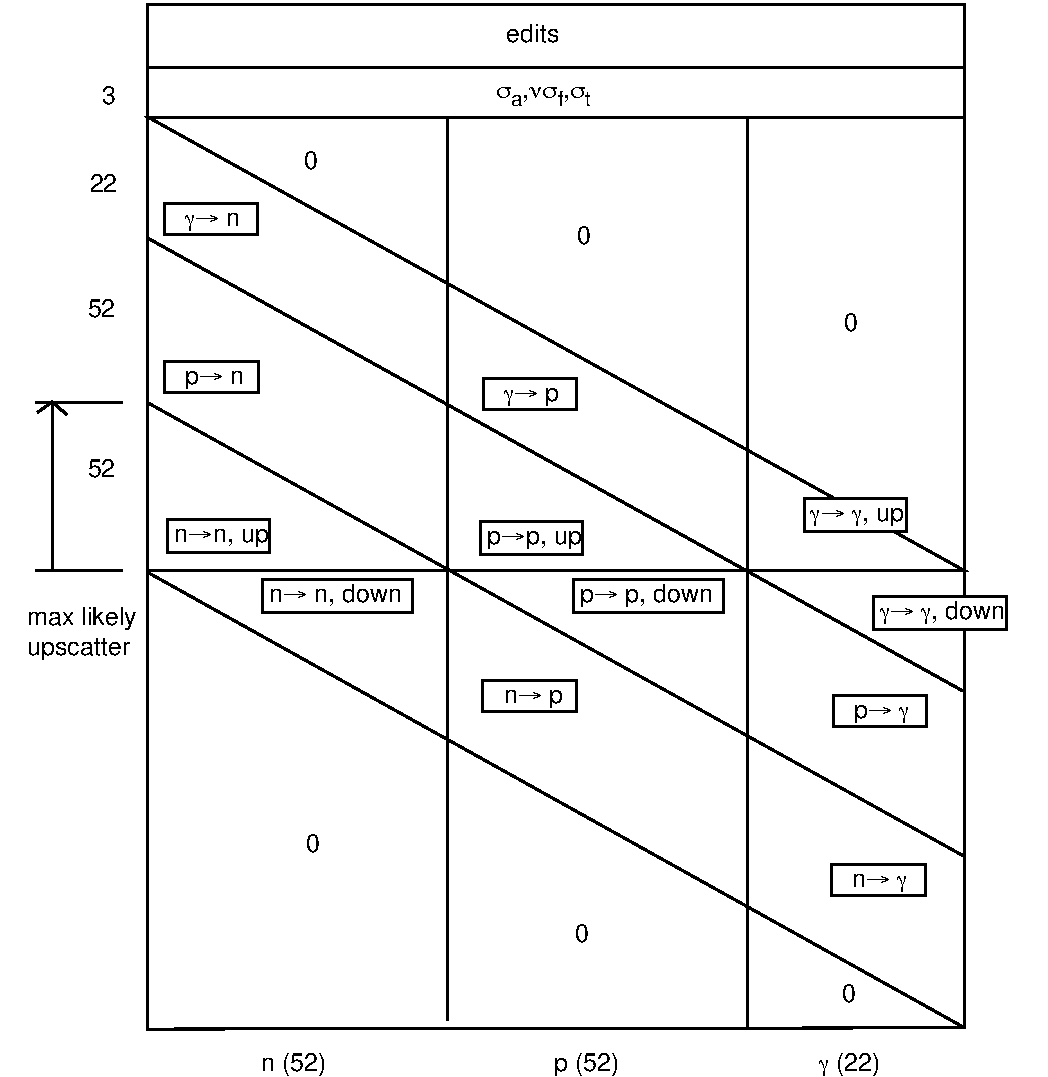
\includegraphics[keepaspectratio, height=5.5in, angle=0]{figs/groupr8}
\caption[Coupled neutron-proton-photon table]{Layout of a coupled table for
 the simultaneous transport of neutrons, protons, and gamma rays.  Normally,
 only the lower triangle of the ``p to n'' block would contain values for the
 upscatter portion of the table (the part above the line in the middle).  The
 ``group'' index increases from left to right, and the ``position'' index
 increases from top to bottom.}
\label{npg}
\end{figure}

There is a new ENDF format now becoming available that helps to
describe the production of all isotopes and isomers in a given system.
It uses a directory in File 8 to direct the code to productions
represented by MF=3, by MF=9 times MF=3, by MF=10, or by sections
of MF=6 times MF=3.  When this format is used, it is possible to
give the simple command

\small
\begin{ccode}

 10/

\end{ccode}
\normalsize

\noindent
to have production cross sections generated for every nuclide that
is produced.  These production sections are labeled with the ZA and
isomeric state of the products for use by subsequent NJOY modules.


\subsection{Coding Details}
\label{ssGROUPR_details}

The \cword{groupr}\index{groupr@{\ty groupr}} subroutine is exported
by the \cword{groupm}\index{modules!groupm@{\ty groupm}} module.
GROUPR begins by reading most of the user's input (see
\cword{ruinb})\index{ruinb@{\ty ruinb}}.  It then
locates the desired material and temperature on the input ENDF,
PENDF\index{PENDF}, and GENDF\index{GENDF} tapes, and reads in
the self-shielded unresolved cross sections (if any) from the PENDF
tape using \cword{stounr}\index{stounr@{\ty stounr}}.  If
self-shielding was requested, \cword{genflx}\index{genflx@{\ty genflx}}
is used to compute the weighting flux as described in
Section~\ref{ssGROUPR_WtFlux}.  The
next step is to write the header record for this material on the
output GENDF tape.

The code is now ready to begin the loop over reactions for this
material and temperature.  Either an input card is read to
get \cword{mfd}, \cword{mtd} and \cword{mtname} (the reaction name),
or the next reaction in
an automatic sequence is selected.  First, the default Legendre order,
secondary group count, and $\sigma_0$ count are selected for the reaction
in \cword{init}\index{init@{\ty init}}, and the retrieval routines are
initialized.  \cword{groupr} then processes the reaction using the
\cword{panel} logic described in
Section~\ref{ssGROUPR_GrpInt}.  If a ``shortcut'' fission
spectrum was requested (\cword{mfd=5}), for delayed fission, and
for the low-energy ``constant'' spectra, the spectrum is calculated
directly using \cword{getff}\index{getff@{\ty getff}}.  As the cross
sections for each group are obtained, they are printed out
(see \cword{displa}\index{displa@{\ty displa}}) and written to the
GENDF tape.  When the last group has been processed, \cword{groupr}
loops back to read a new input card for a new reaction.

This loop over reactions continues until a terminating ``\cword{0/}'' card is
read.  \cword{groupr} then proceeds to the next temperature, if any, and
repeats the loop over reactions.  After the last temperature has been
processed for the first material, an opportunity is provided to change
to a new material, keeping all the other input parameters unchanged.
A ``\cword{0/}'' card at this point causes all the files to be closed, prints
out the final messages, and terminates the \cword{groupr} run.

Automatic choice of the next reaction to be processed is done in one of
two ways.  For a simple range of MT numbers, such as the example 51 - 66
used above, the negative value is stored in the variable \cword{mtdp}
in the \cword{groupr} subroutine.  When \cword{mtdp} is negative,
\cword{mtd} is incremented after each reaction until it is greater than
the absolute value of \cword{mtdp}.  \cword{mtdp} is then reset to one,
and the code proceeds to the next input card.  When processing photon
data, \cword{mfd}=\cword{16}
will automatically change to \cword{17}, if necessary.  Similarly,
\cword{mfd}=21, 22, \ldots will automatically change to
\cword{mfd}=31, 32, \ldots.  A more automatic method is triggered by
\cword{mtd}=0.  In this case, a subroutine called
\cword{nextr}\index{nextr@{\ty nextr}} is called to return
the next value of \cword{mtd} to be used, and a subroutine called
\cword{namer}\index{namer@{\ty namer}} is called to generate the
reaction name.  For \cword{mfd}=3, \cword{nextr} finds the next
reaction in File 3 on the input PENDF tape.  MT=251-253 and
thermal data (MT=221-250) are excluded.  The MT values for the
special options (258, 259, {\it etc.}) do not appear on the PENDF
tape, and they must be requested explicitly.  For matrices,
GROUPR works with a set of lists loaded into global arrays by
\cword{conver}\index{conver@{\ty conver}}.  The list \cword{mf4}
contains all the neutron-scattering MT numbers that appear in the
File 4 part of the directory on the ENDF tape, and the list
\cword{mf6} contains all the MT numbers of sections of File 6 that
contain subsections that produce neutrons.  Therefore, reading
through these two lists returns all the neutron-producing matrix
reactions.  Similarly, the list \cword{mf12} contains all the
File 12 entries from the directory, \cword{mf13} contains the
File 13 entries, and \cword{mf18} contains all the MT
values for sections in File 6 that contain subsections for photon
production.  Scanning through these three lists produces all the
photon production matrix reactions.  Two arrays are used for
charged-particle producing reactions; the first index runs through
the charged particles in the order p, d, t, $^3$He, $\alpha$, recoil.
Taking proton production as an example, the list elements
\cword{mf6p(1,i)} contain the MT numbers of sections in File 6 that
contain subsections that produce protons.  The list elements
\cword{mf4r(1,i)} contain MT numbers from File 4 for two-body reactions
that produce protons; namely, MT600 - MT648.  \cword{nextr} scans through
both of these lists to return indexes to all the reactions that produce
protons.  The same procedure is used for the other charged particles.
The arrays \cword{mf10s} and \cword{mf10i} are used in a similar
way for nuclide production.

Subroutine \cword{namer}\index{namer@{\ty namer}} generates name
strings with up to 15 Hollerith words with 4 characters each
(60 characters).  The names depend on the ``ZA'' of the projectile
and the MT number for the reaction.  The parameter \cword{mfd}
is used to choose between the suffixes ``cross section'' and
``matrix''.   Some examples of the names produced follow:

\begin{center}
\begin{tabular}{lll}
   Name   &   Name   &   Name  \\ \hline
  \cword{(n,total)}   &  \cword{(n,heat)}  &  \cword{(p,p02)}  \\
  \cword{(n,elastic)} &  \cword{(n,p02)}   &  \cword{(p,n00)}  \\
  \cword{(n,2n)}      &  \cword{(p,elastic)}  &  \cword{(g,total)}  \\
  \cword{(n,n01)}     &  \cword{(p,2n)}    &  \cword{(g,pair)}  \\ \hline
\end{tabular}
\end{center}

Subroutines \cword{mfchk}\index{mfchk@{\ty mfchk}} and
\cword{mfchk2}\index{mfchk2@{\ty mfchk2}} are used with the
full input for reaction selection in GROUPR to check whether
\cword{mfd}=17 is needed when \cword{mfd}=16 was requested, or
whether one of the charged-particle File 4 values \cword{mfd}=31-36
is needed when \cword{mfd}=21-26 were requested.  The lists in
global variables like \cword{mf12} are used, just as for \cword{nextr}.

Subroutine \cword{gengpn}\index{gengpn@{\ty gengpn}} generates the
group bounds in the global array \cword{egn} for the neutron group
structure from input cards, from data statements, or by calculation.
Some of the data statements use energies in eV and some use lethargy.
Similarly, \cword{gengpg}\index{gengpg@{\ty gengpg}} generates the
photon group structure in global array \cword{egg} from input cards
or data statements; in this case, all bounds are in eV.

Subroutine \cword{genwtf}\index{genwtf@{\ty genwtf}} sets up the
weight function option requested with \cword{iwt} by reading the
input cards into \cword{weights}, transferring numbers from data
statements to \cword{weights}, or simply reporting the analytic
weight option requested.  Subroutine
\cword{getwtf}\index{getwtf@{\ty getwtf}} returns the values of the
weight function at energy $E$ by calculation or by interpolation
in the table established by \cword{genwtf}.  The current
version returns the same value for all Legendre orders.  Choosing
\cword{enext} is difficult for \cword{getwtf} because the functions have
not been explicitly linearized.  It is important to generate extra grid
points in energy regions where the weight function may vary faster than the
cross section (for example, in the fusion peak).

Subroutine \cword{genflx}\index{genflx@{\ty genflx}} computes the
self-shielded weighting flux using either the Bondarenko model
or the flux calculator, and it writes the result on a scratch tape
using the \cword{loada} utility routine.  When fluxes are needed
for the generalized group integrals, they are read from this
scratch file using \cword{finda}\index{finda@{\ty finda}} (see
\cword{getflx}).  Subroutine \cword{genflx} starts by checking for
the weighting option.  If the Bondarenko model was selected, it
initializes \cword{gety1}\index{gety1@{\ty gety1}} and
\cword{getwtf}\index{getwtf@{\ty getwtf}} to read the total
cross section from the PENDF tape and the smooth weighting function
$C(E)$ set up by \cword{genwtf}\index{genwtf@{\ty genwtf}}.  It then
steps through the union grid of $\sigma_t(E)$ and $C(E)$ computing
the flux vs. $\sigma_0$ and Legendre order by means of Eq.~\ref{Eq14}.
In the unresolved energy range, \cword{getunr}\index{getunr@{\ty getunr}}
is used to retrieve the unresolved cross sections as a function
of $\sigma_0$, and Eq.~\ref{Eq22} is used to compute the weighting
flux.  In both cases, the data at each energy are stored as the
1+(\cword{lord}+1)*\cword{nsigz} components

\vspace{6 pt}
\cword{  e, phi(il,iz)},
\vspace{6 pt}

\noindent where \cword{il} runs from 1 to \cword{lord}+1 and
\cword{iz} runs from 1 to \cword{nsigz}.

If the flux calculator option was requested,
\cword{genflx}\index{genflx@{\ty genflx}} sets up the
parameters for the calculation and requests needed storage space.  Next,
the cross section retrieval routines \cword{gety1} and \cword{gety2} are
set up to return total and elastic cross sections from the PENDF tape.
A lower energy limit, \cword{felo}, is chosen, and the cross
sections are read into storage until a maximum energy, \cword{fehi}, or a
maximum number of points, \cword{nemax}, is reached.

The slowing-down equation, either Eq.~\ref{Eq33} or Eq.~\ref{Eq37},
is then solved from the break energy down to \cword{felo}.  The
scattering source from energies above the break is based on the
NR approximation\index{narrow resonance approximation}.  When the
calculation is finished, fluxes from $10^{-5}$ eV to \cword{felo} are
written to the scratch file using \cword{loada} in the same format used
for the Bondarenko option.  From \cword{felo} to the energy break point,
fluxes are transferred from memory to the \cword{loada} file.  Finally,
above the break point, fluxes are computed and saved using the
Bondarenko model.

Subroutine \cword{init}\index{init@{\ty init}} is used to set up
the number of $\sigma_0$ values, secondary energy groups, and
Legendre components for each combination of \cword{mfd} and
\cword{mtd}. If \cword{mfd}=8, a special copy of File 6 is
made for use in \cword{getaed}\index{getaed@{\ty getaed}}.  The
list of reactions to be self-shielded can be changed if desired.
The number of secondary groups \cword{ng} helps determine the
storage required for the accumulating group integrals (see
allocatable array \cword{ans}) in \cword{groupr}.  For simple
cross section vectors, \cword{ng}=2.  The \cword{nz}*\cword{nl} flux
components are stored first, followed by the \cword{nz}*\cword{nl} cross
section components.  When all the panels for one group have been
processed, dividing position 2 by position 1 gives
the group-averaged cross section.  For ratio quantities like
$\overline\nu$ and $\overline\mu$ (\cword{mtd}=251-253, 452, 455, 456),
\cword{ng} is 3.  Once again, the flux components are stored first,
followed by the \cword{nl}*\cword{nz} components of \cword{ratio}*\cword{sigma},
followed by the components of the cross section.  This arrangement
allows for the calculation of group-averaged values
of \cword{ratio}*\cword{sigma},
\cword{ratio}, or cross section by dividing position 2 by 1, position
2 by 3, or position 3 by 1, respectively.  For matrices, \cword{ng} is
set to one more than the number of secondary groups (\cword{ngn} or
\cword{ngg}).  The \cword{nl}*\cword{nz} flux components are stored first,
followed by the \cword{nl}*\cword{nz} integrals for each secondary-energy group
in turn.

Subroutine \cword{panel}\index{panel@{\ty panel}} performs the
generalized group integrals using the logic described in
Section~\ref{ssGROUPR_GrpInt}.
For most calls to \cword{panel}, the lower point of each ``panel''
was computed as the upper point of the previous panel.  Therefore,
\cword{panel} is careful to save these previous values.  However,
if the bottom of the panel is just above a discontinuity, new values
of cross section and flux are retrieved.  Once the values at the
lower boundary of the panel are in place, new values for the
top of the panel are retrieved (see \cword{flux}, \cword{sig}).
If the top of the panel is at a discontinuity in $\sigma$ or at a group
boundary, the energy used is just below the nominal top of the panel.
``Just below'' and ``just above'' are determined by \cword{rndoff} and
\cword{delta}.  For maximum accuracy, these numbers should be chosen such
that \cword{rndoff}$>$1, \cword{delta}$<$1, and
\cword{rndoff}*\cword{delta}$<$1 for the
precision of the machine being used.

For simple average cross sections, the integrals of $\sigma{\times}\phi$ and
$\phi$ are computed for the panel using trapezoids.  This is justified by
the linearization of $\sigma$; the value of $\sigma{\times}\phi$ at the
midpoint is too uncertain to justify a more complex treatment.  For
two-body scattering, the feed function is far from linear over the panel.
In fact, it can show oscillations as described in
Section~\ref{ssGROUPR_TwoBody}.  The
integral of the triple product ${\cal F}{\times}\sigma{\times}\phi$ is
obtained by Lobatto quadrature\index{Lobatto quadrature} of order 6 or 10
using the quadrature points and weights given in the parameter statements
(see \cword{qp6}, \cword{qw6}, \cword{qp10}, \cword{qw10}).  The
cross section and reaction rate are determined at each quadrature point
by interpolation, and the feed function is obtained by \cword{getff}.
For many reactions, \cword{ff} will be nonzero for only a certain range
of secondary groups.  The value \cword{ig1} is the index to the first
nonzero result, and \cword{ng1} is the number of nonzero values of
\cword{ff} in the range.  Subroutine \cword{panel} maintains the two
corresponding values \cword{iglo} and \cword{ng} to specify the
nonzero range of values in array \cword{ans}.  Finally, the flux
and cross section at the top of the panel are transferred to
\cword{flst} and \cword{slst}, and control is returned
to the panel loop in \cword{groupr}.

Subroutine \cword{displa}\index{displa@{\ty displa}} is used to
print cross sections and group-to-group matrices on the output
listing (\cword{nsyso}).  Small values are removed for efficiency.
Note that different formats are used in different
circumstances.  Infinitely dilute data are printed without $\sigma_0$
labels.  Isotropic matrices are printed with several final groups on each
line.  Delayed neutron spectra are printed using the Legendre order
variable for time groups and with the time constants given on a heading line.

Subroutine \cword{getflx}\index{getflx@{\ty getflx}} returns
\cword{nl}*\cword{nz} components of the weighting flux.  If
\cword{nsigz} is 1, the flux is computed using
\cword{getwtf}\index{getwtf@{\ty getwtf}}, and all Legendre orders
are taken to be equal.  When self-shielding has been requested, the
flux components are obtained by interpolating between adjacent values
retrieved with \cword{finda} from the scratch tape written by
\cword{genflx}.  The grid energies found on the scratch tape are used
to get \cword{enext}.  The flux is taken to be
continuous, so \cword{idis} is always set to zero.

Subroutine \cword{getyld}\index{getyld@{\ty getyld}} returns the yield
needed by \cword{getff} for fission (MT=452, 455, or 456 from File 1)
or radionuclide production yields from File 9 (using \cword{mfd}=3zzzaaam).
 This routine also retrieves the delayed neutron time constants when
\cword{mtd}=455.  Tabulated yields are obtained by interpolation
using the utility routine \cword{terpa}\index{terpa@{\ty terpa}}.
Polynomial data are expanded by direct computation.

Subroutine \cword{getsig}\index{getsig@{\ty getsig}} returns
\cword{nl}*\cword{nz} components of the cross section using point data
from the PENDF tape and self-shielded unresolved data, if present,
from \cword{getunr}\index{getunr@{\ty getunr}}.  The routine starts by
adjusting MF and MT for the special options (\cword{mtd}=258-259,
\cword{mfd}=3zzzaaam, {\it etc.}) and locating the desired section on
the PENDF tape.  Subroutine \cword{getsig} is then called for each
desired energy value $E$ in increasing order.  For \cword{mtd}=258 or 259,
the appropriate velocity or lethargy is computed from $E$ and returned.
In the more general cases, \cword{gety1} is used to retrieve the pointwise
cross section from the PENDF tape, and \cword{getunr} is called to replace
this value with self-shielded unresolved cross sections if necessary.

The unresolved cross sections are handled using
\cword{stounr}\index{stounr@{\ty stounr}}
and \cword{getunr}\index{getunr@{\ty getunr}}.
Subroutine \cword{stounr} locates the desired material
and temperature in MF=2, MT=152 of the PENDF tape, and then it copies
the data into the global allocatable storage array \cword{unr}.  The
$\sigma_0$ grid on the PENDF tape does not have to agree with the list
requested for \cword{groupr}, but a diagnostic message will be printed
if they are different.  However, the \cword{ntemp} values of temperature
requested by \cword{groupr} must agree with the first \cword{ntemp}
temperatures on the PENDF tape, or a fatal error will result.
Subroutine \cword{getunr} checks whether $E$ is in the unresolved energy
range and whether MT is one of the resonance reactions.  If so,
it locates the desired interpolation range in the \cword{unr} array, and
interpolates for the self-shielded cross sections.  If this is an
energy range where resolved and unresolved ranges overlap, the
resolved part is added to the background $\sigma_0$ before interpolation.
The subroutine \cword{terpu} is used for interpolating in the unresolved
cross section tables.  The special value MT=261 is used to select
the $\ell{=}1$ component of the total cross section.  Note that
\cword{getsig} also uses this $\ell{=}1$ value for $\ell{=}2, 3, \ldots\,$.

Subroutine \cword{getff}\index{getff@{\ty getff}} returns the
feed function \cword{ff} using different portions of the coding
for different options.  The first section is used for cross sections
and ratio quantities.  The same yield \cword{yld}
is returned for every $\ell$-component in \cword{ff}.

The second section of \cword{getff} is for neutron continuum transfer
matrices.  The yield is either determined from MT [for example,
\cword{yld}=2 for MT=16, the (n,2n) reaction], or it is obtained using
\cword{getyld}\index{getyld@{\ty getyld}} for fission.  Next, the
angular distribution is obtained using
\cword{getfle}\index{getfle@{\ty getfle}} (see $F$ in Eq.~\ref{Eq83}),
and the secondary energy distribution is obtained using
\cword{getsed}\index{getsed@{\ty getsed}} (see $g$ in
Eq.~\ref{Eq83}).  Finally, the product of the three factors is loaded
in \cword{ff}.  Note that the range of groups returned extends from
\cword{iglo}=1 to the highest nonzero result, for a total of \cword{ng}
groups.  Since \cword{ff} for these reactions is a smooth function of
incident energy, \cword{nq} is set to zero, and no additional quadrature
points will be used in \cword{panel}\index{panel@{\ty panel}}.

The third section of \cword{getff} is for gamma production matrices.  The
photon yields are obtained using \cword{getyld}\index{getyld@{\ty getyld}}.
In general, there are \cword{nyl} different yields, each one corresponding
to a different discrete gamma ray, or to the continuum.  The angular
distributions for these gamma rays are obtained using
\cword{getgfl}\index{getgfl@{\ty getgfl}} (most ENDF/B photons
are given as isotropic).  The energy distribution for the continuum
(if any) is obtained by \cword{getsed}\index{getsed@{\ty getsed}}.
Now, the code loops through the photon group structure placing each
discrete photon in the appropriate group and adding in the continuum
part.  During this loop, the range of nonzero values (\cword{iglo},
\cword{ighi}) is determined.  Finally, the nonzero values are packed
into \cword{ff}, and \cword{iglo} and \cword{ng} are returned to
describe the distribution.  Again, \cword{nq}=0 is used.

The fourth section of \cword{getff} handles two-body scattering, either
elastic or discrete-level inelastic, and both neutrons and charged
particles.  First, subroutine \cword{parts}\index{parts@{\ty parts}}
is called to set up the particle type, $A'$ value, and the scattering
law for reactions that use File 4.  Then
\cword{getdis}\index{getdis@{\ty getdis}} is called
to finish the processing.

The fifth section handles thermal-neutron scattering.  The bulk of the
work is done by \cword{getaed}\index{getaed@{\ty getaed}}, which is
discussed below.  Subroutine \cword{getff} takes the output of
\cword{getaed} and packs it into the final result, \cword{ff}.

The last two sections of \cword{getff} are used to process energy-angle
distributions from ENDF-6 format sections of File 6.  The subroutine
simply calls \cword{getmf6}\index{getmf6@{\ty getmf6}}.

Subroutine \cword{parts}\index{parts@{\ty parts}} is used to set
up particles for reactions that use File 4.  Different branches are
used for ENDF-6 and earlier ENDF versions because the MT numbers
used for charged-particle discrete levels have been changed.  For
example, proton levels use MT=600-649 in ENDF-6 libraries, but
MT=700-719 in earlier libraries.  If \cword{mfd}=3, no action
is taken.  For other \cword{mfd} values, the routine determines
\cword{zap}, \cword{aprime}, and \cword{law}.  The
result depends on whether File 4 or File 6 data are to be used.

Subroutine \cword{getmf6}\index{getmf6@{\ty getmf6}} is used
to compute the feed function for reactions represented in File 6.
As is common with NJOY subroutines, it is called with \cword{ed}=0
to initialize the subroutine.  The first step is to locate the
desired section of File 6 on the input ENDF tape.  It then sets
the parameter \cword{zad} (for ZA desired) based on the input
value \cword{mfd} and searches through the section for the
desired subsection.  If this subsection has \cword{law}=4, it
defines a recoil particle; the code backs up to the first
subsection in the section, which is assumed to be the subsection
describing the emitted particle.  The subroutine has now arrived at
statement number 140, where it decides whether to branch to special
coding for two-body reactions (statement number 500) or phase-space
reactions (statement number 150).  All the other options have a TAB2
record at this point that defines the incident energy grid.  For
\cword{law}=1, the data for the first incident energy are read in
and converted to the Lab frame by \cword{cm2lab}.  Similarly, for
\cword{law}=7, the data are read in and converted to a \cword{law}=1
format by \cword{ll2lab}\index{ll2lab@{\ty ll2lab}}.

For a normal entry, \cword{getmf6} interpolates for the particle yield
for the current particle.  For all of the laws except 2-5 (discrete
two-body laws), it then checks to see whether the energy \cword{ed} is
in the current panel (or if this is the first time in the first panel).
If not, it moves the high data to the low position and reads in new
high data.  Of course, it also converts the new high data to the correct
form with \cword{cm2lab}\index{cm2lab@{\ty cm2lab}} or
\cword{ll2lab}\index{ll2lab@{\ty ll2lab}}.  Once \cword{ed} is in the
current panel, the code reaches statement number 300, which sets up the
loop over secondary energy by initializing
\cword{f6lab}\index{f6lab@{\ty f6lab}}.  This loop
uses a grid that consists of the \cword{epnext} values returned by
\cword{f6lab} and the group bounds \cword{eg(i)}.  The actual integral
over $E'_L$ inside each group uses trapezoidal integration.  The last
step for laws 1, 6, and 7 is to add in the contributions to the feed
function from discrete energies in File 6.  For the discrete two-body
laws (2-5), the routine goes through statement number 500, which
simply calls \cword{getdis}.  For all laws, the last step is to check
the normalization of the feed function.  If the error is large, a
message is printed out.  In any case, the results are adjusted to
preserve exact normalization.

Subroutine \cword{cm2lab}\index{cm2lab@{\ty cm2lab}} is used to convert
a CM distribution starting at \cword{inow} in \cword{cnow} into a
Lab distribution, which will be stored starting at \cword{jnow}.  This
routine generates a grid for the
Lab secondary energy $E'_L$ by adaptive reconstruction.  The
reconstruction stack is first primed with
$p_{L\ell}(E,0)$ as computed by \cword{f6cm} and
$p_{L\ell}(E,E'_{\rm next})$ (also from \cword{f6cm}), where
the value $E'_{\rm next}$ is the value \cword{epnext} returned by the
first call to \cword{f6cm}.  This panel is then divided in half, and
the value returned by \cword{f6cm} is compared with the linear
interpolate.  If they agree within 0.5\% (see \cword{tol}), this panel
is converged.  Otherwise, it is subdivided further.  When convergence
has been achieved for this panel, a new panel is chosen, and it is
subdivided to convergence.  When the entire range for $E'_L$ has been
processed, the final parameters are loaded into the new File 6 record
for $p_{L\ell}(E,E'_L)$ (which starts at \cword{jnow} in \cword{cnow}),
and the routine returns to \cword{getmf6}.

Subroutine \cword{f6cm}\index{f6cm@{\ty f6cm}} is used to compute
the Legendre coefficients of the double-differential scattering
function $p_\ell(E{\rightarrow}E')$ in the Lab system from
data given in File 6 in the CM frame.  The memory area
\cword{cnow} contains the raw data.  It is necessary to call the
routine \cword{ep}=0 for each new value of $E$.  Thereafter, values
of \cword{ep} can be requested in any order.  This is required by the
adaptive scheme used to generate the Lab $E'$ grid in \cword{cm2lab}.
The conversion uses Eqs.~\ref{yy1} - \ref{yy6}.  On a normal entry
with $E'_L{>}0$, the code computes the lower limit of the integral
$\mu_{\rm min}$.  It then sets up an adaptive integration over a panel
starting at $\mu{=}1$. The value for $E'_C$ is computed using

\begin{equation}
   E'_C=(1+c^2-2c\mu_L)E'_L \,\,,
\end{equation}

\noindent
which is based on Eq.~\ref{yy2}, and either
\cword{f6ddx}\index{f6ddx@{\ty f6ddx}} or
\cword{f6psp}\index{f6psp@{\ty f6psp}} is called to compute
$p_C(E,E'_C,\mu_C)$ and \cword{epnext}.  The lower limit of
the integration panel is then computed by setting
$E'_C$ equal to \cword{epnext} and solving for the CM cosine using

\begin{equation}
   \mu_C=\frac{\mu_L-c}{\sqrt{1+c^2-2c\mu_L}} \,\,.
\end{equation}

\noindent
Of course, the larger of this result and $\mu_{\rm min}$ is used as
the lower bound of the panel.  Therefore, the adaptive integration operates
on a nice continuous function.  It continues subdividing the $\mu_C$ grid
in this panel until convergence is achieved within 0.5\% for all
Legendre orders.  The lower bound of this panel
becomes the upper bound of a new panel, and a new lower bound is selected
as above.  The integration is carried out over successive panels until
$\mu_{\rm min}$ is reached.  When the calculation of the continuum part
of $p_{L\ell}$ is finished for these values of $E$ and $E'_L$, the
routine checks for possible contributions from delta functions.  Next,
the routine scans through the computed coefficients and zeros out any small
ones that may just be noise.  Finally, it chooses a value for
\cword{epnext} and returns.

Function \cword{f6ddx}\index{f6ddx@{\ty f6ddx}} is used to compute
the double-differential scattering function $f(E{\rightarrow}E',\omega)$,
where secondary energy $E'$ and scattering cosine $\omega$ are in the
CM system.  On entry, \cword{cnow} contains the File 6 data for
a particular value of $E$, and \cword{f6ddx} must be called once
with \cword{ep}=0 for each new value of $E$.  Thereafter,
\cword{ep} values can be requested in any order (this is
required by the adaptive scheme used to convert to the Lab system in
\cword{f6cm}).  For a normal entry with \cword{ep}$>$0, the code searches
for the panel in the data that contain the requested value of $E'$.
If \cword{lang}=1 for this subsection of File 6, the data are already
given as Legendre coefficients, and the code simply interpolates for the
desired results.  If \cword{lang}=2, the data use the Kalbach-Mann scheme
for representing the energy-angle distribution.  This routine includes
both the original Kalbach-Mann representation\cite{km} and the newer
Kalbach representation\cite{k86}.  It has been set to use the latter
by the parameter statement \cword{k86}=1.  The code interpolates for
the model parameters at $E'$ and computes the desired answer with the
model's formulas.  The ENDF-6 format also allows CM distributions given
as values tabulated versus scattering cosine (see \cword{lang}=11-15).
Note that there is a ``stub'' to take special action at low energies.
It is currently disabled by the statement \cword{efirst}=0.0, but it may
be used sometime in the future to account for the fact that the
low-energy dependence of the scattering function must vary as
$f(E')=c*\sqrt{E'}$.

Function \cword{bach}\index{bach@{\ty bach}}
computes the Kalbach-86 $a$ parameter, which depends
on the neutron separation energy for the target \cword{izat} using the
liquid-drop model without pairing and shell terms.  The formula
used describes the reaction $a+B\rightarrow C+d$:

\begin{eqnarray}
   E_{sep} & = & 15.68\bigl(A_C-A_B\bigr) \nonumber\\
           & - & 28.07\bigl(\frac{(N_C-Z_C)^2}{A_C}
                 -\frac{(N_B-Z_B)^2}{A_B}\bigr) \nonumber\\
           & - & 18.56\bigl(A_C^{2/3}-A_B^{2/3}\bigr) \nonumber\\
           & + & 33.22\bigl(\frac{(N_C-Z_C)^2}{A_C^{4/3}}
                 -\frac{(N_B-Z_B)^2}{A_B^{4/3}}\bigr) \nonumber\\
           & - & 0.717\bigl(\frac{Z_C^2}{A_C^{1/3}}
                 -\frac{Z_B^2}{A_B^{1/3}}\bigr) \nonumber\\
           & + & 1.211\bigl(\frac{Z_C^2}{A_C}
                 -\frac{Z_B^2}{A_B}\bigr) \,\,,
\end{eqnarray}

\noindent
where $A$ stands for atomic weight, $Z$ for charge number, and
$N$ for neutron number.  Note that, even for reactions like (n,2n),
$C$ is the residual nucleus resulting from the removal of
\underline{one} particle, $d$; it is not necessarily the real
physical residual nucleus for the reaction.  If the target \cword{izat}
is an element, $E_{sep}$ has to be computed for some dominant isotope
in the element.  Dominant isotopes are assigned in this routine for
some materials that often appear as elements in ENDF evaluations; if
the particular target required does not appear, a fatal error message
is issued.  The user will have to add a line to the routine for the
material and reassemble the code.

Subroutine \cword{ll2lab}\index{ll2lab@{\ty ll2lab}} converts File 6
from Law-7 format to Law-1 format using the laboratory Legendre
representation.  Law 7 represents the double-differential scattering
distribution $f(E{\rightarrow}E',\mu)$ by giving a series of tables of
$f(E{\rightarrow}E')$ for series of $\mu$ values.  On entry, the entire
Law-7 section is stored in \cword{c} starting at \cword{inow}.  The code
loops through a set of $E'$ values chosen to be the union of all the
$E'$ grids for all the different $\mu$ values.  For each point on this
union grid, the code interpolates for all the corresponding $f(\mu)$
values, and it uses them to compute \cword{nl} Legendre coefficients
$f_\ell(E')$.  After completing the calculation for a new value of $E'$,
it checks the normalization of the result, and then it checks back to see
whether the previous value is still needed to represent the curves
$f_\ell(E')$ within a tolerance of 0.5\%.
The results are written in \cword{c} starting at \cword{jnow}.  They
have the Law-1 Legendre form, namely, sets of values $E'$, $f_0(E')$,
$f_1(E')$, \ldots, $f_{{\rm NL}-1}(E')$, given for a series of $E'$
values starting with zero.

Subroutine \cword{f6lab}\index{f6lab@{\ty f6lab}}
is used to return the Legendre coefficients of the
double-differential scattering function $f_\ell(E{\rightarrow}E')$
for particular values of $E$ and $E'$ in the Lab system (see \cword{e}
and \cword{ep}) from a part of File 6 in Law-1 format.  Since Law-7
sections have been converted to Law-1 format using \cword{ll2lab}, and
since CM sections in Law-1 format have been converted to the Lab frame
using \cword{cm2lab}, the only two roles left for this subroutine are
interpolation to the desired values of $E$ and $E'$ and preparation
of Legendre coefficients for sections that use the File-6 variant with
\cword{law}=1 and \cword{lang}=11-15 (laboratory distributions tabulated)
vs. $\mu$.  Only the continuum portion of the distribution is processed
here; any delta functions given in File 6 must be handled separately.
The routine is initialized by calling it with \cword{ep}=0.  Data
for the two incident energy values that bracket $E$ are already present
in \cword{clo} and \cword{chi}.  Then the routine extracts
various parameters from the \cword{c} array and prepares the variables
used to control interpolation.  These variables are complicated, because
this routine handles three different interpolation schemes: ``cartesian'',
``unit base'', and ``corresponding point'' (see the ENDF-6
manual\cite{ENDF102} for more details).  For a normal entry, the code searches
the data in \cword{clo} and \cword{chi} for the intervals containing $E'$.
If \cword{lang}=1, it performs a two-dimensional interpolation for the
\cword{nl} coefficients at $E$ and $E'$.  For \cword{lang}$>$1, it computes
the Legendre coefficients from the File 6 data, and then
does the two-dimensional interpolation.  Finally, it computes
\cword{epnext} and returns.

Subroutine \cword{getdis}\index{getdis@{\ty getdis}} is used
to compute the feed function for elastic or discrete inelastic
scattering of neutrons or charged particles using either File 4
or File 6 data.  First, the angular distribution is retrieved
with \cword{getfle}, and an appropriate quadrature order is
selected using Eq.~\ref{Eq77}.  Then, a group loop from low energy to
high energy is used to compute the $\omega_1$ and $\omega_2$ limits of
Eq.~\ref{Eq75}, and the range ($\omega_1,\omega_2$) is subdivided using
the appropriate Gauss-Legendre quadrature points (see \cword{qp4},
\cword{qp8}, \cword{qp12}, and \cword{qp20}).  The function $f(E,\omega)$
is computed at each of these quadrature points using Eq.~\ref{Eq76}
and the angular distribution previously returned by
\cword{getfle}\index{getfle@{\ty getfle}}.  The laboratory cosine
at the quadrature point, $\mu\bigl[\omega\bigr]$, is computed
using Eq.~\ref{Eq72}.  Finally, the integrand of Eq.~\ref{Eq75}
is multiplied by the appropriate quadrature weight (\cword{qw4},
\cword{qw8}, \cword{qw12}, or \cword{qw20}) and added into the
accumulating integral.  This continues until $\omega_2=1$.
The nonzero values of \cword{ff} and the parameters \cword{iglo}
and \cword{ng} are then complete for this value of $E$.

The next step is to determine \cword{enext} based on the next critical
point as given by Eqs.~\ref{Eq79} - \ref{Eq82}.  Special cases are used
for elastic scattering to avoid numerical problems.  Note that the
discontinuity flag \cword{idisc} is set for critical points.  The
\cword{nq} variable is also set to force \cword{panel} to subdivide the
initial-energy integration.

Subroutine \cword{getfle}\index{getfle@{\ty getfle}}
retrieves or computes the Legendre coefficients
for the angular distribution of a reaction at incident energy E.  When
called with \cword{e}=0, \cword{getfle}\index{getfle@{\ty getfle}}
requests storage for the raw data, reads in the File 4 information
for the first two incident energies on the file, and then
uses \cword{getco} to retrieve the corresponding
coefficients.  On subsequent entries with \cword{e}$>$0, \cword{getfle}
simply interpolates for the desired coefficients.  When \cword{e} exceeds
the upper energy in storage, the values for the upper energy are moved
to the lower positions, and new upper values are read and converted to
coefficients.  An isotropic distribution is returned if \cword{e} is
outside the range of the angular data from File 4.

Subroutine \cword{getaed}\index{getaed@{\ty getaed}}
retrieves angle-energy data for thermal scattering
reactions.  For coherent elastic scattering, the routine reads through the
cross section on the PENDF tape using \cword{gety1} and locates the Bragg
edges.  On each subsequent call to \cword{getaed}, the Legendre components
of the cross section are computed using Eq.~\ref{Eq67}.  For incoherent
elastic scattering, the routine is first initialized by reading in the
raw data for the first energy.  On subsequent entries, a test is made
to see whether \cword{e} is in the range \cword{elo} to \cword{ehi}.
If not, the high data are moved to the low positions, and new high data are
read.  The Legendre components are then computed using Eq.~\ref{Eq69}.  For
incoherent inelastic scattering, \cword{getaed} is initialized by reading
in the raw data for the first two incident energies. On subsequent entries,
the subroutine checks to see whether \cword{e} is between \cword{elo} and
\cword{ehi}.  If not, the data for \cword{ehi} are moved to the low
positions, and new raw data are read from File 6 and binned.  Once the
correct data are in place, the desired energy-angle distribution is computed
by using a combination of interpolation along lines of constant energy
transfer and unit-base interpolation.

Subroutine \cword{getgfl}\index{getgfl@{\ty getgfl}}
returns the Legendre coefficients for the angular
distributions for all discrete and continuum photons for a reaction
simultaneously.  When called with \cword{ed}=0, the routine reads File 14
into scratch storage and finds the starting location for the subsection
describing each photon.  On subsequent entries with \cword{ed}$>$0,
\cword{getgfl} sets up a loop over the \cword{ng} photons on this section
of File 14.  For each photon, it searches for the energy panel that
contains \cword{ed}, uses \cword{getco}\index{getco@{\ty getco}} to retrieve
or compute the Legendre coefficients at the upper and lower File 14
energies, and interpolates for the desired coefficients at \cword{ed}
using \cword{terp1}.  Since most ENDF photons are represented as
isotropic, a special short-cut calculation is provided for that
case.  Isotropic results are also returned if \cword{ed} is outside
the range of the data in File 14.

Subroutine \cword{getco}\index{getco@{\ty getco}}
is used by both \cword{getfle}\index{getfle@{\ty getfle}} and
\cword{getgfl}\index{getgfl@{\ty getgfl}} to retrieve or compute
Legendre coefficients from data in File 4 or File 14 format.
The user can request output in either the Lab or CM system, and
the raw data can be either Legendre coefficients
or tabulated probability versus emission cosine.  However, if the raw data
are in the laboratory system, CM coefficients cannot be produced.  If
the raw data are already in the form of coefficients in the desired system,
\cword{getco} simply checks for the maximum Legendre order needed using
a tolerance of \cword{toler}=1e-6 and returns the coefficients in
\cword{fl} and the order in \cword{nl}.  If coordinate conversion is
required, or if the raw data are tabulated, \cword{getco} sets up the
integral over cosine using Gauss-Legendre quadrature of order 20 (see
\cword{qp} and \cword{qw}).  The scattering probability for the quadrature
point is computed from the coefficients or obtained by interpolating in
the tabulation.  The Legendre polynomials in the desired reference system
are then computed.  If the raw data are in the CM system ($\omega$) and the
result is to be in the Lab system ($\mu$), the desired polynomials
are $P_{\ell}(\mu\bigl[\omega\bigr])$;  otherwise, the quadrature angle
is used directly to compute the polynomials.  Once the coefficients have
been computed, they are checked using \cword{toler} to determine the
maximum order, \cword{nl}, and the results are returned
in \cword{fl}.

Subroutine \cword{getgyl}\index{getgyl@{\ty getgyl}}
is used to retrieve the yields for all photons
emitted in a specified reaction simultaneously.  The raw data are
obtained from the ENDF/B tape as either yields (MF=12) or production
cross section (MF=13).  In the latter case, \cword{getgyl} actually
returns the fraction of the total yield assigned to each photon.  The
cross section returned by \cword{getsig}\index{getsig@{\ty getsig}}
is the total photon production cross section from MF=13 on the
PENDF tape, which makes the resulting integral correct.  Using
the normal GROUPR procedure, \cword{getgyl}\index{getgyl@{\ty getgyl}}
is initialized by calling it with \cword{ed}=0.  The entire
File 12 or File 13 is read into scratch storage, and the
starting location for each subsection is determined.  On subsequent entries
(\cword{ed}$>$0), the routine loops over the \cword{nyl} photons found, and
uses \cword{terpa} to compute the yield at \cword{ed}.  If this is a
primary photon, a discontinuity is set up at the energy where the photon
will change groups.  For MF=12, the calculation is finished.  For MF=13,
the numbers calculated above are converted to fractions of the total yield
by dividing by the total production subsection from File 13.  This routine
does not handle ENDF/B transition probability arrays directly, because
they will have been converted to File 12 yields by
\cword{conver}\index{conver@{\ty conver}}.

Subroutine \cword{conver}\index{conver@{\ty conver}}
converts ENDF/B evaluations to a standard form.  If transition
probability arrays were used in File 12, they are converted
to yields and written back into File 12.  If a section with MF=1 and
MT=456 is missing from the evaluation, a copy of MT=452 is added to the
tape as MT=456.  In addition, a second copy of the modified tape is made
on unit \cword{nscr}.  While \cword{conver} is reading through the tape,
lists of the reactions in File 4, File 12, and File 13 are written to
to global arrays for use by the automatic reaction selection logic in
\cword{nextr}.  For ENDF-6 evaluations containing File 6, the routine
scans through File 6 looking for sections that produce neutrons, photons,
or charged particles.  The MT numbers for these sections are stored into
\cword{mf6}, \cword{mf18}, and \cword{mf6p}.  The routine also checks
for sections of File 4 containing charged-particle angular distributions
and records their MT numbers in \cword{mf4r}.  Finally, if the section
MF=6/MT=2 contains charged-particle elastic scattering information given
using the nuclear-plus-interference format, it is converted into the
residual-cross-section format for \cword{getdis}.

Subroutine \cword{getsed}\index{getsed@{\ty getsed}}
returns the secondary-energy distribution for
neutrons or continuum photons for all groups simultaneously.  Both
tabulated and analytic functions are handled.  \cword{getsed} is
initialized for a particular reaction by calling it with \cword{ed}=0.
First, scratch storage is allocated, and all the  subsections are read in.
Analytic subsections are left in their raw form, but tabulated subsections
are averaged over outgoing energy groups for each of the given incident
energies.  The array \cword{loc} contains pointers for each subsection.
On subsequent entries (\cword{ed}$>$0), \cword{getsed} loops over the
subsections for this reaction.  It first retrieves the fractional
probability for the subsection using \cword{terpa}\index{terpa@{\ty terpa}}.
If an analytic law is specified, \cword{anased}\index{anased@{\ty anased}}
is used to compute the group integral for each secondary-energy
group.  Each integral is multiplied by the fractional probability
for the law and accumulated into \cword{sed}.  For tabulated data,
the routine simply interpolates between the two values for the
group integrals using \cword{terp1}, and accumulates them
into \cword{sed}.  Note that various restrictions on the ordering of
subsections and prohibition of multiple tabulated subsections needed
for earlier versions of GROUPR are no longer required.  Upscatter
is not allowed in secondary-energy distributions except for fission
or photon production.  If found, it is put into the ``in-group''
($g'{=}g$).

Subroutine \cword{anased}\index{anased@{\ty anased}}
is used to calculate the integral from
\cword{e1} to \cword{e2} for one of the analytic laws (see
Eqs.~\ref{Eq86} - \ref{Eq115}).  The routine uses the SLATEC version
of the reduced complementary error function from the NJOY2016
math module.  The resulting integral is returned
in \cword{g}.

Subroutine \cword{hnab}\index{hnab@{\ty hnab}} is used to compute
the special functions required for analytic law 11, the energy-dependent
Watt spectrum.  The method used is described in the
\hyperlink{sBROADRhy}{BROADR}\index{BROADR}
chapter of this manual.


\subsection{Error Messages}
\label{ssGROUPR_msg}

The fatal error messages and warning messages from GROUPR
are listed below, along with recommended actions to recover
from the problem.

\begin{description}
\begin{singlespace}

\item[\cword{error in groupr***unable to find mat=---, t=---.}] ~\par
  Check for input error or wrong PENDF tape mounted.

\item[\cword{error in groupr***photons not allowed with igg=0.}] ~\par
  In order to produce photon data, a photon group structure
  must be requested.  Check the input on card 2.

\item[\cword{error in groupr***illegal mfd.}] ~\par
  Check input \cword{mfd}; legal values are 3, 5, 6, 8, 12, 13, 16, 17,
  18, 21-26, 31-36, and the isotope production values like
  Xzzzaaam for X $=$ 1, 2, 3 or 4.

\item[\cword{message from groupr---auto finds no reactions for mf=--.}] ~\par
  An automatic reaction selection card of the form ``\cword{mfd}'' was
  given in the input, but the ENDF and PENDF tapes do not contain
  any sections that would produce the desired cross sections or matrices.

\item[\cword{error in groupr***unable to find next temp.}] ~\par
  The current material ended before the requested temperature was found.

\item[\cword{error in ruinb***illegal ismooth.}] ~\par
  Check the input, the value for the smoothing option must be either 0 or 1.

\item[\cword{error in gengpn***read-in group structure is out of order.}] ~\par
  Group structures must be given in ascending energy order.

\item[\cword{error in gengpn***illegal group structure.}] ~\par
  Check input; current legal values are 1 through 34.

\item[\cword{error in gengpg***illegal group structure.}] ~\par
  Check input; current legal values are 1 through 10.

\item[\cword{error in genwtf***exceeded storage reading user weight function}] ~\par
  See the allocatable array \cword{tmp} with length \cword{ntmp}=10000.

\item[\cword{error in genwtf***illegal weight function.}] ~\par
  Check input; current legal values are $-$12 through $+$12.

\item[\cword{error in genflx***total not defined over energy range.}] ~\par
  A complete total cross section is needed for self-shielding.  This
  means that ``dosimetry'' and ``activation'' tapes, which normally give
  only a few key reactions, can only be processed using
  \cword{nsigz}=1 (infinite dilution).

\item[\cword{error in getfwt***temperature ...}] ~\par
  The requested temperature could not be found while searching the tape.
  NJOY uses a tolerance of 1e-6 for this purpose.

\item[\cword{error in getfwt***e outside range of data.}] ~\par
  A premature end-of-file was found on the input flux tape when
  using the \cword{iwt}=0 option.  Check to be sure the tape was the
  output from a legal flux calculator run.

\item[\cword{error in getfwt***requested e is out of order.}] ~\par
  The cause could be an improper input tape.  Check as above.

\item[\cword{error in panel***elo.gt.ehi.}] ~\par
  This indicates some error in the energy grid for \cword{panel}.  It
  usually occurs if \cword{rndoff} and \cword{delta} are incorrect for your
  machine.  Make sure that \cword{rndoff}$>$1, that \cword{delta}$<$1,
  and that the product \cword{rndoff*delta}$<1$ when evaluated on your
  machine (for example, 1.00000001 is \underbar{not} greater than unity
  on a 32-bit machine).

\item[\cword{error in panel***bad nq in panel}] ~\par
  The nq parameter can be 2, 6, or 10 with the currently installed
  quadratures.

\item[\cword{message from panel---thermal range problem at ...}] ~\par
  NJOY expected scattering to a specific group but found another instead.

\item[\cword{error in getyld***illegal lnd.}] ~\par
  The maximum number of time groups is 8.  See global array \cword{dntc(8)}.

\item[\cword{error in getyld***unable to find nuclide for iza=... lfs=...}] ~\par
  Unable to find requested nuclide production yield.

\item[\cword{error in getsig***illegal mt.}] ~\par
  Check input for \cword{mtd}.

\item[\cword{error in getsig***can't find mf,mt,lfs ...}] ~\par
  Check input for \cword{mfd} greater than 10000000.

\item[\cword{message from stounr---no unresolved sigma zero data....}] ~\par
  This message probably means that \hyperlink{sUNRESRhy}{UNRESR}
  or \hyperlink{sPURRhy}{PURR} was never
  run for this material.  Infinitely dilute values will be used.

\item[\cword{message from stounr---sigma zero grids do not match....}] ~\par
  The unresolved calculations will probably work best if the
  $\sigma_0$ grid in GROUPR matches the one in
  \hyperlink{sUNRESRhy}{UNRESR} or
  \hyperlink{sPURRhy}{PURR}.
  However, this is not necessary.  \cword{getunr} will interpolate to
  get values on the GROUPR grid from the
  \hyperlink{sUNRESRhy}{UNRESR} or
  \hyperlink{sPURRhy}{PURR} grid.  A message
  is issued in case this isn't what the user really intended.

\item[\cword{error in stounr***storage exceeded.}] ~\par
  There is not enough storage for unresolved cross section data on PENDF
  tape.  The allocatable array \cword{tmp} has length \cword{ntmp}=10000.

\item[\cword{error in stounr***cannot find temp=---}] ~\par
  The list of temperatures requested for the GROUPR run must
  agree with the first \cword{ntemp} temperatures on the PENDF tape.
  Check your \hyperlink{sBROADRhy}{BROADR} and
  \hyperlink{sUNRESRhy}{UNRESR} or \hyperlink{sPURRhy}{PURR} runs.

\item[\cword{message from getunr---Warning, negative URR cross sections found}] ~\par
  NJOY found negative cross sections for the unresolved energy range from
  \hyperlink{sUNRESRhy}{UNRESR}.

\item[\cword{error in getff***do not know how to handle mf,mt ...}] ~\par
  The \cword{getff} routine branches to different blocks of coding
  for different combinations of \cword{mfd} and \cword{mtd}, but
  if no appropriate branch is found for the current values, this
  error message is issued.  It probably indicates an error in
  the evaluation.

\item[\cword{error in getmf6***desired particle not found.}] ~\par
  The outgoing particle for a group-to-group matrix is implied
  by the value of \cword{mfd} (for example, protons for \cword{mfd}=21).
  This message means that the section of File 6 requested with
  \cword{mfd} and \cword{mtd} does not contain a subsection that
  produces that particle.  Check the user input.  This message
  should not occur with automatic reaction selection.

\item[\cword{error in getmf6***illegal law.}] ~\par
  The value of the \cword{law} parameter is greater than 7.  This
  implies an error in the evaluation.

\item[\cword{error in getmf6***too many subsection energy points.}] ~\par
  Limited by the parameter \cword{maxss}=500.

\item[\cword{error in getmf6***storage exceeded.}] ~\par
  See the allocatable array \cword{temp} with length \cword{ntmp}=990000.

\item[\cword{message from getmf6---bad grids for corresponding point ...}] ~\par
  Corresponding-point interpolation won't work correctly unless
  the two grids above and below the point of interest have the
  same number of points.  This message means that there is an
  error in the evaluation.

\item[\cword{error in getmf6***too many subsections for one particle.}] ~\par
  We currently allow for no more than three.  See \cword{iyss(3)},
  \cword{izss(3)}, and \cword{jss(3)}.

\item[\cword{message from getmf6---there are multiple subsections in mf6}] ~\par
  This warning message is issued when a specific particle has multiple
  subsections in an mf6 section.

\item[\cword{error in cm2lab***storage exceeded.}] ~\par
  This means that the allocatable array \cword{tmp} with length
  \cword{ntmp}=990000 in subroutine \cword{getmf6} has run out of space.

\item[\cword{message from cm2lab---lab normalization problem mt=... e=...}] ~\par
  This warning message is issued when the integral after normalisation
  to the lab system is different from 1 by more than 1\%.

\item[\cword{error in f6ddx***illegal lang.}] ~\par
  The value of \cword{lang} for tabulated angular distributions
  must be in the range 11-15.

\item[\cword{message from cm2lab---vertical segment(s) in distribution}] ~\par
  There appears to be a jump in the energy dependent multiplicity for the
  outgoing particle at a given incident energy. This message is only given
  when Kalbach-Mann systematics are used. This is most likely an evaluation problem.

\item[\cword{error in bach***dominant isotope not known.}] ~\par
  The calculation of the neutron separation energy needed for
  the Kalbach model for particle energy-angle distributions needs
  a value for the dominant isotope in an element.  It will have
  to be added to the code.  The same problem will occur with the
  parallel routines in \hyperlink{sHEATRhy}{HEATR} and
  \hyperlink{sACERhy}{ACER}.

\item[\cword{error in ll2lab***storage exceeded.}] ~\par
  This means that the allocatable array \cword{tmp} with length
  \cword{ntmp}=990000 in subroutine \cword{getmf6} has run out of space.

\item[\cword{error in f6cm***nl>mxlg}] ~\par
  The current limit is \cword{mxlg}=65.

\item[\cword{error in f6ddx***nl>mxlg}] ~\par
  The current limit is \cword{mxlg}=65.

\item[\cword{error in f6lab***illegal lang.}] ~\par
  The value of \cword{lang} must be equal to 1 or be in the range 11--15 for
  tabulated angular distributions.

\item[\cword{error in f6dis***illegal lang.}] ~\par
  The value of \cword{lang} must be equal to 1 or 2, or be in the range 11--15
  for tabulated angular distributions.

\item[\cword{error in getdis***illegal nqp}] ~\par
  The allowed quadrature orders are 4, 8, 12, and 20.

\item[\cword{error in getfle***desired energy above highest energy given}] ~\par
  Should not occur for well-constructed ENDF files.  Check the evaluation
  to be sure File 3 and File 4 are consistent.

\item[\cword{message from getfle---lab distribution changed to cm for mt=...}] ~\par
  Angular distributions for two-body reactions are supposed to be given
  in the CM frame by ENDF conventions.  Some old evaluations for heavy
  materials violate this rule; changing to the CM frame has little effect
  on the answers.

\item[\cword{error in getaed***thermal mf6/law7 not coded}] ~\par
  This subroutine can't handle the $E$-$\mu$-$E'$ ordering option
  provided by \hyperlink{sTHERMRhy}{THERMR}.

\item[\cword{error in getaed***storage exceeded.}] ~\par
  This refers to the allocatable array \cword{aes} with length
  \cword{maxaes}=200000.

\item[\cword{error in getgfl***too many gammas.}] ~\par
  See the parameter \cword{maxgfl}=500.

\item[\cword{error in getgfl***storage exceeded.}] ~\par
  See the parameter \cword{ntmp}=10000.

\item[\cword{error in getgfl***desired energy at highest given energy.}] ~\par
  This problem should not occur in a well-constructed ENDF file.  Check
  Files 3, 12, 13, and 14 for consistency.

\item[\cword{error in getco***limited to 64 legendre coefficients.}] ~\par
  See \cword{nlmax}=65 and \cword{P(65)}.

\item[\cword{error in getco***lab to cm conversion not coded.}] ~\par
  The need for this type of conversion rarely occurs on the current
  ENDF evaluations, because CM is consistently used for two-body
  reactions, and the laboratory frame is consistently used for
  continuum reactions.  There are a few exceptions for the heavy
  isotopes, where CM and lab are essentially equivalent, but they
  were errors when the files were generated.

\item[\cword{error in getgyl***lo=2 not coded.}] ~\par
  This message should not occur, because any transition probability
  arrays on the ENDF tape should have been converted to yields
  by \cword{conver}.

\item[\cword{error in getgyl***too many gammas.}] ~\par
  The current limit is 550 photons.  See the parameter \cword{nylmax}=550.

\item[\cword{error in getgyl***storage exceeded.}] ~\par
  This refers to the allocatable array \cword{tmp} with length
  \cword{ntmp}=15000.

\item[\cword{message from conver---cannot do complete particle production...}]
~\par
  With the advent of the ENDF-6 format, it is possible to make
  evaluations that fully describe all the products of a nuclear reaction.
  Some carry-over evaluations from earlier ENDF/B versions also have this
  capability, but many do not.  This message is intended to goad
  evaluators to improve things!

\item[\cword{message from conver---gamma production patch made for ...}] ~\par
  This patch is used to correct the old ENDF/B-III evaluations
  for MAT=1149 and MAT=1150 (chlorine and potassium).

\item[\cword{message from conver---mf12, mt ... may be missing}] ~\par
  This message indicates that the discrete photon data in mf12 for this
  mt number may be missing or be incomplete.

\item[\cword{error in conver***nnth too large}] ~\par
  See \cword{mxnnth}=350.

\item[\cword{message from conver---skipping new mf6/mt18 multiplicity section}] ~\par
  Starting with ENDF/B-VIII.0, fission neutrons and photons can now be described
  using probability functions for emitting 0, 1, 2, ... particles per fission. This
  data can currently not be included in any multigroup or continuous energy format so
  the data is simply skipped.

\item[\cword{error in conver***too many lo=2 gammas.}] ~\par
  The LO=2 processing uses a set of allocatable arrays that are
  sized using \cword{lmax}=500.  That number can be increased freely,
  if necessary.

\item[\cword{error in conver***storage for fission nu exceeded.}] ~\par
  The storage in the allocatable array \cword{nu} is sized using
  \cword{nnu}=6000, which can be increased freely.

\item[\cword{error in conver***xxxx to big.}] ~\par
  The automatic processing of reactions is controlled by lists
  stored in global arrays like \cword{mf4} or \cword{mf6p}.  This
  error occurs when one of the particular indexes, indicated by
  ``xxx'' exceeds \cword{maxr1}=500.  The arrays for MF=10
  (see \cword{imf10}) have a limit of \cword{maxr2}=500.

\item[\cword{error in getsed***too many subsections.}] ~\par
  The current limit is 20.  See the parameter \cword{nkmax}=20.

\item[\cword{error in getsed***storage tmp exceeded.}] ~\par
  The input ENDF data are stored in the allocatable array \cword{tmp}
  with length \cword{ntmp}=50000. An integer will be included in this
  message to indicate where exactly in the source code this message was
  issued.

\item[\cword{message from getsed---corresponding point interpolation ...}] ~\par
  The interpolation schemes corresponding to the range 11--15 are not supported.

\item[\cword{message from getsed---upscatter correction....}] ~\par
  This reaction should not have upscatter.  The error is placed
  into the in-group element.

\item[\cword{error in anased***illegal lf.}] ~\par
  Legal values are 5, 7, 9, 11, and 12.

\item[\cword{error in f6psp***3, 4, or 5 particles only.}] ~\par
  Phase-space formulas for 3, 4, or 5 particles are provided
  in this routine.  Check for an error in the evaluation.

\end{singlespace}
\end{description}

\cleardoublepage

